% Created 2021-12-16 Thu 07:59
\documentclass[9pt, b5paper]{article}
\usepackage[UTF8]{ctex}
\usepackage{xltxtra}
\usepackage{bera}
\usepackage[T1]{fontenc}
\usepackage[scaled]{beraserif}
\usepackage[scaled]{berasans}
\usepackage[scaled]{beramono}
\usepackage{graphicx}
\usepackage{xcolor}
\usepackage{multirow}
\usepackage{multicol}
\usepackage{float}
\usepackage{textcomp}
\usepackage{geometry}
\geometry{left=1.2cm,right=1.2cm,top=1.5cm,bottom=1.2cm}
\usepackage{algorithm}
\usepackage{algorithmic}
\usepackage{latexsym}
\usepackage{natbib}
\usepackage{minted}
\newminted{common-lisp}{fontsize=ootnotesize}
\usepackage[xetex,colorlinks=true,CJKbookmarks=true,linkcolor=blue,urlcolor=blue,menucolor=blue]{hyperref}
\author{deepwaterooo}
\date{\today}
\title{Android Interview Preparation -- Coding}
\hypersetup{
  pdfkeywords={},
  pdfsubject={},
  pdfcreator={Emacs 27.1 (Org mode 8.2.7c)}}
\begin{document}

\maketitle
\tableofcontents


\section{全面了解Activity}
\label{sec-1}
\subsection{Activity是什么?}
\label{sec-1-1}
\begin{itemize}
\item 我们都知道android中有四大组件(Activity 活动,Service 服务,Content Provider 内容提供者,BroadcastReceiver 广播接收器),Activity是我们用的最多也是最基本的组件,因为应用的所有操作都与用户相关,Activity 提供窗口来和用户进行交互。
\end{itemize}
官方文档这么说:
\begin{itemize}
\item An activity is a single, focused thing that the user can do. Almost all activities interact with the user, so the Activity class takes care of creating a window for you in which you can place your UI with setContentView(View).
\item 大概的意思(原谅我):activity是独立平等的,用来处理用户操作。几乎所有的activity都是用来和用户交互的,所以activity类会创建了一个窗口,开发者可以通过setContentView(View)的接口把UI放到给窗口上。
\item Android中的activity全都归属于task管理 。task 是多个 activity 的集合,这些 activity 按照启动顺序排队存入一个栈(即“back stack”)。android默认会为每个App维持一个task来存放该app的所有activity,task的默认name为该app的packagename。
\item 当然我们也可以在AndroidMainfest.xml中申明activity的taskAffinity属性来自定义task,但不建议使用,如果其他app也申明相同的task,它就有可能启动到你的activity,带来各种安全问题(比如拿到你的Intent)。
\end{itemize}
\subsection{Activity的内部调用过程}
\label{sec-1-2}
\begin{itemize}
\item 上面已经说了,系统通过堆栈来管理activity,当一个新的activity开始时,它被放置在堆栈的顶部和成为运行活动,以前的activity始终保持低于它在堆栈,而不会再次到达前台,直到新的活动退出。
\item 还是上这张官网的activity\_lifecycle图:
\item ![这里写图片描述](\url{http://img.blog.csdn.net/20160425171711054}) 
\item 首先打开一个新的activity实例的时候,系统会依次调用
\begin{itemize}
\item -> onCreate()  -> onStart() -> onResume() 然后开始running
\end{itemize}
\item running的时候被覆盖了(从它打开了新的activity或是被锁屏,但是它**依然在前台**运行, lost focus but is still visible),系统调用onPause();
\begin{itemize}
\item 该方法执行activity暂停,通常用于提交未保存的更改到持久化数据,停止动画和其他的东西。但这个activity还是完全活着(它保持所有的状态和成员信息,并保持连接到**窗口管理器**)
\end{itemize}
\item 接下来它有三条出路
\begin{itemize}
\item ①用户返回到该activity就调用onResume()方法重新running
\item ②用户回到桌面或是打开其他activity,就会调用onStop()进入停止状态(保留所有的状态和成员信息,**对用户不可见**)
\item ③系统内存不足,拥有更高限权的应用需要内存,那么该activity的进程就可能会被系统回收。(回收onRause()和onStop()状态的activity进程)要想重新打开就必须重新创建一遍。
\end{itemize}
\end{itemize}
如果用户返回到onStop()状态的activity(又显示在前台了),系统会调用
> onRestart() ->  onStart() -> onResume() 然后重新running
在activity结束(调用finish ())或是被系统杀死之前会调用onDestroy()方法释放所有占用的资源。

\begin{itemize}
\item activity生命周期中三个嵌套的循环
\begin{itemize}
\item activity的完整生存期会在 onCreate() 调用和 onDestroy() 调用之间发生。 
\item activity的可见生存期会在 onStart() 调用和 onStop() 调用之间发生。系统会在activity的整个生存期内多次调用 onStart() 和onStop(), 因为activity可能会在显示和隐藏之间不断地来回切换。 
\item activity的前后台切换会在 onResume() 调用和 onPause() 之间发生。
\end{itemize}
\item 因为这个状态可能会经常发生转换,为了避免切换迟缓引起的用户等待,这两个方法中的代码应该相当地轻量化。
\end{itemize}
\subsubsection{activity被回收的状态和信息保存和恢复过程}
\label{sec-1-2-1}
\begin{minted}[frame=lines,fontsize=\scriptsize,linenos=false]{java}
public class MainActivity extends Activity {
    @Override
    protected void onCreate(Bundle savedInstanceState) {
        if (savedInstanceState != null){ // 判断是否有以前的保存状态信息
            savedInstanceState.get("Key"); 
        }
        super.onCreate(savedInstanceState);
        setContentView(R.layout.activity_main);
    }
    @Override
    protected void onSaveInstanceState(Bundle outState) {
        // TODO Auto-generated method stub
        // 可能被回收内存前保存状态和信息,
        Bundle data = new Bundle(); 
        data.putString("key", "last words before be kill");
        outState.putAll(data);
        super.onSaveInstanceState(outState);
    }
    @Override
    protected void onRestoreInstanceState(Bundle savedInstanceState) {
        // TODO Auto-generated method stub
        if (savedInstanceState != null){ // 判断是否有以前的保存状态信息
            savedInstanceState.get("Key"); 
        }
        super.onRestoreInstanceState(savedInstanceState);
    }
}
\end{minted}
\begin{enumerate}
\item onSaveInstanceState()方法
\label{sec-1-2-1-1}
\begin{itemize}
\item 在activity可能被回收之前调用,用来保存自己的状态和信息,以便回收后重建时恢复数据(在onCreate()或onRestoreInstanceState()中恢复)。旋转屏幕重建activity会调用该方法,但其他情况在onRause()和onStop()状态的activity不一定会调用 ,下面是该方法的文档说明。
\item One example of when onPause() and onStop() is called and not this method is when a user navigates back from activity B to activity A: there is no need to call onSaveInstanceState() on B because that particular instance will never be restored, so the system avoids calling it. An example when onPause() is called and not onSaveInstanceState() is when activity B is launched in front of activity A: the system may avoid calling onSaveInstanceState() on activity A if it isn't killed during the lifetime of B since the state of the user interface of A will stay intact.
\item 也就是说,系统灵活的来决定调不调用该方法, \textbf{但是如果要调用就一定发生在onStop()方法之前,但并不保证发生在onPause()的前面还是后面。}
\end{itemize}
\item onRestoreInstanceState()方法
\label{sec-1-2-1-2}
\begin{itemize}
\item 这个方法在onStart() 和 onPostCreate()之间调用,在onCreate()中也可以状态恢复,但有时候需要所有布局初始化完成后再恢复状态。
\item onPostCreate():一般不实现这个方法,当程序的代码开始运行时,它调用系统做最后的初始化工作。
\end{itemize}
\end{enumerate}
\subsection{启动模式}
\label{sec-1-3}
\subsubsection{启动模式什么?}
\label{sec-1-3-1}
\begin{itemize}
\item 简单的说就是定义activity 实例与task 的关联方式。
\end{itemize}
\subsubsection{为什么要定义启动模式?}
\label{sec-1-3-2}
\begin{itemize}
\item 为了实现一些默认启动(standard)模式之外的需求:
\begin{itemize}
\item 让某个 activity 启动一个新的 task (而不是被放入当前 task )
\item 让 activity 启动时只是调出已有的某个实例(而不是在 back stack 顶创建一个新的实例) 
\item 或者,你想在用户离开 task 时只保留根 activity,而 back stack 中的其它 activity 都要清空
\end{itemize}
\end{itemize}
\subsubsection{怎样定义启动模式?}
\label{sec-1-3-3}
\begin{itemize}
\item 定义启动模式的方法有两种:
\end{itemize}
\begin{enumerate}
\item 使用 manifest 文件
\label{sec-1-3-3-1}
\begin{itemize}
\item 在 manifest 文件中activity声明时,利用 activity 元素的 launchMode 属性来设定 activity 与 task 的关系。
\begin{minted}[frame=lines,fontsize=\scriptsize,linenos=false]{xml}
<activity
    android:launchMode="standard"
</activity>
\end{minted}
\item 注意: 你用 launchMode 属性为 activity 设置的模式可以被启动 activity 的 intent 标志所覆盖。
\end{itemize}
\begin{enumerate}
\item 有哪些启动模式?
\label{sec-1-3-3-1-1}
\begin{itemize}
\item "standard" (默认模式) 
\begin{itemize}
\item 当通过这种模式来启动Activity时,Android总会为目标Activity创建一个新的实例,并将该Activity添加到当前Task栈中。这种方式不会启动新的Task,只是将新的 Activity添加到原有的Task中。 
\end{itemize}
\item "singleTop" 
\begin{itemize}
\item 该模式和standard模式基本一致,但有一点不同:当将要被启动的Activity已经位于Task栈顶时,系统不会重新创建目标Activity实例,而是直接复用Task栈顶的Activity。
\end{itemize}
\item "singleTask"
\begin{itemize}
\item Activity在同一个Task内只有一个实例。
\item 如果将要启动的Activity不存在,那么系统将会创建该实例,并将其加入Task栈顶; 
\item 如果将要启动的Activity已存在,且存在栈顶,直接复用Task栈顶的Activity。 
\item 如果Activity存在但是没有位于栈顶,那么此时系统会把位于该Activity上面的所有其他Activity全部移出Task,从而使得该目标Activity位于栈顶。
\end{itemize}
\item "singleInstance" 
\begin{itemize}
\item 无论从哪个Task中启动目标Activity,只会创建一个目标Activity实例且会用一个全新的Task栈来装载该Activity实例(全局单例).
\item 如果将要启动的Activity不存在,那么系统将会先创建一个全新的Task,再创建目标Activity实例并将该Activity实例放入此全新的Task中。
\item 如果将要启动的Activity已存在,那么无论它位于哪个应用程序,哪个Task中;系统都会把该Activity所在的Task转到前台,从而使该Activity显示出来。
\end{itemize}
\end{itemize}
\end{enumerate}
\item 使用 Intent 标志
\label{sec-1-3-3-2}
\begin{itemize}
\item 在要启动 activity 时,你可以在传给 startActivity() 的 intent 中包含相应标志,以修改 activity 与 task 的默认关系。
\end{itemize}
\begin{minted}[frame=lines,fontsize=\scriptsize,linenos=false]{java}
Intent i = new Intent(this,NewActivity.class);
i.setFlags(Intent.FLAG_ACTIVITY_NEW_TASK);
startActivity(i);
\end{minted}
\begin{enumerate}
\item 可以通过标志修改的默认模式有哪些?
\label{sec-1-3-3-2-1}
\begin{itemize}
\item FLAG\_ACTIVITY\_NEW\_TASK
\begin{itemize}
\item 与"singleTask"模式相同,在新的 task 中启动 activity。如果要启动的 activity 已经运行于某 task 中,则那个 task 将调入前台。
\end{itemize}
\item FLAG\_ACTIVITY\_SINGLE\_TOP
\begin{itemize}
\item 与 "singleTop"模式相同,如果要启动的 activity位于back stack 顶,系统不会重新创建目标Activity实例,而是直接复用Task栈顶的Activity。
\end{itemize}
\item FLAG\_ACTIVITY\_CLEAR\_TOP
\begin{itemize}
\item 此种模式在launchMode中没有对应的属性值。
\item 如果要启动的 activity 已经在当前 task 中运行,则不再启动一个新的实例,且所有在其上面的 activity 将被销毁。
\end{itemize}
\end{itemize}
\item 关于启动模式的一些建议
\label{sec-1-3-3-2-2}
\begin{itemize}
\item 一般不要改变 activity 和 task 默认的工作方式。 如果你确定有必要修改默认方式,请保持谨慎,并确保 activity 在启动和从其它 activity 返回时的可用性,多做测试和安全方面的工作。
\end{itemize}
\end{enumerate}
\end{enumerate}
\subsection{Intent Filter}
\label{sec-1-4}
\begin{itemize}
\item android的3个核心组件——Activity、services、广播接收器——是通过intent传递消息的。intent消息用于在运行时绑定不同的组件。
\item 在 Android 的 AndroidManifest.xml 配置文件中可以通过 intent-filter 节点为一个 Activity 指定其 Intent Filter,以便告诉系统该 Activity 可以响应什么类型的 Intent。
\end{itemize}
\subsubsection{intent-filter 的三大属性}
\label{sec-1-4-1}
\begin{enumerate}
\item Action
\label{sec-1-4-1-1}
\begin{itemize}
\item 一个 Intent Filter 可以包含多个 Action,Action 列表用于标示 Activity 所能接受的“动作”,它是一个用户自定义的字符串。
\begin{minted}[frame=lines,fontsize=\scriptsize,linenos=false]{xml}
<intent-filter > 
 <action android:name="android.intent.action.MAIN" /> 
 <action android:name="com.scu.amazing7Action" /> 
……
 </intent-filter>
\end{minted}
\end{itemize}
在代码中使用以下语句便可以启动该Intent 对象:
Intent i=new Intent(); 
i.setAction("com.scu.amazing7Action");
Action 列表中包含了“com.scu.amazing7Action”的 Activity 都将会匹配成功
\item URL
\label{sec-1-4-1-2}
在 intent-filter 节点中,通过 data节点匹配外部数据,也就是通过 URI 携带外部数据给目标组件。
<data android:mimeType="mimeType" 
    android:scheme="scheme" 
     android:host="host"
     android:port="port" 
     android:path="path"/>
注意:只有data的所有的属性都匹配成功时 URI 数据匹配才会成功
\item Category
\label{sec-1-4-1-3}
为组件定义一个 类别列表,当 Intent 中包含这个类别列表的所有项目时才会匹配成功。
<intent-filter . . . >
   <action android:name="code android.intent.action.MAIN" />
   <category android:name="code android.intent.category.LAUNCHER" />
</intent-filter>
\end{enumerate}
\subsubsection{Activity 种 Intent Filter 的匹配过程}
\label{sec-1-4-2}
①加载所有的Intent Filter列表
②去掉action匹配失败的Intent Filter
③去掉url匹配失败的Intent Filter
④去掉Category匹配失败的Intent Filter
⑤判断剩下的Intent Filter数目是否为0。如果为0查找失败返回异常;如果大于0,就按优先级排序,返回最高优先级的Intent Filter

\subsection{开发中Activity的一些问题}
\label{sec-1-5}
\begin{itemize}
\item 一般设置Activity为非公开的
\begin{minted}[frame=lines,fontsize=\scriptsize,linenos=false]{xml}
<activity  
android:exported="false" />
\end{minted}
\item 注意:非公开的Activity不能设置intent-filter,以免被其他activity唤醒(如果拥有相同的intent-filter)。
\begin{itemize}
\item 不要指定activity的taskAffinity属性
\item 不要设置activity的LaunchMode(保持默认)
\end{itemize}
\item 注意Activity的intent最好也不要设定为FLAG\_ACTIVITY\_NEW\_TASK
\begin{itemize}
\item 在匿名内部类中使用this时加上activity类名(类名.this, 不一定是当前activity)
\item 设置activity全屏
\begin{itemize}
\item 在其 onCreate()方法中加入:
\end{itemize}
\begin{minted}[frame=lines,fontsize=\scriptsize,linenos=false]{java}
// 设置全屏模式
 getWindow().setFlags(WindowManager.LayoutParams.FLAG_FULLSCREEN, WindowManager.LayoutParams.FLAG_FULLSCREEN); 
 // 去除标题栏
 requestWindowFeature(Window.FEATURE_NO_TITLE);
\end{minted}
\end{itemize}
\end{itemize}

\section{Fragment全解析}
\label{sec-2}
\subsection{概述}
\label{sec-2-1}
\begin{itemize}
\item Fragment是Activity中用户界面的一个行为或者是一部分。主要是支持在大屏幕上动态和更为灵活的去组合或是交换UI组件,通过将activity的布局分割成若干个fragment,可以在运行时编辑activity的呈现,并且那些变化会被保存在由activity管理的后台栈里面。
\item \textbf{Fragment必须总是被嵌入到一个activity之中} ,并且fragment的生命周期直接受其宿主activity的生命周期的影响。你可以认为fragment是activity的一个模块零件,它有自己的生命周期,接收它自己的输入事件,并且可以在activity运行时添加或者删除。
\item 应该将每一个fragment设计为模块化的和可复用化的activity组件。也就是说,你可以在多个activity中引用同一个fragment,因为fragment定义了它自己的布局,并且使用它本身生命周期回调的行为。
\end{itemize}
\subsection{Fragment的生命周期}
\label{sec-2-2}
\begin{itemize}
\item 先看fragment生命周期图:

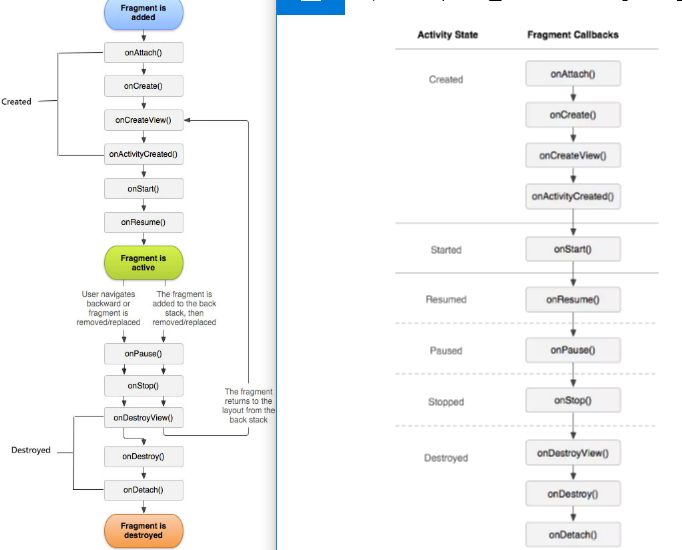
\includegraphics[width=.9\linewidth]{./pic/fragmentlifecycle2.png}
\item fragment所生存的activity生命周期直接影响着fragment的生命周期,由此针对activity的每一个生命周期回调都会引发一个fragment类似的回调。例如,当activity接收到onPause()时,这个activity之中的每个fragment都会接收到onPause()。
\end{itemize}
[这有Activity的详细说明](\url{http://blog.csdn.net/amazing7/article/details/51244219})
\begin{itemize}
\item Fragment有一些额外的生命周期回调方法(创建和销毁fragment界面).
\begin{itemize}
\item onAttach()
\begin{itemize}
\item 当fragment被绑定到activity时调用(Activity会被传入)。
\end{itemize}
\item onCreateView()
\begin{itemize}
\item 将本身的布局构建到activity中去(fragment作为activity界面的一部分)
\end{itemize}
\item onActivityCreated()
\begin{itemize}
\item 当activity的onCreate()函数返回时被调用。
\end{itemize}
\item onDestroyView()
\begin{itemize}
\item 当与fragment关联的视图体系正被移除时被调用。
\end{itemize}
\item onDetach()
\begin{itemize}
\item 当fragment正与activity解除关联时被调用。
\end{itemize}
\end{itemize}
\item 当activity接收到它的onCreate()回调时,activity之中的fragment接收到onActivityCreated()回调。
\begin{itemize}
\item 一旦activity处于resumed状态,则可以在activity中自由的添加或者移除fragment。因此,只**有当activity处于resumed状态时**,fragment的生命周期才可以独立变化。fragment会在 activity离开恢复状态时 再一次被activity推入它的生命周期中。
\end{itemize}
\item \textbf{管理fragment生命周期} 与管理activity生命周期很相像。像activity一样,fragment也有三种状态:
\begin{itemize}
\item Resumed
\begin{itemize}
\item fragment在运行中的activity可见。
\end{itemize}
\item Paused
\begin{itemize}
\item 另一个activity处于前台且得到焦点,但是这个fragment所在的activity仍然可见(前台activity部分透明,或者没有覆盖全屏)。
\end{itemize}
\item Stopped
\begin{itemize}
\item fragment不可见。要么宿主activity已经停止,要么fragment已经从activity上移除,但已被添加到后台栈中。一个停止的fragment仍然活着(所有状态和成员信息仍然由系统保留着)。但是,它对用户来讲已经不再可见,并且如果activity被杀掉,它也将被杀掉。
\item 如果activity的进程被杀掉了,在activity被重新创建时,你需要恢复fragment状态。可以执行fragment的onSaveInstanceState()来保存状态(注意在fragment是在onCreate(),onCreateView(),或onActvityCreate()中进行恢复)。
\end{itemize}
\end{itemize}
\item 在生命周期方面,activity与fragment之间一个 \textbf{很重要的不同} ,就是在各自的后台栈中是如何存储的。
\begin{itemize}
\item 当activity停止时,默认情况下activity被安置在由系统管理的activity后台栈中; 
\item fragment仅当在一个事务被移除时,通过显式调用addToBackStack()请求保存的实例,该fragment才被置于由宿主activity管理的后台栈。 
\end{itemize}
\item \textbf{要创建一个fragment} ,必须创建一个fragment的子类。一般情况下,我们至少需要实现以下几个fragment生命周期方法:
\begin{itemize}
\item onCreate()
\begin{itemize}
\item 在创建fragment时系统会调用此方法。在实现代码中,你可以初始化想要在fragment中保持的那些必要组件,当fragment处于暂停或者停止状态之后可重新启用它们。
\end{itemize}
\item onCreateView()
\begin{itemize}
\item 在第一次为fragment绘制用户界面时系统会调用此方法。为fragment绘制用户界面,这个函数必须要返回所绘出的fragment的根View。如果fragment没有用户界面可以返回空。
\end{itemize}
\end{itemize}
\begin{minted}[frame=lines,fontsize=\scriptsize,linenos=false]{java}
@Override
public View onCreateView(LayoutInflater inflater, ViewGroup container,
                         Bundle savedInstanceState) { 
    // Inflate the layout for this fragment
    return inflater.inflate(R.layout.example_fragment, container, false);
}
\end{minted}
\begin{itemize}
\item inflate()函数需要以下三个参数:
\begin{itemize}
\item ①要inflate的布局的资源ID。 
\item ②被inflate的布局的父ViewGroup。
\item ③一个布尔值,表明在inflate期间被infalte的布局是否应该附上ViewGroup(第二个参数container)。(在这个例子中传入的是false,因为系统已经将被inflate的布局插入到容器中(container)——传入true会在最终的布局里创建一个多余的ViewGroup。) 
\end{itemize}
\item onPause()
\begin{itemize}
\item 系统回调用该函数作为用户离开fragment的第一个预兆(尽管这并不总意味着fragment被销毁)。在当前用户会话结束之前,通常要在这里提交任何应该持久化的变化(因为用户可能不再返回)。
\end{itemize}
\end{itemize}
\end{itemize}

\subsection{将fragment添加到activity之中}
\label{sec-2-3}
\begin{itemize}
\item 可以通过在activity布局文件中声明fragment,用fragment标签把fragment插入到activity的布局中,或者是用应用程序源码将它添加到一个存在的ViewGroup中。 
\item 但fragment并不是一个定要作为activity布局的一部分,fragment也可以为activity隐身工作。
\end{itemize}
\subsubsection{在activity的布局文件里声明fragment}
\label{sec-2-3-1}
\begin{itemize}
\item 可以像为view一样为fragment指定布局属性。例如:
\begin{minted}[frame=lines,fontsize=\scriptsize,linenos=false]{xml}
<?xml version="1.0" encoding="utf-8"?>
<LinearLayout xmlns:android="http://schemas.android.com/apk/res/android"
      android:orientation="horizontal"
      android:layout_width="match_parent"
      android:layout_height="match_parent"> 
<fragment android:name="com.example.test.FragmentOne"
      android:id="@+id/fo"
      android:layout_width="match_parent"
      android:layout_height="match_parent" />
</LinearLayout>
\end{minted}
\item fragment标签中的android:name 属性指定了布局中实例化的Fragment类。
\item 当系统创建activity布局时,它实例化了布局文件中指定的每一个fragment,并为它们调用onCreateView()函数,以获取每一个fragment的布局。系统直接在<fragment>元素的位置插入fragment返回的View。
\item 注意:每个fragment都需要一个唯一的标识,如果重启activity,系统可用来恢复fragment(并且可用来捕捉fragment的事务处理,例如移除)。
\item 为fragment提供ID有三种方法:
\begin{itemize}
\item 用android:id属性提供一个唯一的标识。 
\item 用android:tag属性提供一个唯一的字符串。 
\item 如果上述两个属性都没有,系统会使用其容器视图(view)的ID。 
\end{itemize}
\end{itemize}
\subsubsection{通过编码将fragment添加到已存在的ViewGroup中}
\label{sec-2-3-2}
\begin{itemize}
\item 在activity运行的任何时候,你都可以将fragment添加到activity布局中。
\item 要管理activity中的fragment,可以使用FragmentManager。可以通过在activity中调用getFragmentManager()获得。使用FragmentManager 可以做如下事情,包括:
\begin{itemize}
\item 使用findFragmentById()(用于在activity布局中提供有界面的fragment)或者findFragmentByTag()获取activity中存在的fragment(用于有界面或者没有界面的fragment)。  
\item 使用popBackStack()(模仿用户的BACK命令)从后台栈弹出fragment。  
\item 使用addOnBackStackChangedListener()注册一个监听后台栈变化的监听器。
\end{itemize}
\item 在Android中,对Fragment的事务操作都是通过FragmentTransaction来执行。操作大致可以分为两类:
\begin{itemize}
\item 显示:add() replace() show() attach()  
\item 隐藏:remove() hide() detach() 
\item 说明:
\begin{itemize}
\item 调用show() \& hide()方法时,Fragment的生命周期方法并不会被执行,仅仅是Fragment的View被显示或者​隐藏。
\item 执行replace()时(至少两个Fragment),会执行第二个Fragment的onAttach()方法、执行第一个Fragment的onPause()-onDetach()方法,同时containerView会detach第一个Fragment的View。
\item add()方法执行onAttach()-onResume()的生命周期,相对的remove()就是执行完成剩下的onPause()-onDetach()周期。
\end{itemize}
\end{itemize}
\item 可以像下面这样从Activity中取得FragmentTransaction的实例:
\begin{minted}[frame=lines,fontsize=\scriptsize,linenos=false]{java}
FragmentManager fragmentManager = getFragmentManager() 
FragmentTransaction fragmentTransaction = fragmentManager.beginTransaction();
\end{minted}
\item 可以用add()函数添加fragment,并指定要添加的fragment以及要将其插入到哪个视图(view)之中(注意commit事务):
\begin{minted}[frame=lines,fontsize=\scriptsize,linenos=false]{java}
ExampleFragment fragment = new ExampleFragment();
fragmentTransaction.add(R.id.fragment_container, fragment);
fragmentTransaction.commit();
\end{minted}
\end{itemize}
\subsubsection{添加没有界面的fragment}
\label{sec-2-3-3}
\begin{itemize}
\item 也可以使用fragment为activity提供后台动作,却不呈现多余的用户界面。
\item 想要添加没有界面的fragment ,可以使用add(Fragment, String)(为fragment提供一个唯一的字符串“tag”,而不是视图(view)ID)。这样添加了fragment,但是,因为还没有关联到activity布局中的视图(view) ,收不到onCreateView()的调用。所以不需要实现这个方法。 
\item 对于无界面fragment,字符串标签是**唯一识别**它的方法。如果之后想从activity中取到fragment,需要使用findFragmentByTag()。 
\end{itemize}
\subsection{fragment事务后台栈}
\label{sec-2-4}
\begin{itemize}
\item 在调用commit()之前,可以将事务添加到fragment事务后台栈中(通过调用addToBackStack())。这个后台栈由activity管理,并且允许用户通过按BACK键回退到前一个fragment状态。
\item 下面的代码中一个fragment代替另一个fragment,并且将之前的fragment状态保留在后台栈中:
\begin{minted}[frame=lines,fontsize=\scriptsize,linenos=false]{java}
 Fragment newFragment = new ExampleFragment();
 FragmentTransaction transaction = getFragmentManager().beginTransaction();
 transaction.replace(R.id.fragment_container, newFragment);
 transaction.addToBackStack(null);
 transaction.commit();
\end{minted}
\item 注意:
\begin{itemize}
\item 如果添加多个变更事务(例如另一个add()或者remove())并调用addToBackStack(),那么在调用commit()之前的所有应用的变更被作为一个单独的事务添加到后台栈中,并且BACK键可以将它们一起回退。
\item 当移除一个fragment时,如果调用了addToBackStack(),那么之后fragment会被停止,如果用户回退,它将被恢复过来。
\item 调用commit()并不立刻执行事务,相反,而是采取预约方式,一旦activity的界面线程(主线程)准备好便可运行起来。然而,如果有必要的话,你可以从界面线程调用executePendingTransations()立即执行由commit()提交的事务。
\item 只能在activity保存状态(当用户离开activity时)之前用commit()提交事务。如果你尝试在那时之后提交,会抛出一个异常。这是因为如果activity需要被恢复,提交后的状态会被丢失。对于这类丢失提交的情况,可使用commitAllowingStateLoss()
\end{itemize}
\end{itemize}
\subsection{与Activity交互}
\label{sec-2-5}
\begin{itemize}
\item Activity中已经有了该Fragment的引用,直接通过该引用进行交互。
\begin{itemize}
\item 如果没引用可以通过调用fragment的函数findFragmentById()或者findFragmentByTag(),从FragmentManager中获取Fragment的索引,例如:
\end{itemize}
\begin{minted}[frame=lines,fontsize=\scriptsize,linenos=false]{java}
ExampleFragment fragment = (ExampleFragment) getFragmentManager().findFragmentById(R.id.example_fragment);
\end{minted}
\begin{itemize}
\item 在Fragment中可以通过getActivity得到当前绑定的Activity的实例。
\item 创建activity事件回调函数,在fragment内部定义一个回调接口,宿主activity来实现它。
\end{itemize}
\end{itemize}

\section{Service全面总结}
\label{sec-3}
\subsection{什么是服务?  }
\label{sec-3-1}
\begin{itemize}
\item Service是一个应用程序组件,它能够在后台执行一些耗时较长的操作,并且不提供用户界面。服务能被其它应用程序的组件启动,即使用户切换到另外的应用时还能保持后台运行。此外,应用程序组件还能与服务绑定,并与服务进行交互,甚至能进行进程间通信(IPC)。 比如,服务可以处理网络传输、音乐播放、执行文件I/O、或者与content provider进行交互,所有这些都是后台进行的。
\end{itemize}
\subsection{Service 与 Thread 的区别}
\label{sec-3-2}
\begin{itemize}
\item 服务仅仅是一个组件,即使用户不再与你的应用程序发生交互,它仍然能在后台运行。因此,应该只在需要时才创建一个服务。
\item 如果你需要在主线程之外执行一些工作,但仅当用户与你的应用程序交互时才会用到,那你应该创建一个新的线程而不是创建服务。 比如,如果你需要播放一些音乐,但只是当你的activity在运行时才需要播放,你可以在onCreate()中创建一个线程,在onStart()中开始运行,然后在onStop()中终止运行。还可以考虑使用AsyncTask或HandlerThread来取代传统的Thread类。
\item \textbf{由于无法在不同的 Activity 中对同一 Thread 进行控制} ,这个时候就要考虑用服务实现。如果你使用了服务,它默认就运行于应用程序的主线程中。因此,如果服务执行密集计算或者阻塞操作,你仍然应该在服务中创建一个新的线程来完成(避免ANR)。
\end{itemize}
\subsection{服务的分类}
\label{sec-3-3}
\subsubsection{按运行分类}
\label{sec-3-3-1}
\begin{itemize}
\item 前台服务
\begin{itemize}
\item 前台服务是指那些经常会被用户关注的服务,因此内存过低时它不会成为被杀的对象。 前台服务必须提供一个状态栏通知,并会置于“正在进行的”(“Ongoing”)组之下。这意味着只有在服务被终止或从前台移除之后,此通知才能被解除。
\item 例如,用服务来播放音乐的播放器就应该运行在前台,因为用户会清楚地知晓它的运行情况。 状态栏通知可能会标明当前播放的歌曲,并允许用户启动一个activity来与播放器进行交互。
\item 要把你的服务请求为前台运行,可以调用startForeground()方法。此方法有两个参数:唯一标识通知的整数值、状态栏通知Notification对象。例如:
\end{itemize}
\begin{minted}[frame=lines,fontsize=\scriptsize,linenos=false]{java}
Notification notification = new Notification(R.drawable.icon,
                                             getText(R.string.ticker_text),
                                             System.currentTimeMillis());
Intent notificationIntent = new Intent(this,ExampleActivity.class);
PendingIntent pendingIntent = PendingIntent.getActivity(this, 0,
                                                        notificationIntent, 0);
notification.setLatestEventInfo(this, getText(R.string.notification_title),
                                getText(R.string.notification_message),
                                pendingIntent);
startForeground(ONGOING_NOTIFICATION, notification);
\end{minted}
\begin{itemize}
\item 要从前台移除服务,请调用stopForeground()方法,这个方法接受个布尔参数,表示是否同时移除状态栏通知。此方法不会终止服务。不过,如果服务在前台运行时被你终止了,那么通知也会同时被移除。
\end{itemize}
\item 后台服务
\end{itemize}
\subsubsection{按使用分类  }
\label{sec-3-3-2}
\begin{itemize}
\item 本地服务
\begin{itemize}
\item 用于应用程序内部,实现一些耗时任务,并不占用应用程序比如Activity所属线程,而是单开线程后台执行。
\item 调用Context.startService()启动,调用Context.stopService()结束。在内部可以调用Service.stopSelf() 或 Service.stopSelfResult()来自己停止。
\end{itemize}
\item 远程服务
\begin{itemize}
\item 用于Android系统内部的应用程序之间,可被其他应用程序复用,比如天气预报服务,其他应用程序不需要再写这样的服务,调用已有的即可。可以定义接口并把接口暴露出来,以便其他应用进行操作。客户端建立到服务对象的连接,并通过那个连接来调用服务。调用Context.bindService()方法建立连接,并启动,以调用 Context.unbindService()关闭连接。多个客户端可以绑定至同一个服务。如果服务此时还没有加载,bindService()会先加载它。
\end{itemize}
\end{itemize}
\subsection{Service生命周期}
\label{sec-3-4}

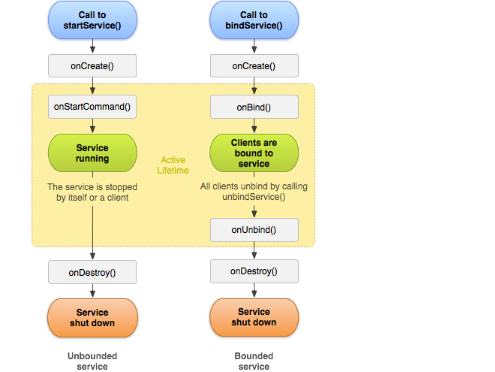
\includegraphics[width=.9\linewidth]{./pic/servicelifecycle.png}
\begin{itemize}
\item Service生命周期方法:
\begin{minted}[frame=lines,fontsize=\scriptsize,linenos=false]{java}
public class ExampleService extends Service {
    int mStartMode;       // 标识服务被杀死后的处理方式
    IBinder mBinder;      // 用于客户端绑定的接口
    boolean mAllowRebind; // 标识是否使用onRebind
    @Override
    public void onCreate() {
        // 服务正被创建
    }
    @Override
    public int onStartCommand(Intent intent, int flags, int startId) {
        // 服务正在启动,由startService()调用引发
        return mStartMode;
    }
    @Override
    public IBinder onBind(Intent intent) {
        // 客户端用bindService()绑定服务
        return mBinder;
    }
    @Override
    public boolean onUnbind(Intent intent) {
        // 所有的客户端都用unbindService()解除了绑定
        return mAllowRebind;
    }
    @Override
    public void onRebind(Intent intent) {
        // 某客户端正用bindService()绑定到服务,
        // 而onUnbind()已经被调用过了
    }
    @Override
    public void onDestroy() {
        // 服务用不上了,将被销毁
    }
}
\end{minted}
\begin{itemize}
\item 请注意onStartCommand()方法必须返回一个整数。这个整数是描述系统在杀死服务之后应该如何继续运行。onStartCommand()的返回值必须是以下常量之一:
\begin{itemize}
\item START\_NOT\_STICKY  
\begin{itemize}
\item 如果系统在onStartCommand()返回后杀死了服务,则不会重建服务了,除非还存在未发送的intent。 当服务不再是必需的,并且应用程序能够简单地重启那些未完成的工作时,这是避免服务运行的最安全的选项。 
\end{itemize}
\item START\_STICKY 
\begin{itemize}
\item 如果系统在onStartCommand()返回后杀死了服务,则将重建服务并调用onStartCommand(),但不会再次送入上一个intent, 而是用null intent来调用onStartCommand() 。除非还有启动服务的intent未发送完,那么这些剩下的intent会继续发送。 这适用于媒体播放器(或类似服务),它们不执行命令,但需要一直运行并随时待命。 
\end{itemize}
\item START\_REDELIVER\_INTENT 
\begin{itemize}
\item 如果系统在onStartCommand()返回后杀死了服务,则将重建服务并用上一个已送过的intent调用onStartCommand()。任何未发送完的intent也都会依次送入。这适用于那些需要立即恢复工作的活跃服务,比如下载文件。
\end{itemize}
\end{itemize}
\end{itemize}
\item 服务的生命周期与activity的非常类似。不过,更重要的是你需密切关注服务的创建和销毁环节,因为后台运行的服务是不会引起用户注意的。
\item 服务的生命周期——从创建到销毁——可以有两种路径:
\begin{itemize}
\item 一个started服务
\begin{itemize}
\item 这类服务由其它组件调用startService()来创建。然后保持运行,且必须通过调用stopSelf()自行终止。其它组件也可通过调用stopService() 终止这类服务。服务终止后,系统会把它销毁。
\item 如果一个Service被startService 方法多次启动,那么onCreate方法只会调用一次,onStart将会被调用多次(对应调用startService的次数),并且系统只会创建Service的一个实例(因此你应该知道只需要一次stopService调用)。该Service将会一直在后台运行,而不管对应程序的Activity是否在运行,直到被调用stopService,或自身的stopSelf方法。当然如果系统资源不足,android系统也可能结束服务。
\end{itemize}
\item 一个bound服务
\begin{itemize}
\item 服务由其它组件(客户端)调用bindService()来创建。然后客户端通过一个IBinder接口与服务进行通信。客户端可以通过调用unbindService()来关闭联接。多个客户端可以绑定到同一个服务上,当所有的客户端都解除绑定后,系统会销毁服务。(服务不需要自行终止。)
\item 如果一个Service被某个Activity 调用 Context.bindService 方法绑定启动,不管调用 bindService 调用几次,onCreate方法都只会调用一次,同时onStart方法始终不会被调用。当连接建立之后,Service将会一直运行,除非调用Context.unbindService 断开连接或者之前调用bindService 的 Context 不存在了(如Activity被finish的时候),系统将会自动停止Service,对应onDestroy将被调用。
\end{itemize}
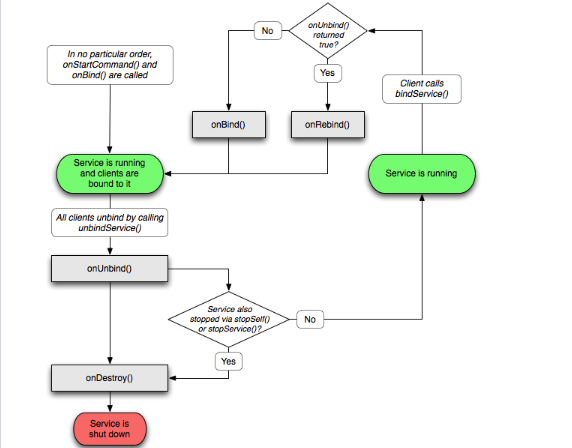
\includegraphics[width=.9\linewidth]{./pic/service2.png}
\end{itemize}
\item 这两条路径并不是完全隔离的。也就是说,你可以绑定到一个已经用startService()启动的服务上。例如,一个后台音乐服务可以通过调用startService()来启动,传入一个指明所需播放音乐的 Intent。 之后,用户也许需要用播放器进行一些控制,或者需要查看当前歌曲的信息,这时一个activity可以通过调用bindService()与此服务绑定。在类似这种情况下,stopService()或stopSelf()不会真的终止服务,除非所有的客户端都解除了绑定。
\begin{itemize}
\item 当在旋转手机屏幕的时候,当手机屏幕在“横”“竖”变换时,此时如果你的 Activity 如果会自动旋转的话,旋转其实是 Activity 的重新创建,因此旋转之前的使用 bindService 建立的连接便会断开(Context 不存在了)。
\end{itemize}
\end{itemize}
\subsection{在manifest中声明服务}
\label{sec-3-5}
\begin{itemize}
\item 无论是什么类型的服务都必须在manifest中申明,格式如下:
\begin{minted}[frame=lines,fontsize=\scriptsize,linenos=false]{xml}
<manifest ... >
  <application ... >
      <service android:name=".ExampleService" />
  </application>
</manifest>
\end{minted}
\item Service 元素的属性有:
\end{itemize}
\begin{center}
\begin{tabular}{ll}
\hline
android:name & 服务类名\\
android:label & 服务的名字.如果此项不设置,那么默认显示的服务名则为类名\\
android:icon & 服务的图标\\
android:permission & 申明此服务的权限,这意味着只有提供了该权限的应用才能控制或连接此服务\\
android:process & 表示该服务是否运行在另外一个进程,\\
 & 如果设置了此项,那么将会在包名后面加上这段字符串表示另一进程的名字\\
android:enabled & 如果此项设置为 true,那么 Service 将会默认被系统启动,不设置默认此项为 false\\
android:exported & 表示该服务是否能够被其他应用程序所控制或连接,不设置默认此项为 false \\
\hline
\end{tabular}
\end{center}
\begin{itemize}
\item android:name是唯一必需的属性——它定义了服务的类名。与activity一样,服务可以定义intent过滤器,使得其它组件能用隐式intent来调用服务。如果你想让服务只能内部使用(其它应用程序无法调用),那么就不必(也不应该)提供任何intent过滤器。
\item 此外,如果包含了android:exported属性并且设置为"false", 就可以确保该服务是你应用程序的私有服务。即使服务提供了intent过滤器,本属性依然生效。 
\end{itemize}
\subsection{startService 启动服务}
\label{sec-3-6}
\begin{itemize}
\item 从activity或其它应用程序组件中可以启动一个服务,调用startService()并传入一个Intent(指定所需启动的服务)即可。
\begin{minted}[frame=lines,fontsize=\scriptsize,linenos=false]{java}
  Intent intent = new Intent(this, MyService.class);
  startService(intent);
\end{minted}
\item 服务类:
\begin{minted}[frame=lines,fontsize=\scriptsize,linenos=false]{java}
public class MyService extends Service {
     // onBind 是 Service 的虚方法,因此我们不得不实现它。
     // 返回 null,表示客服端不能建立到此服务的连接。
    @Override
    public IBinder onBind(Intent intent) {
        // TODO Auto-generated method stub
        return null;
    }
    @Override
    public void onCreate() {
        super.onCreate();
    }
    @Override
    public int onStartCommand(Intent intent, int flags, int startId) {
        //接受传递过来的intent的数据 
        return START_STICKY; 
    };
    @Override
    public void onDestroy() {
        super.onDestroy();
    }
}
\end{minted}
\item 一个started服务必须自行管理生命周期。也就是说,系统不会终止或销毁这类服务,除非必须恢复系统内存并且服务返回后一直维持运行。 因此,服务必须通过调用stopSelf()自行终止,或者其它组件可通过调用stopService()来终止它。
\end{itemize}
\subsection{bindService 启动服务  }
\label{sec-3-7}
\begin{itemize}
\item 当应用程序中的activity或其它组件需要与服务进行交互,或者应用程序的某些功能需要暴露给其它应用程序时,你应该创建一个bound服务,并通过进程间通信(IPC)来完成。
\item 方法如下:
\begin{minted}[frame=lines,fontsize=\scriptsize,linenos=false]{java}
 Intent intent=new Intent(this,BindService.class); 
 bindService(intent, ServiceConnection conn, int flags)
\end{minted}
\item 注意bindService是Context中的方法,当没有Context时传入即可。
\item 在进行服务绑定的时,其flags有:
\begin{itemize}
\item Context.BIND\_AUTO\_CREATE    
\begin{itemize}
\item 表示收到绑定请求的时候,如果服务尚未创建,则即刻创建,在系统内存不足需要先摧毁优先级组件来释放内存,且只有驻留该服务的进程成为被摧毁对象时,服务才被摧毁 
\end{itemize}
\item Context.BIND\_DEBUG\_UNBIND     
\begin{itemize}
\item 通常用于调试场景中判断绑定的服务是否正确,但容易引起内存泄漏,因此非调试目的的时候不建议使用
\end{itemize}
\item Context.BIND\_NOT\_FOREGROUND     
\begin{itemize}
\item 表示系统将阻止驻留该服务的进程具有前台优先级,仅在后台运行。
\end{itemize}
\end{itemize}
\item 服务类:
\begin{minted}[frame=lines,fontsize=\scriptsize,linenos=false]{java}
public class BindService extends Service {
    // 实例化MyBinder得到mybinder对象;
    private final MyBinder binder = new MyBinder();
    // 返回Binder对象。
    @Override
    public IBinder onBind(Intent intent) {
        // TODO Auto-generated method stub
        return binder;
    }
     // 新建内部类MyBinder,继承自Binder(Binder实现IBinder接口),
     // MyBinder提供方法返回BindService实例。
    public class MyBinder extends Binder{
        public BindService getService(){
            return BindService.this;
        }
    }
    @Override
    public boolean onUnbind(Intent intent) {
        // TODO Auto-generated method stub
        return super.onUnbind(intent);
    }
}
\end{minted}
\item 启动服务的activity代码:
\begin{minted}[frame=lines,fontsize=\scriptsize,linenos=false]{java}
public class MainActivity extends Activity {
    // 是否绑定 
    boolean mIsBound = false; 
    BindService mBoundService;
    @Override
    protected void onCreate(Bundle savedInstanceState) {
        super.onCreate(savedInstanceState);
        setContentView(R.layout.activity_main);
        doBindService();
    }
    // 实例化ServiceConnection接口的实现类,用于监听服务的状态
    private ServiceConnection conn = new ServiceConnection() {  
            @Override  
            public void onServiceConnected(ComponentName name, IBinder service) {  
                BindService mBoundService = ((BindService.MyBinder) service).getService();  
            
            }  
            @Override  
            public void onServiceDisconnected(ComponentName name) {  
                mBoundService = null;  
            }  
        }; 
    // 绑定服务 
    public void doBindService() {  
        bindService(new Intent(MainActivity.this, BindService.class), conn,Context.BIND_AUTO_CREATE);  
        mIsBound = true;  
    }  
    // 解除绑定服务
    public void doUnbindService() {  
        if (mIsBound) {  
            // Detach our existing connection.  
            unbindService(conn);  
            mIsBound = false;  
        }  
    } 
    @Override
    protected void onDestroy() {
        // TODO Auto-generated method stub
        super.onDestroy();
        doUnbindService();
    }
}
\end{minted}
\item 注意在AndroidMainfest.xml中对Service进行显式声明
\item 判断Service是否正在运行:
\begin{minted}[frame=lines,fontsize=\scriptsize,linenos=false]{java}
private boolean isServiceRunning() {
    ActivityManager manager = (ActivityManager) getSystemService(ACTIVITY_SERVICE);
    {
        if ("com.example.demo.BindService".equals(service.service.getClassName())) {
            return true;
        }
    }
    return false;
}
\end{minted}
\end{itemize}
\section{IntentService使用详解和实例但介绍}
\label{sec-4}
\subsection{IntentService定义}
\label{sec-4-1}
\begin{itemize}
\item IntentService继承与Service,用来处理异步请求。客户端可以通过startService(Intent)方法传递请求给IntentService。IntentService在onCreate()函数中通过HandlerThread单独开启一个线程来依次处理所有Intent请求对象所对应的任务。 
\item 这样以免事务处理阻塞主线程(ANR)。执行完所一个Intent请求对象所对应的工作之后,如果没有新的Intent请求达到,则**自动停止**Service;否则执行下一个Intent请求所对应的任务。 
\item IntentService在处理事务时,还是采用的Handler方式,创建一个名叫ServiceHandler的内部Handler,并把它直接绑定到HandlerThread所对应的子线程。 ServiceHandler把处理一个intent所对应的事务都封装到叫做**onHandleIntent**的虚函数;因此我们直接实现虚函数onHandleIntent,再在里面根据Intent的不同进行不同的事务处理就可以了。
\item 另外,IntentService默认实现了Onbind()方法,返回值为null。
\item 使用IntentService需要实现的两个方法:
\begin{itemize}
\item 构造函数 
\begin{itemize}
\item IntentService的构造函数一定是**参数为空**的构造函数,然后再在其中调用super("name")这种形式的构造函数。因为Service的实例化是系统来完成的,而且系统是用参数为空的构造函数来实例化Service的
\end{itemize}
\item 实现虚函数onHandleIntent
\begin{itemize}
\item 在里面根据Intent的不同进行不同的事务处理。 
\item 好处:处理异步请求的时候可以减少写代码的工作量,比较轻松地实现项目的需求。
\end{itemize}
\end{itemize}
\end{itemize}
\subsection{IntentService与Service的区别}
\label{sec-4-2}
\begin{itemize}
\item Service不是独立的进程,也不是独立的线程,它是依赖于应用程序的主线程的,不建议在Service中编写耗时的逻辑和操作,否则会引起ANR。
\item IntentService 它创建了一个独立的工作线程来处理所有的通过onStartCommand()传递给服务的intents(把intent插入到工作队列中)。通过工作队列把intent逐个发送给onHandleIntent()。 
\item 不需要主动调用stopSelft()来结束服务。因为,在所有的intent被处理完后,系统会自动关闭服务。
\item 默认实现的onBind()返回null。
\end{itemize}
\subsection{IntentService实例介绍}
\label{sec-4-3}
\begin{itemize}
\item 首先是myIntentService.java
\begin{minted}[frame=lines,fontsize=\scriptsize,linenos=false]{java}
public class myIntentService extends IntentService {
    //------------------必须实现-----------------------------
    public myIntentService() {
        super("myIntentService");
        // 注意构造函数参数为空,这个字符串就是worker thread的名字
    }
    @Override
    protected void onHandleIntent(Intent intent) {
        //根据Intent的不同进行不同的事务处理 
        String taskName = intent.getExtras().getString("taskName");  
        switch (taskName) {
        case "task1":
            Log.i("myIntentService", "do task1");
            break;
        case "task2":
            Log.i("myIntentService", "do task2");
            break;
        default:
            break;
        }        
    }
    //--------------------用于打印生命周期--------------------    
    @Override
    public void onCreate() {
        Log.i("myIntentService", "onCreate");
        super.onCreate();
    }
    @Override
    public int onStartCommand(Intent intent, int flags, int startId) {
        Log.i("myIntentService", "onStartCommand");
        return super.onStartCommand(intent, flags, startId);
    }
    @Override
    public void onDestroy() {
        Log.i("myIntentService", "onDestroy");
        super.onDestroy();
    }
}
\end{minted}
\item 然后记得在Manifest.xml中注册服务
\begin{minted}[frame=lines,fontsize=\scriptsize,linenos=false]{xml}
<service android:name=".myIntentService">
  <intent-filter >  
    <action android:name="cn.scu.finch"/>  
  </intent-filter>     
</service>
\end{minted}
\item 最后在Activity中开启服务
\begin{minted}[frame=lines,fontsize=\scriptsize,linenos=false]{java}
public class MainActivity extends Activity {
    @Override
    protected void onCreate(Bundle savedInstanceState) {
        // TODO Auto-generated method stub
        super.onCreate(savedInstanceState);
        //同一服务只会开启一个worker thread,在onHandleIntent函数里依次处理intent请求。
        Intent i = new Intent("cn.scu.finch");  
        Bundle bundle = new Bundle();  
        bundle.putString("taskName", "task1");  
        i.putExtras(bundle);  
        startService(i);  
        Intent i2 = new Intent("cn.scu.finch");  
        Bundle bundle2 = new Bundle();  
        bundle2.putString("taskName", "task2");  
        i2.putExtras(bundle2);  
        startService(i2); 
        startService(i);  //多次启动
    }
}
\end{minted}
\item 运行结果:
\begin{minted}[frame=lines,fontsize=\scriptsize,linenos=false]{text}
myIntentService onCreate()
myIntentService onStartCommand()
myIntentService onStartCommand()
myIntentService do task1
myIntentService onStartCommand()
myIntentService do task2
myIntentService do task1
myIntentService onDestroy()
\end{minted}
\item IntentService在onCreate()函数中通过HandlerThread单独开启一个线程来依次处理所有Intent请求对象所对应的任务。 
\item 通过onStartCommand()传递给服务intent被**依次**插入到工作队列中。工作队列又把intent逐个发送给onHandleIntent()。
\item 注意:
\begin{itemize}
\item 它只有一个工作线程,名字就是构造函数的那个字符串,也就是“myIntentService”,我们知道多次开启service,只会调用一次onCreate方法(创建一个工作线程),多次onStartCommand方法(用于传入intent通过工作队列再发给onHandleIntent函数做处理)。
\end{itemize}
\end{itemize}

\section{Android启动过程图解}
\label{sec-5}
Android手机开机执行过程图:
![这里写图片描述](\url{http://img.blog.csdn.net/20160603133621981}) 
从开机到桌面的过程为:
\textbf{\textbf{Bootloader}} ➪**Kernel** ➪**Init进程** ➪ \textbf{\textbf{Zygote}} ➪ \textbf{\textbf{SystemServer}} ➪ \textbf{\textbf{ServiceManager}} ➪ \textbf{\textbf{Home Launcher}}
Android服务包括系统服务和应用服务,系统服务是指Android系统在启动过程就已经启动实现了的服务,对于系统服务又分为Java服务和本地服务,Java服务是由Java代码编写而成,由SystemServer进程提供,而本地服务是由C/C++实现的服务,由Init进程在系统启动时启动的服务。应用服务是由开发者自行实现的某些特定服务。
 1、Bootloader
\subsubsection{}
\label{sec-5-0-1}
当电源按下,引导芯片代码开始从预定义的地方(固化在ROM)开始执行。加载引导程序到RAM,然后执行。
BootLoader是在操作系统内核运行之前运行。可以初始化硬件设备、建立内存空间映射图,从而将系统的软硬件环境带到一个合适状态,以便为最终调用操作系统内核准备好正确的环境。
 2、Kernel
\subsubsection{}
\label{sec-5-0-2}
Android内核启动时,会设置缓存、被保护存储器、计划列表,加载驱动。当内核完成系统设置,它首先在系统文件中寻找”init”文件,然后启动root进程或者系统的第一个进程。
 3、init进程
\subsubsection{}
\label{sec-5-0-3}
init进程,它是一个由内核启动的用户级进程。内核自行启动(已经被载入内存,开始运行,并已初始化所有的设备驱动程序和数据结构等)之后,就通过启动一个用户级程序init的方式,完成引导进程。init始终是第一个进程。
启动过程就是代码init.c中main函数执行过程:system\core\init\init.c在函数中执行了:**文件夹建立**,**挂载**,**rc文件解析**,**属性设置**,**启动服务**,**执行动作**,**socket监听**……
\begin{itemize}
\item rc文件解析
\end{itemize}
.rc文件是Android使用的初始化脚本文件 ,Android中有特定的格式以及规则。
 4、Zygote
\subsubsection{}
\label{sec-5-0-4}
所有的应用程序进程以及系统服务进程(SystemServer)都是由Zygote进程孕育(fork)出来的,zygote本身是Native应用程序,与驱动内核无关。
我们知道,Android系统是基于Linux内核的,而在Linux系统中,所有的进程都是init进程的子孙进程,也就是说,所有的进程都是直接或者间接地由init进程fork出来的。Zygote进程也不例外,它是在系统启动的过程,由init进程创建的(在系统启动脚本system/core/rootdir/init.rc文件中)。
在Java中,不同的虚拟机实例会为不同的应用分配不同的内存。假如Android应用应该尽可能快地启动,但如果Android系统为每一个应用启动不同的Dalvik虚拟机实例,就会消耗大量的内存以及时间。因此,为了克服这个问题,Android系统创造了”Zygote”。Zygote是一个虚拟器进程,预加载以及初始化核心库类,让Dalvik虚拟机共享代码、降低内存占用和启动时间。
\textbf{\textbf{Zygote进程包含两个主要模块:}}
  ①. Socket服务端,该Socket服务端用于接收启动新的Dalvik进程命令。
  ②. Framework共享类及共享资源,当Zygote进程启动后,会装载一些共享类和资源,共享类是在preload-classes文件中定义的,共享资源是在preload-resources文件中定义。因为其他Dalvik进程是由Zygote进程孵化出来的,因此只要Zygote装载好了这些类和资源后,新的Dalvik进程就不需要在装载这些类和资源了,它们共享Zygote进程的资源和类。
\textbf{\textbf{Zygote启动分为两个阶段:}}
  ①. **虚拟机启动 --- 通过native启动** 
\begin{itemize}
\item startVm(\&mJavaVM, \&env)   启动虚拟机 
\item onVmCreated(env)         虚拟机启动后的初始化
\item startReg(env)             注册JNI函数
\item env->CallStaticVoidMethod(startClass, startMeth, strArray) 调用ZygoteInit类的main函数开创java世界 
\end{itemize}
          
 ②. **SystemServer进程 --- 通过Java启动** 
\begin{itemize}
\item registerZygoteSocket()  为zygote进程注册监听socket
\item preload()            加载常用的JAVA类和系统资源
\item startSystemServer()    启动SystemServer进程
\item runSelectLoopMode()  进入循环监听模式
\item closeServerSocket()    进程退出时,关闭socket监听
5、启动系统服务
\end{itemize}
\subsubsection{}
\label{sec-5-0-5}
Zygote创建新的进程去启动系统服务。你可以在ZygoteInit类的”startSystemServer”方法中找到源代码。
核心服务:
\begin{itemize}
\item 启动电源管理器; 
\item 
\end{itemize}
创建Activity管理器; 
启动电话注册; 
启动包管理器;
设置Activity管理服务为系统进程;
启动上下文管理器;
启动系统Context Providers;
启动电池服务;
启动定时管理器;
启动传感服务;
启动窗口管理器;
启动蓝牙服务;
启动挂载服务。
其他服务:
 6、引导完成
\subsubsection{}
\label{sec-5-0-6}
一旦系统服务在内存中跑起来了,Android就完成了引导过程。在这个时候“ACTION\_BOOT\_COMPLETED”开机启动广播就会发出去。
\section{Android 异步消息处理机制(Handler 、 Looper 、MessageQueue)源码解析}
\label{sec-6}
1、Handler的由来
\subsubsection{}
\label{sec-6-0-1}
   当程序第一次启动的时候,Android会同时启动一条主线程( Main Thread)来负责处理与UI相关的事件,我们叫做UI线程。
Android的UI操作并不是线程安全的(出于性能优化考虑),意味着如果多个线程并发操作UI线程,可能导致线程安全问题。 
为了解决Android应用多线程问题—Android平台只允许UI线程修改Activity里的UI组建,就会导致新启动的线程无法改变界面组建的属性值。
**简单的说:**当主线程队列处理一个消息超过5秒,android 就会抛出一个 ANP(无响应)的异常,所以,我们需要把一些要处理比较长的消息,放在一个单独线程里面处理,把处理以后的结果,返回给主线程运行,就需要用的Handler来进行线程建的通信。
 2、Handler的作用
\subsubsection{}
\label{sec-6-0-2}
2.1 让线程延时执行
主要用到的两个方法:
\begin{itemize}
\item final boolean    postAtTime(Runnable r, long uptimeMillis)
\item final boolean    postDelayed(Runnable r, long delayMillis)
\end{itemize}
2.2 让任务在其他线程中执行并返回结果
分为两个步骤:
\begin{itemize}
\item 在新启动的线程中发送消息
\end{itemize}
使用Handler对象的sendMessage()方法或者SendEmptyMessage()方法发送消息。
\begin{itemize}
\item 在主线程中获取处理消息
\end{itemize}
重写Handler类中处理消息的方法(void handleMessage(Message msg)),当新启动的线程发送消息时,消息发送到与之关联的MessageQueue。而Hanlder不断地从MessageQueue中获取并处理消息。
 3、Handler更新UI线程一般使用
\subsubsection{}
\label{sec-6-0-3}
\begin{itemize}
\item 首先要进行Handler 申明,复写handleMessage方法( 放在主线程中)
\end{itemize}
private Handler handler = new Handler() \{
        @Override
        public void handleMessage(Message msg) \{
            // TODO 接收消息并且去更新UI线程上的控件内容
            if (msg.what == UPDATE) \{
                // 更新界面上的textview
                tv.setText(String.valueOf(msg.obj));
            \}
            super.handleMessage(msg);
        \}
    \};
\begin{itemize}
\item 子线程发送Message给ui线程表示自己任务已经执行完成,主线程可以做相应的操作了。
\end{itemize}
new Thread() \{
            @Override
            public void run() \{
                // TODO 子线程中通过handler发送消息给handler接收,由handler去更新TextView的值
                try \{
                       //do something

                       Message msg = new Message();
                       msg.what = UPDATE;                    
                       msg.obj = "更新后的值" ;
                       handler.sendMessage(msg);
                   \}
               \} catch (InterruptedException e) \{
                   e.printStackTrace();
               \}
           \}
       \}.start();
4、Handler原理分析
\subsubsection{}
\label{sec-6-0-4}
4.1  Handler的构造函数
\begin{itemize}
\item ① public Handler()
\end{itemize}
② public Handler(Callbackcallback)
③ public Handler(Looperlooper)
④ public Handler(Looperlooper, Callbackcallback)  
\begin{itemize}
\item 第①个和第②个构造函数都没有传递Looper,这两个构造函数都将通过调用Looper.myLooper()获取当前线程绑定的Looper对象,然后将该Looper对象保存到名为mLooper的成员字段中。  
\end{itemize}
下面来看①②个函数源码:
113    public Handler() \{
114        this(null, false);
115    \}
127    public Handler(Callback callback) \{
128        this(callback, false);
129    \}
//他们会调用Handler的内部构造方法
188    public Handler(Callback callback, boolean async) \{
189        if (FIND\_POTENTIAL\_LEAKS) \{
190      final Class<? extends Handler> klass = getClass();
191      if ((klass.isAnonymousClass() ||klass.isMemberClass()
\begin{center}
\begin{tabular}{ll}
 & klass.isLocalClass()) \&\&\\
\end{tabular}
\end{center}
192                    (klass.getModifiers() \& Modifier.STATIC) == 0) \{
193                Log.w(TAG, "The following Handler class should be static or leaks might occur: " +
194                    klass.getCanonicalName());
195            \}
196        \}
197/************************************
198        mLooper = Looper.myLooper();
199        if (mLooper == null) \{
200            throw new RuntimeException(
201                "Can't create handler inside thread that has not called Looper.prepare()");
202        \}
203        mQueue = mLooper.mQueue;
204        mCallback = callback;
205        mAsynchronous = async;
206    \}
    我们看到暗红色的重点部分:
通过Looper.myLooper()获取了当前线程保存的Looper实例,又通过这个Looper实例获取了其中保存的MessageQueue(消息队列)。**每个Handler 对应一个Looper对象,产生一个MessageQueue**
\begin{itemize}
\item 第③个和第④个构造函数传递了Looper对象,这两个构造函数会将该Looper保存到名为mLooper的成员字段中。
\end{itemize}
下面来看③④个函数源码:
136    public Handler(Looper looper) \{
137        this(looper, null, false);
138    \} 
147    public Handler(Looper looper, Callback callback) \{
148        this(looper, callback, false);
149    \}
//他们会调用Handler的内部构造方法
227    public Handler(Looper looper, Callback callback, boolean async) \{
228        mLooper = looper;
229        mQueue = looper.mQueue;
230        mCallback = callback;
231        mAsynchronous = async;
232    \}
\begin{itemize}
\item 第②个和第④个构造函数还传递了Callback对象,Callback是Handler中的内部接口,需要实现其内部的handleMessage方法,Callback代码如下:
\end{itemize}
80     public interface Callback \{
81         public boolean More \ldots{}handleMessage(Message msg);
82     \}
Handler.Callback是用来处理Message的一种手段,如果没有传递该参数,那么就应该重写Handler的handleMessage方法,也就是说为了使得Handler能够处理Message,我们有两种办法: 
 1. 向Hanlder的构造函数传入一个Handler.Callback对象,并实现Handler.Callback的handleMessage方法  
 2. 无需向Hanlder的构造函数传入Handler.Callback对象,但是需要重写Handler本身的handleMessage方法  
 
 也就是说无论哪种方式,我们都得通过某种方式实现handleMessage方法,这点与Java中对Thread的设计有异曲同工之处。 
4.2 Handle发送消息的几个方法源码
   public final boolean sendMessage(Message msg)
    \{
        return sendMessageDelayed(msg, 0);
    \}
   public final boolean sendEmptyMessageDelayed(int what, long delayMillis) \{
        Message msg = Message.obtain();
        msg.what = what;
        return sendMessageDelayed(msg, delayMillis);
    \}
 public final boolean sendMessageDelayed(Message msg, long delayMillis)
    \{
        if (delayMillis < 0) \{
            delayMillis = 0;
        \}
        return sendMessageAtTime(msg, SystemClock.uptimeMillis() + delayMillis);
    \}
 public boolean sendMessageAtTime(Message msg, long uptimeMillis) \{
        MessageQueue queue = mQueue;
        if (queue == null) \{
            RuntimeException e = new RuntimeException(
                    this + " sendMessageAtTime() called with no mQueue");
            Log.w("Looper", e.getMessage(), e);
            return false;
        \}
        return enqueueMessage(queue, msg, uptimeMillis);
    \}
我们可以看出他们最后都调用了sendMessageAtTime(),然后返回了enqueueMessage方法,下面看一下此方法源码:
626    private boolean enqueueMessage(MessageQueue queue, Message msg, long uptimeMillis) \{
    //把当前的handler作为msg的target属性
627        msg.target = this;
628        if (mAsynchronous) \{
629            msg.setAsynchronous(true);
630        \}
631        return queue.enqueueMessage(msg, uptimeMillis);
632    \}
在该方法中有两件事需要注意:  
\begin{enumerate}
\item msg.target = this 
  该代码将Message的target绑定为当前的Handler
\item queue.enqueueMessage
\end{enumerate}
变量queue表示的是Handler所绑定的消息队列MessageQueue,通过调用queue.enqueueMessage(msg, uptimeMillis)我们将Message放入到消息队列中。
过下图可以看到完整的方法调用顺序: 
![这里写图片描述](\url{http://img.blog.csdn.net/20160516125245477}) 
 5、Looper原理分析
\subsubsection{}
\label{sec-6-0-5}
我们一般在主线程申明Handler,有时我们需要继承Thread类实现自己的线程功能,当我们在里面申明Handler的时候会报错。其原因是主线程中已经实现了两个重要的Looper方法,下面看一看ActivityThread.java中main方法的源码:
public static void main(String[] args) \{
            //\ldots{}\ldots{}省略
5205        Looper.prepareMainLooper();//>
5206
5207        ActivityThread thread = new ActivityThread();
5208        thread.attach(false);
5209
5210        if (sMainThreadHandler == null) \{
5211            sMainThreadHandler = thread.getHandler();
5212        \}
5213
5214        AsyncTask.init();
5215
5216        if (false) \{
5217            Looper.myLooper().setMessageLogging(new
5218   LogPrinter(Log.DEBUG, "ActivityThread"));
5219        \}
5220
5221        Looper.loop();//>
5222
5223        throw new RuntimeException("Main thread loop unexpectedly exited");
5224    \}
5225\}
5.1 首先看prepare()方法
70     public static void prepare() \{
71         prepare(true);
72     \}
73 
74     private static void prepare(boolean quitAllowed) \{
   //证了一个线程中只有一个Looper实例
75         if (sThreadLocal.get() != null) \{
76             throw new RuntimeException("Only one Looper may be created per thread");
77         \}
78         sThreadLocal.set(new Looper(quitAllowed));
79     \}
该方法会调用Looper构造函数同时实例化出MessageQueue和当前thread.
186    private Looper(boolean quitAllowed) \{
187        mQueue = new MessageQueue(quitAllowed);
188        mThread = Thread.currentThread();
189    \} 
182    public static MessageQueue myQueue() \{
183        return myLooper().mQueue;
184    \}
prepare()方法中通过ThreadLocal对象实现Looper实例与线程的绑定。(不清楚的可以查看 [ThreadLocal的使用规则和源码分析](\url{http://blog.csdn.net/amazing7/article/details/51313851})) 
5.2  loop()方法
109    public static void loop() \{
110        final Looper me = myLooper();
111        if (me == null) \{
112            throw new RuntimeException("No Looper; Looper.prepare() wasn't called on this thread.");
113        \}
114        final MessageQueue queue = me.mQueue;
115
118        Binder.clearCallingIdentity();
119        final long ident = Binder.clearCallingIdentity();
120
121        for (;;) \{
122            Message msg = queue.next(); // might block
123            if (msg == null) \{
124               
125                return;
126            \}
127
129            Printer logging = me.mLogging;
130            if (logging != null) \{
131                logging.println(">>>>> Dispatching to " + msg.target + " " +
132                        msg.callback + ": " + msg.what);
133            \}
//重点****
135            msg.target.dispatchMessage(msg);
136
137            if (logging != null) \{
138                logging.println("<<<<< Finished to " + msg.target + " " + msg.callback);
139            \}
140
142            // identity of the thread wasn't corrupted.
143            final long newIdent = Binder.clearCallingIdentity();
144            if (ident != newIdent) \{
145                Log.wtf(TAG, "Thread identity changed from 0x"
146                        + Long.toHexString(ident) + " to 0x"
147                        + Long.toHexString(newIdent) + " while dispatching to "
148                        + msg.target.getClass().getName() + " "
149                        + msg.callback + " what=" + msg.what);
150            \}
151
152            msg.recycleUnchecked();
153        \}
154    \}
   首先looper对象不能为空,就是说loop()方法调用必须在prepare()方法的后面。
 Looper一直在不断的从消息队列中通过MessageQueue的next方法获取Message,然后通过代码msg.target.dispatchMessage(msg)让该msg所绑定的Handler(Message.target)执行dispatchMessage方法以实现对Message的处理。 
Handler的dispatchMessage的源码如下:
93     public void dispatchMessage(Message msg) \{
94         if (msg.callback != null) \{
95             handleCallback(msg);
96         \} else \{
97             if (mCallback != null) \{
98                 if (mCallback.handleMessage(msg)) \{
99                     return;
100                \}
101            \}
102            handleMessage(msg);
103        \}
104    \}
   我们可以看到Handler提供了三种途径处理Message,而且处理有前后优先级之分:首先尝试让postXXX中传递的Runnable执行,其次尝试让Handler构造函数中传入的Callback的handleMessage方法处理,最后才是让Handler自身的handleMessage方法处理Message。
 6、如何在子线程中使用Handler
\subsubsection{}
\label{sec-6-0-6}
    Handler本质是从当前的线程中获取到Looper来监听和操作MessageQueue,当其他线程执行完成后回调当前线程。
子线程需要先prepare()才能获取到Looper的,是因为在子线程只是一个普通的线程,其ThreadLoacl中没有设置过Looper,所以会抛出异常,而在Looper的prepare()方法中sThreadLocal.set(new Looper())是设置了Looper的。
6.1 实例代码
 定义一个类实现Runnable接口或继承Thread类(一般不继承)。
    class Rub implements Runnable \{  

public Handler myHandler;  
// 实现Runnable接口的线程体 
@Override  
public void run() \{  

\emph{\textbf{①、调用Looper的prepare()方法为当前线程创建Looper对象并,
 创建Looper对象时,它的构造器会自动的创建相对应的MessageQueue}}
   Looper.prepare();  

\emph{\textbf{.②、创建Handler子类的实例,重写HandleMessage()方法,该方法处理除当前线程以外线程的消息}}
 myHandler = new Handler() \{  
    @Override  
    public void handleMessage(Message msg) \{  
        String ms = "";  
        if (msg.what == 0x777) \{  

    \}  
\}  


            \};  
            //③、调用Looper的loop()方法来启动Looper让消息队列转动起来
            Looper.loop();  
        \}
    \}
注意分成三步: 
1.调用Looper的prepare()方法为当前线程创建Looper对象,创建Looper对象时,它的构造器会创建与之配套的MessageQueue。  
2.有了Looper之后,创建Handler子类实例,重写HanderMessage()方法,该方法负责处理来自于其他线程的消息。  
3.调用Looper的looper()方法启动Looper。
然后使用这个handler实例在任何其他线程中发送消息,最终处理消息的代码都会在你创建Handler实例的线程中运行。
 7、总结
\subsubsection{}
\label{sec-6-0-7}
    
**Handler**: 
    发送消息,它能把消息发送给Looper管理的MessageQueue。 
    处理消息,并负责处理Looper分给它的消息。 
**Message**:
    Handler接收和处理的消息对象。 
**Looper**: 
    每个线程只有一个Looper,它负责管理对应的MessageQueue,会不断地从MessageQueue取出消息,并将消息分给对应的Hanlder处理。  
    
    主线程中,系统已经初始化了一个Looper对象,因此可以直接创建Handler即可,就可以通过Handler来发送消息、处理消息。 程序自己启动的子线程,程序必须自己创建一个Looper对象,并启动它,调用Looper.prepare()方法。 
prapare()方法:保证每个线程最多只有一个Looper对象。  
looper()方法:启动Looper,使用一个死循环不断取出MessageQueue中的消息,并将取出的消息分给对应的Handler进行处理。  
MessageQueue:由Looper负责管理,它采用先进先出的方式来管理Message。 
Handler的构造方法,会首先得到当前线程中保存的Looper实例,进而与Looper实例中的MessageQueue想关联。 
Handler的sendMessage方法,会给msg的target赋值为handler自身,然后加入MessageQueue中。
\section{Android 数据存储五种方式使用与总结}
\label{sec-7}
1、概述
\subsubsection{}
\label{sec-7-0-1}
   Android提供了5种方式来让用户保存持久化应用程序数据。根据自己的需求来做选择,比如数据是否是应用程序私有的,是否能被其他程序访问,需要多少数据存储空间等,分别是: 
   
① 使用SharedPreferences存储数据 
② 文件存储数据
③  SQLite数据库存储数据
④ 使用ContentProvider存储数据
⑤ 网络存储数据 
Android提供了一种方式来暴露你的数据(甚至是私有数据)给其他应用程序 - ContentProvider。它是一个可选组件,可公开读写你应用程序数据。
 2、SharedPreferences存储
\subsubsection{}
\label{sec-7-0-2}
SharedPreference类提供了一个总体框架,使您可以保存和检索的任何基本数据类型( boolean, float, int, long, string)的持久键-值对(基于XML文件存储的“key-value”键值对数据)。
通常用来存储程序的一些配置信息。其存储在“data/data/程序包名/shared\_prefs目录下。
xml 处理时Dalvik会通过自带底层的本地XML Parser解析,比如XMLpull方式,这样对于内存资源占用比较好。 
\textbf{\textbf{2.1}}  我们可以通过以下两种方法获取SharedPreferences对象(通过Context):
\begin{itemize}
\item ① getSharedPreferences (String name, int mode)
\end{itemize}
当我们有多个SharedPreferences的时候,根据第一个参数name获得相应的SharedPreferences对象。
② getPreferences (int mode)
如果你的Activity中只需要一个SharedPreferences的时候使用。 
这里的mode有四个选项:
Context.MODE\_PRIVATE
该SharedPreferences数据只能被本应用程序读、写。
Context.MODE\_WORLD\_READABLE
该SharedPreferences数据能被其他应用程序读,但不能写。
Context.MODE\_WORLD\_WRITEABLE
该SharedPreferences数据能被其他应用程序读和写。
Context.MODE\_MULTI\_PROCESS
sdk2.3后添加的选项,当多个进程同时读写同一个SharedPreferences时它会检查文件是否修改。  
\textbf{\textbf{2.2}}  向Shared Preferences中**写入值**
 
首先要通过 SharedPreferences.Editor获取到Editor对象;
然后通过Editor的putBoolean() 或 putString()等方法存入值;
最后调用Editor的commit()方法提交;
//Use 0 or MODE\_PRIVATE for the default operation 
SharedPreferences settings = getSharedPreferences("fanrunqi", 0);
SharedPreferences.Editor editor = settings.edit();
editor.putBoolean("isAmazing", true); 
// 提交本次编辑
editor.commit();
同时Edit还有两个常用的方法:
\begin{itemize}
\item editor.remove(String key) :下一次commit的时候会移除key对应的键值对
\item 
\end{itemize}
editor.clear():移除所有键值对
\textbf{\textbf{2.3}}  从Shared Preferences中**读取值** 
读取值使用 SharedPreference对象的getBoolean()或getString()等方法就行了(没Editor 啥子事)。
SharedPreferences settings = getSharedPreferences("fanrunqi", 0);
boolean isAmazing= settings.getBoolean("isAmazing",true);
\textbf{\textbf{2.4}}  Shared Preferences的优缺点
可以看出来Preferences是很轻量级的应用,使用起来也很方便,简洁。但存储数据类型比较单一(只有基本数据类型),无法进行条件查询,只能在不复杂的存储需求下使用,比如保存配置信息等。
 3、文件数据存储
\subsubsection{}
\label{sec-7-0-3}
\begin{enumerate}
\item 3.1 使用内部存储
\label{sec-7-0-3-1}
当文件被保存在内部存储中时,默认情况下,文件是应用程序私有的,其他应用不能访问。当用户卸载应用程序时这些文件也跟着被删除。
文件默认存储位置:/data/data/包名/files/文件名。
\item 3.1.1 创建和写入一个内部存储的私有文件:
\label{sec-7-0-3-2}
① 调用Context的openFileOutput()函数,填入文件名和操作模式,它会返回一个FileOutputStream对象。
② 通过FileOutputStream对象的write()函数写入数据。
③  FileOutputStream对象的close ()函数关闭流。
例如:
        String FILENAME = "a.txt";
        String string = "fanrunqi";
        try \{
            FileOutputStream fos = openFileOutput(FILENAME, Context.MODE\_PRIVATE);
            fos.write(string.getBytes());
            fos.close();
        \} catch (Exception e) \{
            e.printStackTrace();
        \}
在 openFileOutput(String name, int mode)方法中

\begin{itemize}
\item name参数: 用于指定文件名称,不能包含路径分隔符“/” ,如果文件不存在,Android 会自动创建它。
\end{itemize}


\begin{itemize}
\item mode参数:用于指定操作模式,分为四种:
\item Context.MODE\_PRIVATE = 0
\end{itemize}
为默认操作模式,代表该文件是私有数据,只能被应用本身访问,在该模式下,写入的内容会覆盖原文件的内容。
\begin{itemize}
\item Context.MODE\_APPEND = 32768
\end{itemize}
该模式会检查文件是否存在,存在就往文件追加内容,否则就创建新文件。 
\begin{itemize}
\item Context.MODE\_WORLD\_READABLE = 1
\end{itemize}
表示当前文件可以被其他应用读取。
\begin{itemize}
\item MODE\_WORLD\_WRITEABLE
\end{itemize}
表示当前文件可以被其他应用写入。
\item 3.1.2 读取一个内部存储的私有文件:
\label{sec-7-0-3-3}
① 调用openFileInput( ),参数中填入文件名,会返回一个FileInputStream对象。
② 使用流对象的 read()方法读取字节
③ 调用流的close()方法关闭流
例如:
    String FILENAME = "a.txt";
        try \{
            FileInputStream inStream = openFileInput(FILENAME);
            int len = 0;
            byte[] buf = new byte\footnote{DEFINITION NOT FOUND.};
            StringBuilder sb = new StringBuilder();
            while ((len = inStream.read(buf)) != -1) \{
                sb.append(new String(buf, 0, len));
            \}
            inStream.close();
        \} catch (Exception e) \{
            e.printStackTrace();
        \} 
其他一些经常用到的方法:
\begin{itemize}
\item getFilesDir(): 得到内存储文件的绝对路径
\item getDir(): 在内存储空间中**创建**或**打开一个已经存在**的目录
\item deleteFile(): 删除保存在内部存储的文件。  
\item fileList(): 返回当前由应用程序保存的文件的数组(内存储目录下的全部文件)。 
\end{itemize}

\item 3.1.3 保存编译时的静态文件
\label{sec-7-0-3-4}
如果你想在应用编译时保存静态文件,应该把文件保存在项目的 **res/raw/** 目录下,你可以通过 openRawResource()方法去打开它(传入参数R.raw.filename),这个方法返回一个 InputStream流对象你可以读取文件但是不能修改原始文件。
InputStream is = this.getResources().openRawResource(R.raw.filename);
\item 3.1.4 保存内存缓存文件
\label{sec-7-0-3-5}
有时候我们只想缓存一些数据而不是持久化保存,可以使用getCacheDir()去打开一个文件,文件的存储目录( /data/data/包名/cache )是一个应用专门来保存临时缓存文件的内存目录。
当设备的内部存储空间比较低的时候,Android可能会删除这些缓存文件来恢复空间,但是你不应该依赖系统来回收,要自己维护这些缓存文件把它们的大小限制在一个合理的范围内,比如1MB.当你卸载应用的时候这些缓存文件也会被移除。
\end{enumerate}
\subsubsection{3.2 使用外部存储(sdcard)}
\label{sec-7-0-4}
因为内部存储容量限制,有时候需要存储数据比较大的时候需要用到外部存储,使用外部存储分为以下几个步骤:
\begin{enumerate}
\item 3.2.1 添加外部存储访问限权
\label{sec-7-0-4-1}
 
首先,要在AndroidManifest.xml中加入访问SDCard的权限,如下:
 <!-- 在SDCard中创建与删除文件权限 --> 
    <uses-permission android:name="android.permission.MOUNT\_UNMOUNT\_FILESYSTEMS"/> 
   <!-- 往SDCard写入数据权限 --> 
    <uses-permission android:name="android.permission.WRITE\_EXTERNAL\_STORAGE"/>
\item 3.2.2 检测外部存储的可用性
\label{sec-7-0-4-2}
在使用外部存储时我们需要检测其状态,它可能被连接到计算机、丢失或者只读等。下面代码将说明如何检查状态:
//获取外存储的状态
String state = Environment.getExternalStorageState();
if (Environment.MEDIA\_MOUNTED.equals(state)) \{
    // 可读可写
    mExternalStorageAvailable = mExternalStorageWriteable = true;
\} else if (Environment.MEDIA\_MOUNTED\_READ\_ONLY.equals(state)) \{
    // 可读
\} else \{
    // 可能有很多其他的状态,但是我们只需要知道,不能读也不能写  
\}
\item 3.2.3 访问外部存储器中的文件
\label{sec-7-0-4-3}
 
**1、如果 API 版本大于或等于8**,使用
\begin{itemize}
\item getExternalFilesDir (String type)
\end{itemize}
该方法打开一个外存储目录,此方法需要一个类型,指定你想要的子目录,如类型参数DIRECTORY\_MUSIC和 DIRECTORY\_RINGTONES(传null就是你应用程序的文件目录的根目录)。通过指定目录的类型,确保Android的媒体扫描仪将扫描分类系统中的文件(例如,铃声被确定为铃声)。如果用户卸载应用程序,这个目录及其所有内容将被删除。
例如:
File file = new File(getExternalFilesDir(null), "fanrunqi.jpg");
\textbf{\textbf{2、如果API 版本小于 8}} (7或者更低)

\begin{itemize}
\item getExternalStorageDirectory ()
\end{itemize}
通过该方法打开外存储的根目录,你应该在以下目录下写入你的应用数据,这样当卸载应用程序时该目录及其所有内容也将被删除。
\emph{Android/data/<package\_name>/files}
读写数据:
if(Environment.getExternalStorageState().equals(Environment.MEDIA\_MOUNTED))\{  
            File sdCardDir = Environment.getExternalStorageDirectory();//获取SDCard目录  "/sdcard"        
               File saveFile = new File(sdCardDir,"a.txt"); 

//写数据
 try \{
     FileOutputStream fos= new FileOutputStream(saveFile); 
     fos.write("fanrunqi".getBytes()); 
     fos.close();
 \} catch (Exception e) \{
     e.printStackTrace();
 \} 

                //读数据
                 try \{
                    FileInputStream fis= new FileInputStream(saveFile); 
                    int len =0;
                    byte[] buf = new byte\footnotemark[1]{};
                    StringBuffer sb = new StringBuffer();
                    while((len=fis.read(buf))!=-1)\{
                        sb.append(new String(buf, 0, len));
                    \}
                    fis.close();
                \} catch (Exception e) \{
                    e.printStackTrace();
                \}  
        \}
``` 
我们也可以在 /Android/data/package\_name/cache/目录下做外部缓存。
部分翻译于:[android-data-storage](\url{http://www.android-doc.com/guide/topics/data/data-storage.html})
 4、 网络存储数据
\end{enumerate}
\subsubsection{}
\label{sec-7-0-5}
\subsubsection{HttpUrlConnection}
\label{sec-7-0-6}
   HttpUrlConnection是Java.net包中提供的API,我们知道Android SDK是基于Java的,所以当然优先考虑HttpUrlConnection这种最原始最基本的API,其实大多数开源的联网框架基本上也是基于JDK的HttpUrlConnection进行的封装罢了,掌握HttpUrlConnection需要以下几个步骤:
1、将访问的路径转换成URL。
\begin{itemize}
\item URL url = new URL(path);
\end{itemize}
2、通过URL获取连接。

\begin{itemize}
\item HttpURLConnection conn = (HttpURLConnection) url.openConnection();
\end{itemize}

3、设置请求方式。

\begin{itemize}
\item conn.setRequestMethod(GET);
\end{itemize}

4、设置连接超时时间。

conn.setConnectTimeout(5000);
5、设置请求头的信息。
\begin{itemize}
\item conn.setRequestProperty(User-Agent, Mozilla/5.0 (compatible; MSIE 9.0; Windows NT 6.1; Trident/5.0));
\end{itemize}
7、针对不同的响应码,做不同的操作(请求码200,表明请求成功,获取返回内容的输入流)
工具类:
public class StreamTools \{
    /**
\begin{itemize}
\item 将输入流转换成字符串
\item 
\item @param is
\item 从网络获取的输入流
\item @return
\end{itemize}
     */
    public static String streamToString(InputStream is) \{
        try \{
            ByteArrayOutputStream baos = new ByteArrayOutputStream();
            byte[] buffer = new byte\footnotemark[1]{};
            int len = 0;
            while ((len = is.read(buffer)) != -1) \{
                baos.write(buffer, 0, len);
            \}
            baos.close();
            is.close();
            byte[] byteArray = baos.toByteArray();
            return new String(byteArray);
        \} catch (Exception e) \{
            Log.e(tag, e.toString());
            return null;
        \}
    \}
\}
\begin{enumerate}
\item HttpUrlConnection发送GET请求
\label{sec-7-0-6-1}
public static String loginByGet(String username, String password) \{
        String path = \url{http://192.168.0.107:8080/WebTest/LoginServerlet?username}= + username + \&password= + password;
        try \{
            URL url = new URL(path);
            HttpURLConnection conn = (HttpURLConnection) url.openConnection();
            conn.setConnectTimeout(5000);
            conn.setRequestMethod(GET);
            int code = conn.getResponseCode();
            if (code == 200) \{
                InputStream is = conn.getInputStream(); // 字节流转换成字符串
                return StreamTools.streamToString(is);
            \} else \{
                return 网络访问失败;
            \}
        \} catch (Exception e) \{
            e.printStackTrace();
            return 网络访问失败;
        \}
    \}
\item HttpUrlConnection发送POST请求
\label{sec-7-0-6-2}
public static String loginByPost(String username, String password) \{
        String path = \url{http://192.168.0.107:8080/WebTest/LoginServerlet};
        try \{
            URL url = new URL(path);
            HttpURLConnection conn = (HttpURLConnection) url.openConnection();
            conn.setConnectTimeout(5000);
            conn.setRequestMethod(POST);
            conn.setRequestProperty(Content-Type, application/x-www-form-urlencoded);
            String data = username= + username + \&password= + password;
            conn.setRequestProperty(Content-Length, data.length() + );
            \emph{/ POST方式,其实就是浏览器把数据写给服务器
            conn.setDoOutput(true); /} 设置可输出流
            OutputStream os = conn.getOutputStream(); \emph{/ 获取输出流
            os.write(data.getBytes()); /} 将数据写给服务器
            int code = conn.getResponseCode();
            if (code == 200) \{
                InputStream is = conn.getInputStream();
                return StreamTools.streamToString(is);
            \} else \{
                return 网络访问失败;
            \}
        \} catch (Exception e) \{
            e.printStackTrace();
            return 网络访问失败;
        \}
    \}
\end{enumerate}
\subsubsection{HttpClient}
\label{sec-7-0-7}
HttpClient是开源组织Apache提供的Java请求网络框架,其最早是为了方便Java服务器开发而诞生的,是对JDK中的HttpUrlConnection各API进行了封装和简化,提高了性能并且降低了调用API的繁琐,Android因此也引进了这个联网框架,我们再不需要导入任何jar或者类库就可以直接使用,值得注意的是Android官方已经宣布不建议使用HttpClient了。
\begin{enumerate}
\item HttpClient发送GET请求
\label{sec-7-0-7-1}
1、 创建HttpClient对象
2、创建HttpGet对象,指定请求地址(带参数)
3、使用HttpClient的execute(),方法执行HttpGet请求,得到HttpResponse对象
4、调用HttpResponse的getStatusLine().getStatusCode()方法得到响应码
5、调用的HttpResponse的getEntity().getContent()得到输入流,获取服务端写回的数据
public static String loginByHttpClientGet(String username, String password) \{
        String path = \url{http://192.168.0.107:8080/WebTest/LoginServerlet?username}=
\begin{itemize}
\item username + \&password= + password;
\end{itemize}
    HttpClient client = new DefaultHttpClient(); \emph{/ 开启网络访问客户端
    HttpGet httpGet = new HttpGet(path); /} 包装一个GET请求
    try \{
        HttpResponse response = client.execute(httpGet); \emph{/ 客户端执行请求
        int code = response.getStatusLine().getStatusCode(); /} 获取响应码
        if (code == 200) \{
            InputStream is = response.getEntity().getContent(); \emph{/ 获取实体内容
            String result = StreamTools.streamToString(is); /} 字节流转字符串
            return result;
        \} else \{
            return 网络访问失败;
        \}
    \} catch (Exception e) \{
        e.printStackTrace();
        return 网络访问失败;
    \}
\}
\item HttpClient发送POST请求
\label{sec-7-0-7-2}
1,创建HttpClient对象
2,创建HttpPost对象,指定请求地址
3,创建List,用来装载参数
4,调用HttpPost对象的setEntity()方法,装入一个UrlEncodedFormEntity对象,携带之前封装好的参数
5,使用HttpClient的execute()方法执行HttpPost请求,得到HttpResponse对象
6, 调用HttpResponse的getStatusLine().getStatusCode()方法得到响应码
7, 调用的HttpResponse的getEntity().getContent()得到输入流,获取服务端写回的数据
public static String loginByHttpClientPOST(String username, String password) \{
        String path = \url{http://192.168.0.107:8080/WebTest/LoginServerlet};
        try \{
            HttpClient client = new DefaultHttpClient(); \emph{/ 建立一个客户端
            HttpPost httpPost = new HttpPost(path); /} 包装POST请求
            // 设置发送的实体参数
            List parameters = new ArrayList();
            parameters.add(new BasicNameValuePair(username, username));
            parameters.add(new BasicNameValuePair(password, password));
            httpPost.setEntity(new UrlEncodedFormEntity(parameters, UTF-8));
            HttpResponse response = client.execute(httpPost); // 执行POST请求
            int code = response.getStatusLine().getStatusCode();
            if (code == 200) \{
                InputStream is = response.getEntity().getContent();
                String result = StreamTools.streamToString(is);
                return result;
            \} else \{
                return 网络访问失败;
            \}
        \} catch (Exception e) \{
            e.printStackTrace();
            return 访问网络失败;
        \}
    \}
``` 
参考:
    [Android开发请求网络方式详解](\url{http://www.2cto.com/kf/201501/368943.html})
\end{enumerate}
\subsubsection{Android提供的其他网络访问框架}
\label{sec-7-0-8}
HttpClient和HttpUrlConnection的两种网络访问方式编写网络代码,需要自己考虑很多,获取数据或许可以,但是如果要将手机本地数据上传至网络,根据不同的web端接口,需要组织不同的数据内容上传,给手机端造成了很大的工作量。
目前有几种快捷的网络开发开源框架,给我们提供了非常大的便利。下面是这些项目Github地址,有文档和Api说明。
[android-async-http](\url{https://github.com/loopj/android-async-http}) 
[http-request](\url{https://github.com/kevinsawicki/http-request})
[okhttp](\url{https://github.com/square/okhttp})
 5、 SQLite数据库存储数据
\subsubsection{}
\label{sec-7-0-9}
前面的文章[ SQLite的使用入门](\url{http://blog.csdn.net/amazing7/article/details/51375012})已经做了详细说明,这里就不在多说了。
 6、 使用ContentProvider存储数据
\subsubsection{}
\label{sec-7-0-10}
同样可以查看 [ContentProvider实例详解](\url{http://blog.csdn.net/amazing7/article/details/51324022})

\section{Android 缓存机制}
\label{sec-8}
  移动开发本质上就是手机和服务器之间进行通信,需要从服务端获取数据。反复通过网络获取数据是比较耗时的,特别是访问比较多的时候,会极大影响了性能,Android中可通过缓存机制来减少频繁的网络操作,减少流量、提升性能。
\subsection{实现原理}
\label{sec-8-1}
把不需要实时更新的数据缓存下来,通过时间或者其他因素 来判别是读缓存还是网络请求,这样可以缓解服务器压力,一定程度上提高应用响应速度,并且支持离线阅读。
\subsection{Bitmap的缓存}
\label{sec-8-2}
在许多的情况下(像 ListView, GridView 或 ViewPager 之类的组件 )我们需要一次性加载大量的图片,在屏幕上显示的图片和所有待显示的图片有可能需要马上就在屏幕上无限制的进行滚动、切换。
    像ListView, GridView 这类组件,它们的子项当不可见时,所占用的内存会被回收以供正在前台显示子项使用。垃圾回收器也会释放你已经加载了的图片占用的内存。如果你想让你的UI运行流畅的话,就不应该每次显示时都去重新加载图片。保持一些内存和文件缓存就变得很有必要了。
\subsubsection{使用内存缓存}
\label{sec-8-2-1}
通过预先消耗应用的一点内存来存储数据,便可快速的为应用中的组件提供数据,是一种典型的以**空间换时间**的策略。
LruCache  类(Android v4 Support Library 类库中开始提供)非常适合来做图片缓存任务 ,它可以使用一个LinkedHashMap  的强引用来保存最近使用的对象,并且当它保存的对象占用的内存总和超出了为它设计的最大内存时会把**不经常使用**的对象成员踢出以供垃圾回收器回收。
给LruCache 设置一个合适的内存大小,需考虑如下因素:
\begin{itemize}
\item 还剩余多少内存给你的activity或应用使用
\item 屏幕上需要一次性显示多少张图片和多少图片在等待显示
\item 手机的大小和密度是多少(密度越高的设备需要越大的 缓存)
\item 图片的尺寸(决定了所占用的内存大小)
\item 图片的访问频率(频率高的在内存中一直保存)
\item 保存图片的质量(不同像素的在不同情况下显示)
\end{itemize}

具体的要根据应用图片使用的具体情况来找到一个合适的解决办法,一个设置 LruCache 例子:
private LruCache<String, Bitmap> mMemoryCache;
@Override
protected void onCreate(Bundle savedInstanceState) \{
    \ldots{}
    // 获得虚拟机能提供的最大内存,超过这个大小会抛出OutOfMemory的异常
    final int maxMemory = (int) (Runtime.getRuntime().maxMemory() / 1024);
    // 用1/8的内存大小作为内存缓存
    final int cacheSize = maxMemory / 8;
    mMemoryCache = new LruCache<String, Bitmap>(cacheSize) \{
        @Override
        protected int sizeOf(String key, Bitmap bitmap) \{
            // 这里返回的不是item的个数,是cache的size(单位1024个字节)
            return bitmap.getByteCount() / 1024;
        \}
    \};
    \ldots{}
\}
public void addBitmapToMemoryCache(String key, Bitmap bitmap) \{
    if (getBitmapFromMemCache(key) == null) \{
        mMemoryCache.put(key, bitmap);
    \}
\}
public Bitmap getBitmapFromMemCache(String key) \{
    return mMemoryCache.get(key);
\}
当为ImageView加载一张图片时,会先在LruCache 中看看有没有缓存这张图片,如果有的话直接更新到ImageView中,如果没有的话,一个后台线程会被触发来加载这张图片。
public void loadBitmap(int resId, ImageView imageView) \{
    final String imageKey = String.valueOf(resId);
    // 查看下内存缓存中是否缓存了这张图片
    final Bitmap bitmap = getBitmapFromMemCache(imageKey);
    if (bitmap != null) \{
        mImageView.setImageBitmap(bitmap);
    \} else \{
        mImageView.setImageResource(R.drawable.image\_placeholder);
BitmapWorkerTask task = new BitmapWorkerTask(mImageView);
        task.execute(resId);
    \}
\}
   在图片加载的Task中,需要把加载好的图片加入到内存缓存中。
class BitmapWorkerTask extends AsyncTask<Integer, Void, Bitmap> \{
    \ldots{}
    // 在后台完成
    @Override
    protected Bitmap doInBackground(Integer\ldots{} params) \{
        final Bitmap bitmap = decodeSampledBitmapFromResource(
                getResources(), params\footnote{DEFINITION NOT FOUND.}, 100, 100));
    addBitmapToMemoryCache(String.valueOf(params\footnotemark[2]{}), bitmap);
        return bitmap;
    \}
    \ldots{}
\}
\subsubsection{使用磁盘缓存}
\label{sec-8-2-2}
内存缓存能够快速的获取到最近显示的图片,但不一定就能够获取到。当数据集过大时很容易把内存缓存填满(如GridView )。你的应用也有可能被其它的任务(比如来电)中断进入到后台,后台应用有可能会被杀死,那么相应的内存缓存对象也会被销毁。 当你的应用重新回到前台显示时,你的应用又需要一张一张的去加载图片了。
    磁盘文件缓存能够用来处理这些情况,保存处理好的图片,当内存缓存不可用的时候,直接读取在硬盘中保存好的图片,这样可以有效的减少图片加载的次数。读取磁盘文件要比直接从内存缓存中读取要慢一些,而且需要在一个UI主线程外的线程中进行,因为磁盘的读取速度是不能够保证的,磁盘文件缓存显然也是一种以**空间换时间**的策略。
如果图片使用非常频繁的话,一个 ContentProvider 可能更适合代替去存储缓存图片,比如图片gallery 应用。
下面是一个DiskLruCache的部分代码:
private DiskLruCache mDiskLruCache;
private final Object mDiskCacheLock = new Object();
private boolean mDiskCacheStarting = true;
private static final int DISK\_CACHE\_SIZE = 1024 * 1024 * 10; // 10MB
private static final String DISK\_CACHE\_SUBDIR = "thumbnails";
@Override
protected void onCreate(Bundle savedInstanceState) \{
    \ldots{}
    // 初始化内存缓存
    \ldots{}
    // 在后台线程中初始化磁盘缓存
    File cacheDir = getDiskCacheDir(this, DISK\_CACHE\_SUBDIR);
    new InitDiskCacheTask().execute(cacheDir);
    \ldots{}
\}
class InitDiskCacheTask extends AsyncTask<File, Void, Void> \{
    @Override
    protected Void doInBackground(File\ldots{} params) \{
        synchronized (mDiskCacheLock) \{
            File cacheDir = params\footnotemark[2]{};
  mDiskLruCache = DiskLruCache.open(cacheDir, DISK\_CACHE\_SIZE);
  mDiskCacheStarting = false; \emph{/ 结束初始化
  mDiskCacheLock.notifyAll(); /} 唤醒等待线程
        \}
        return null;
    \}
\}
class BitmapWorkerTask extends AsyncTask<Integer, Void, Bitmap> \{
    \ldots{}
    // 在后台解析图片
    @Override
    protected Bitmap doInBackground(Integer\ldots{} params) \{
        final String imageKey = String.valueOf(params\footnotemark[2]{});
        // 在后台线程中检测磁盘缓存
        Bitmap bitmap = getBitmapFromDiskCache(imageKey);
        if (bitmap == null) \{ // 没有在磁盘缓存中找到图片
 final Bitmap bitmap = decodeSampledBitmapFromResource(
                    getResources(), params\footnotemark[2]{}, 100, 100));
        \}
        // 把这个final类型的bitmap加到缓存中
        addBitmapToCache(imageKey, bitmap);
        return bitmap;
    \}
    \ldots{}
\}
public void addBitmapToCache(String key, Bitmap bitmap) \{
    // 先加到内存缓存
    if (getBitmapFromMemCache(key) == null) \{
        mMemoryCache.put(key, bitmap);
    \}
    //再加到磁盘缓存
    synchronized (mDiskCacheLock) \{
        if (mDiskLruCache != null \&\& mDiskLruCache.get(key) == null) \{
            mDiskLruCache.put(key, bitmap);
        \}
    \}
\}
public Bitmap getBitmapFromDiskCache(String key) \{
    synchronized (mDiskCacheLock) \{
        // 等待磁盘缓存从后台线程打开
        while (mDiskCacheStarting) \{
            try \{
                mDiskCacheLock.wait();
            \} catch (InterruptedException e) \{\}
        \}
        if (mDiskLruCache != null) \{
            return mDiskLruCache.get(key);
        \}
    \}
    return null;
\}
public static File getDiskCacheDir(Context context, String uniqueName) \{
    // 优先使用外缓存路径,如果没有挂载外存储,就使用内缓存路径
final String cachePath =
            Environment.MEDIA\_MOUNTED.equals(Environment.getExternalStorageState()) ||
!isExternalStorageRemovable() ?getExternalCacheDir(context).getPath():context.getCacheDir().getPath();
    return new File(cachePath + File.separator + uniqueName);
\}
不能在UI主线程中进行这项操作,因为初始化磁盘缓存也需要对磁盘进行操作。上面的程序片段中,一个锁对象确保了磁盘缓存没有初始化完成之前不能够对磁盘缓存进行访问。
 内存缓存在UI线程中进行检测,磁盘缓存在UI主线程外的线程中进行检测,当图片处理完成之后,分别存储到内存缓存和磁盘缓存中。
\subsubsection{设备配置参数改变时加载问题}
\label{sec-8-2-3}
由于应用在运行的时候设备配置参数可能会发生改变,比如设备朝向改变,会导致Android销毁你的Activity然后按照新的配置重启,这种情况下,我们要避免重新去加载处理所有的图片,让用户能有一个流畅的体验。   
    使用Fragment 能够把内存缓存对象传递到新的activity实例中,调用setRetainInstance(true)) 方法来保留Fragment实例。当activity重新创建好后, 被保留的Fragment依附于activity而存在,通过Fragment就可以获取到已经存在的内存缓存对象了,这样就可以快速的获取到图片,并设置到ImageView上,给用户一个流畅的体验。
下面是一个示例程序片段:
private LruCache<String, Bitmap> mMemoryCache;
@Override
protected void onCreate(Bundle savedInstanceState) \{
    \ldots{}
RetainFragment mRetainFragment =            RetainFragment.findOrCreateRetainFragment(getFragmentManager());
    mMemoryCache = RetainFragment.mRetainedCache;
    if (mMemoryCache == null) \{
        mMemoryCache = new LruCache<String, Bitmap>(cacheSize) \{
            \ldots{} //像上面例子中那样初始化缓存
        \}
        mRetainFragment.mRetainedCache = mMemoryCache;
    \}
    \ldots{}
\}
class RetainFragment extends Fragment \{
    private static final String TAG = "RetainFragment";
    public LruCache<String, Bitmap> mRetainedCache;
    public RetainFragment() \{\}
    public static RetainFragment findOrCreateRetainFragment(FragmentManager fm) \{
        RetainFragment fragment = (RetainFragment) fm.findFragmentByTag(TAG);
        if (fragment == null) \{
            fragment = new RetainFragment();
        \}
        return fragment;
    \}
    @Override
    public void onCreate(Bundle savedInstanceState) \{
        super.onCreate(savedInstanceState);
        // 使得Fragment在Activity销毁后还能够保留下来
        setRetainInstance(true);
    \}
\}
可以在不适用Fragment(没有界面的服务类Fragment)的情况下旋转设备屏幕。在保留缓存的情况下,你应该能发现填充图片到Activity中几乎是瞬间从内存中取出而没有任何延迟的感觉。任何图片优先从内存缓存获取,没有的话再到硬盘缓存中找,如果都没有,那就以普通方式加载图片。
参考:
[Caching Bitmaps](\url{http://developer.android.com/training/displaying-bitmaps/cache-bitmap.html})
[LruCache](\url{http://developer.android.com/reference/android/util/LruCache.html})
\subsection{使用SQLite进行缓存}
\label{sec-8-3}
网络请求数据完成后,把文件的相关信息(如url(一般作为唯一标示),下载时间,过期时间)等存放到数据库。下次加载的时候根据url先从数据库中查询,如果查询到并且时间未过期,就根据路径读取本地文件,从而实现缓存的效果。
注意:缓存的数据库是存放在/data/data/<package>/databases/目录下,是占用内存空间的,如果缓存累计,容易浪费内存,需要及时清理缓存。
\subsection{文件缓存}
\label{sec-8-4}
思路和一般缓存一样,把需要的数据存储在文件中,下次加载时判断文件是否存在和过期(使用File.lastModified()方法得到文件的最后修改时间,与当前时间判断),存在并未过期就加载文件中的数据,否则请求服务器重新下载。
注意,无网络环境下就默认读取文件缓存中的。
\section{Android异步任务机制之AsycTask}
\label{sec-9}
\begin{itemize}
\item 在Android中实现异步任务机制有两种方式,**Handler**和**AsyncTask**。
\item 
\item Handler已经在上一篇文章 [异步消息处理机制(Handler 、 Looper 、MessageQueue)源码解析](\url{http://blog.csdn.net/amazing7/article/details/51424038#reply}) 说过了。
\item 
\item 本篇就说说AsyncTask的异步实现。
1、什么时候使用 AsnyncTask
\end{itemize}
\subsubsection{}
\label{sec-9-0-1}
在上一篇文章已经说了,主线程主要负责控制UI页面的显示、更新、交互等。  为了有更好的用户体验,UI线程中的操作要求越短越好。
我们把耗时的操作(例如网络请求、数据库操作、复杂计算)放到单独的子线程中操作,以避免主线程的阻塞。但是在子线程中不能更新UI界面,这时候需要使用handler。
但如果耗时的操作太多,那么我们需要开启太多的子线程,这就会给系统带来巨大的负担,随之也会带来性能方面的问题。在这种情况下我们就可以考虑使用类AsyncTask来异步执行任务,不需要子线程和handler,就可以完成异步操作和刷新UI。
不要随意使用AsyncTask,除非你必须要与UI线程交互.默认情况下使用Thread即可,要注意需要将线程优先级调低.AsyncTask适合处理短时间的操作,长时间的操作,比如下载一个很大的视频,这就需要你使用自己的线程来下载,不管是断点下载还是其它的.
 2、AsnyncTask原理
\subsubsection{}
\label{sec-9-0-2}
AsyncTask主要有二个部分:一个是与主线程的交互,另一个就是线程的管理调度。虽然可能多个AsyncTask的子类的实例,但是AsyncTask的内部Handler和ThreadPoolExecutor都是进程范围内共享的,其都是static的,也即属于类的,类的属性的作用范围是CLASSPATH,因为一个进程一个VM,所以是AsyncTask控制着进程范围内所有的子类实例。 
AsyncTask内部会创建一个进程作用域的线程池来管理要运行的任务,也就就是说当你调用了AsyncTask的execute()方法后,AsyncTask会把任务交给线程池,由线程池来管理创建Thread和运行Therad。
 3、AsyncTask介绍
\subsubsection{}
\label{sec-9-0-3}
Android的AsyncTask比Handler更轻量级一些(只是代码上轻量一些,而实际上要比handler更耗资源),适用于简单的异步处理。
Android之所以有Handler和AsyncTask,都是为了不阻塞主线程(UI线程),因为UI的更新只能在主线程中完成,因此异步处理是不可避免的。
AsyncTask:对线程间的通讯做了包装,是后台线程和UI线程可以简易通讯:后台线程执行异步任务,将result告知UI线程。
使用AsyncTask分为两步: 
① 继承AsyncTask类实现自己的类
public abstract class AsyncTask<Params, Progress, Result> \{
\begin{itemize}
\item Params: 输入参数,对应excute()方法中传递的参数。如果不需要传递参数,则直接设为void即可。
\item 
\item Progress:后台任务执行的百分比
\item 
\item Result:返回值类型,和doInBackground()方法的返回值类型保持一致。
\end{itemize}
②复写方法
 最少要重写以下这两个方法:
\begin{itemize}
\item doInBackground(Params…)
\end{itemize}
在**子线程**(其他方法都在主线程执行)中执行比较耗时的操作,不能更新UI,可以在该方法中调用publishProgress(Progress…)来更新任务的进度。Progress方法是AsycTask中一个final方法只能调用不能重写。
\begin{itemize}
\item onPostExecute(Result)
\end{itemize}
使用在doInBackground 得到的结果处理操作UI, 在主线程执行,任务执行的结果作为此方法的参数返回。
有时根据需求还要实现以下三个方法:
\begin{itemize}
\item onProgressUpdate(Progress…)
\end{itemize}
可以使用进度条增加用户体验度。 此方法在主线程执行,用于显示任务执行的进度。
\begin{itemize}
\item onPreExecute()
\end{itemize}
这里是最终用户调用Excute时的接口,当任务执行之前开始调用此方法,可以在这里显示进度对话框。
\begin{itemize}
\item onCancelled()
\end{itemize}
用户调用取消时,要做的操作
 4、AsyncTask示例
\subsubsection{}
\label{sec-9-0-4}
按照上面的步骤定义自己的异步类:
public class MyTask extends AsyncTask<String, Integer, String> \{  
    //执行的第一个方法用于在执行后台任务前做一些UI操作  
    @Override  
    protected void onPreExecute() \{  

\}  

//第二个执行方法,在onPreExecute()后执行,用于后台任务,不可在此方法内修改UI
@Override  
protected String doInBackground(String\ldots{} params) \{  
     //处理耗时操作
    return "后台任务执行完毕";  
\}  

/*这个函数在doInBackground调用publishProgress(int i)时触发,虽然调用时只有一个参数  
 但是这里取到的是一个数组,所以要用progesss\footnotemark[2]{}来取值  
 第n个参数就用progress[n]来取值   */
 @Override  
 protected void onProgressUpdate(Integer\ldots{} progresses) \{  
     //"loading\ldots{}" + progresses\footnotemark[2]{} + "\%"
     super.onProgressUpdate(progress);  
 \}  

\emph{*doInBackground返回时触发,换句话说,就是doInBackground执行完后触发  
这里的result就是上面doInBackground执行后的返回值,所以这里是"后台任务执行完毕"  *}
@Override  
protected void onPostExecute(String result) \{ 

\}  

//onCancelled方法用于在取消执行中的任务时更改UI  
@Override  
protected void onCancelled() \{  

    \}  
\}
在主线程申明该类的对象,调用对象的execute()函数开始执行。
MyTask t= new MyTask();
t.execute();//这里没有参数
 5、使用AsyncTask需要注意的地方
\subsubsection{}
\label{sec-9-0-5}
\begin{itemize}
\item AsnycTask内部的Handler需要和主线程交互,所以AsyncTask的实例必须在UI线程中创建
\item AsyncTaskResult的doInBackground(mParams)方法执行异步任务运行在子线程中,其他方法运行在主线程中,可以操作UI组件。
\item 一个AsyncTask任务只能被执行一次。
\item 运行中可以随时调用AsnycTask对象的cancel(boolean)方法取消任务,如果成功,调用isCancelled()会返回true,并且不会执行 onPostExecute() 方法了,而是执行 onCancelled() 方法。
\item 对于想要立即开始执行的异步任务,要么直接使用Thread,要么单独创建线程池提供给AsyncTask。默认的AsyncTask不一定会立即执行你的任务,除非你提供给他一个单独的线程池。如果不与主线程交互,直接创建一个Thread就可以了。
\end{itemize}
  
\section{Android 自定义View入门}
\label{sec-10}
\begin{itemize}
\item 在android应用开发过程中,固定的一些控件和属性可能满足不了开发的需求,所以在一些特殊情况下,我们需要自定义控件与属性。
\end{itemize}
\subsection{一、实现步骤}
\label{sec-10-1}
  1. 继承View类或其子类 

  2. 复写view中的一些函数
  3.为自定义View类增加属性(两种方式)
 4.绘制控件(导入布局)
 5.响应用户事件
 6.定义回调函数(根据自己需求来选择)
\subsection{二、哪些方法需要被重写}
\label{sec-10-2}
\begin{itemize}
\item onDraw()
\end{itemize}
view中onDraw()是个空函数,也就是说具体的视图都要覆写该函数来实现自己的绘制。对于ViewGroup则不需要实现该函数,因为作为容器是“没有内容“的(但必须实现dispatchDraw()函数,告诉子view绘制自己)。
\begin{itemize}
\item onLayout()
\end{itemize}
主要是为viewGroup类型布局子视图用的,在View中这个函数为空函数。
\begin{itemize}
\item onMeasure()
\end{itemize}
用于计算视图大小(即长和宽)的方式,并通过setMeasuredDimension(width, height)保存计算结果。
\begin{itemize}
\item onTouchEvent
\end{itemize}
定义触屏事件来响应用户操作。
还有一些不常用的方法:
\begin{itemize}
\item   onKeyDown 当按下某个键盘时  
\item 
\end{itemize}
onKeyUp 当松开某个键盘时  
onTrackballEvent 当发生轨迹球事件时  
onSizeChange() 当该组件的大小被改变时  
onFinishInflate() 回调方法,当应用从XML加载该组件并用它构建界面之后调用的方法  
onWindowFocusChanged(boolean) 当该组件得到、失去焦点时  
onAttachedToWindow() 当把该组件放入到某个窗口时  
onDetachedFromWindow() 当把该组件从某个窗口上分离时触发的方法  
onWindowVisibilityChanged(int): 当包含该组件的窗口的可见性发生改变时触发的方法  
\textbf{\textbf{View的绘制流程}}
绘制流程函数调用关系如下图:
![这里写图片描述](\url{http://img.blog.csdn.net/20160617150747985}) 
我们调用requestLayout()的时候,会触发measure 和 layout 过程,调用invalidate,会执行 draw 过程。
\subsection{三.自定义控件的三种方式}
\label{sec-10-3}
    
 1. 继承已有的控件
当要实现的控件和已有的控件在很多方面比较类似, 通过对已有控件的扩展来满足要求。
 2. 继承一个布局文件
一般用于自定义组合控件,在构造函数中通过inflater和addView()方法加载自定义控件的布局文件形成图形界面(不需要onDraw方法)。
3.继承view
通过onDraw方法来绘制出组件界面。
\subsection{四.自定义属性的两种方法}
\label{sec-10-4}
1.在布局文件中直接加入属性,在构造函数中去获得。
布局文件:
<RelativeLayout xmlns:android="\url{http://schemas.android.com/apk/res/android}"
    android:layout\_width="match\_parent"
    android:layout\_height="match\_parent"
    >
     <com.example.demo.myView
         android:layout\_width="wrap\_content"
         android:layout\_height="wrap\_content" 
         Text="@string/hello\_world"
         />
</RelativeLayout>
获取属性值:
public myView(Context context, AttributeSet attrs) \{
        super(context, attrs);
        // TODO Auto-generated constructor stub
int textId = attrs.getAttributeResourceValue(null, "Text", 0);
String text = context.getResources().getText(textId).toString();
    \}
2.在res/values/ 下建立一个attrs.xml 来声明自定义view的属性。
可以定义的属性有:
<declare-styleable name = "名称"> 
//参考某一资源ID (name可以随便命名)
<attr name = "background" format = "reference" /> 
//颜色值 
<attr name = "textColor" format = "color" /> 
//布尔值
<attr name = "focusable" format = "boolean" /> 
//尺寸值 
<attr name = "layout\_width" format = "dimension" /> 
//浮点值 
<attr name = "fromAlpha" format = "float" /> 
//整型值 
<attr name = "frameDuration" format="integer" /> 
//字符串 
<attr name = "text" format = "string" /> 
//百分数 
<attr name = "pivotX" format = "fraction" /> 
//枚举值 
<attr name="orientation"> 
<enum name="horizontal" value="0" /> 
<enum name="vertical" value="1" /> 
</attr> 
//位或运算 
<attr name="windowSoftInputMode"> 
<flag name = "stateUnspecified" value = "0" /> 
<flag name = "stateUnchanged" value = "1" /> 
</attr> 
//多类型
<attr name = "background" format = "reference|color" /> 
</declare-styleable> 
\begin{itemize}
\item attrs.xml进行属性声明
\end{itemize}
<?xml version="1.0" encoding="utf-8"?>
<resources>
    <declare-styleable name="myView">
        <attr name="text" format="string"/>
        <attr name="textColor" format="color"/>
    </declare-styleable>
</resources>
\begin{itemize}
\item 添加到布局文件
\end{itemize}
<RelativeLayout xmlns:android="\url{http://schemas.android.com/apk/res/android}"
    android:layout\_width="match\_parent"
    android:layout\_height="match\_parent"
    xmlns:myview="\url{http://schemas.android.com/apk/com.example.demo}"
    >
     <com.example.demo.myView
         android:layout\_width="wrap\_content"
         android:layout\_height="wrap\_content" 
         myview:text = "test"
         myview:textColor ="\#ff0000"
         />
</RelativeLayout>
这里注意命名空间:
xmlns:前缀=”\url{http://schemas.android.com/apk/res/包名(或res-auto})”,

前缀:TextColor 使用属性。
\begin{itemize}
\item 在构造函数中获取属性值
\end{itemize}
public myView(Context context, AttributeSet attrs) \{
        super(context, attrs);
        // TODO Auto-generated constructor stub
        TypedArray a = context.obtainStyledAttributes(attrs, R.styleable.myView); 
        String text = a.getString(R.styleable.myView\_text); 
        int textColor = a.getColor(R.styleable.myView\_textColor, Color.WHITE); 

        a.recycle();
    \}
 或者:
 
    public myView(Context context, AttributeSet attrs) \{
        super(context, attrs);
        // TODO Auto-generated constructor stub
        TypedArray a = context.obtainStyledAttributes(attrs, R.styleable.myView); 
        int n = a.getIndexCount();
        for(int i=0;i<n;i++)\{
            int attr = a.getIndex(i);
            switch (attr) \{
            case R.styleable.myView\_text:

    break;
case R.styleable.myView\_textColor:

break;

        \}
    \}
   a.recycle();
\}
\subsection{五. 自定义随手指移动的小球(小例子)}
\label{sec-10-5}
<img src="\url{http://img.blog.csdn.net/20160503143613554}" width="210" height="334" />
实现上面的效果我们大致需要分成这几步
\begin{itemize}
\item 在res/values/ 下建立一个attrs.xml 来声明自定义view的属性
\item 一个继承View并复写部分函数的自定义view的类
\item 一个展示自定义view 的容器界面
\end{itemize}
1.自定义view命名为myView,它有一个属性值,格式为color、
<?xml version="1.0" encoding="utf-8"?>
<resources>
    <declare-styleable name="myView">
        <attr name="TextColor" format="color"/>
    </declare-styleable>        
</resources>
2.在构造函数获取获得view的属性配置和复写onDraw和onTouchEvent函数实现绘制界面和用户事件响应。
public class myView extends View\{
    //定义画笔和初始位置
    Paint p = new Paint();
    public float currentX = 50;
    public float currentY = 50;
    public int textColor;
    public myView(Context context, AttributeSet attrs) \{
        super(context, attrs);
        //获取资源文件里面的属性,由于这里只有一个属性值,不用遍历数组,直接通过R文件拿出color值
        //把属性放在资源文件里,方便设置和复用
        TypedArray array = context.obtainStyledAttributes(attrs,R.styleable.myView);
        textColor = array.getColor(R.styleable.myView\_TextColor,Color.BLACK);
        array.recycle();
    \}
    @Override
    protected void onDraw(Canvas canvas) \{
        super.onDraw(canvas);
        //画一个蓝色的圆形
        p.setColor(Color.BLUE);
        canvas.drawCircle(currentX,currentY,30,p);
        //设置文字和颜色,这里的颜色是资源文件values里面的值
        p.setColor(textColor);
        canvas.drawText("BY finch",currentX-30,currentY+50,p);
    \}
    @Override
    public boolean onTouchEvent(MotionEvent event) \{
        currentX = event.getX();
        currentY = event.getY();
        invalidate();//重新绘制图形
        return true;
    \}
\}
这里通过不断的更新当前位置坐标和重新绘制图形实现效果,要注意的是使用TypedArray后一定要记得recycle(). 否则会对下次调用产生影响。
![这里写图片描述](\url{http://img.blog.csdn.net/20160503144335969}) 
3.把myView加入到activity\_main.xml布局里面
<?xml version="1.0" encoding="utf-8"?>
<RelativeLayout xmlns:android="\url{http://schemas.android.com/apk/res/android}"
    xmlns:tools="\url{http://schemas.android.com/tools}"
    android:layout\_width="match\_parent"
    android:layout\_height="match\_parent"
    xmlns:myview="\url{http://schemas.android.com/apk/res-auto}"
    android:paddingBottom="@dimen/activity\_vertical\_margin"
    android:paddingLeft="@dimen/activity\_horizontal\_margin"
    android:paddingRight="@dimen/activity\_horizontal\_margin"
    android:paddingTop="@dimen/activity\_vertical\_margin"
    tools:context="finch.scu.cn.myview.MainActivity">
    <finch.scu.cn.myview.myView
        android:layout\_width="match\_parent"
        android:layout\_height="match\_parent"
        myview:TextColor="\#ff0000"
        />
</RelativeLayout>
4.最后是MainActivity
public class MainActivity extends AppCompatActivity \{
    @Override
    protected void onCreate(Bundle savedInstanceState) \{
        super.onCreate(savedInstanceState);
        setContentView(R.layout.activity\_main);
    \}
\}
\begin{itemize}
\item 具体的view要根据具体的需求来,比如我们要侧滑删除的listview我们可以继承listview,监听侧滑事件,显示删除按钮实现功能。
\end{itemize}
\section{Android 自定义ViewGroup入门实践}
\label{sec-11}
   对自定义view还不是很了解的码友可以先看[自定义View入门](\url{http://blog.csdn.net/Amazing7/article/details/51303289})这篇文章,本文主要对自定义ViewGroup的过程的梳理,废话不多说。
\subsection{1.View 绘制流程}
\label{sec-11-1}
ViewGroup也是继承于View,下面看看绘制过程中依次会调用哪些函数。
  ![这里写图片描述](\url{http://img.blog.csdn.net/20160617180933525})
说明:
\begin{itemize}
\item measure()和onMeasure()
\end{itemize}
在View.Java源码中:
public final void measure(int widthMeasureSpec,int heightMeasureSpec)\{
\ldots{} 
onMeasure
\ldots{}
\}
protected void onMeasure(int widthMeasureSpec,int heightMeasureSpec) \{
        setMeasuredDimension(getDefaultSize(getSuggestedMinimumWidth(), widthMeasureSpec),
        getDefaultSize(getSuggestedMinimumHeight(), heightMeasureSpec));
\}
可以看出measure()是被final修饰的,这是不可被重写。onMeasure在measure方法中调用的,当我们继承View的时候通过重写onMeasure方法来测量控件大小。
   layout()和onLayout(),draw()和onDraw()类似。
\begin{itemize}
\item dispatchDraw()
\end{itemize}
View 中这个函数是一个空函数,ViewGroup 复写了dispatchDraw()来对其子视图进行绘制。自定义的 ViewGroup 一般不对dispatchDraw()进行复写。
\begin{itemize}
\item requestLayout()
\end{itemize}
当布局变化的时候,比如方向变化,尺寸的变化,会调用该方法,在自定义的视图中,如果某些情况下希望重新测量尺寸大小,应该手动去调用该方法,它会触发measure()和layout()过程,但不会进行 draw。
自定义ViewGroup的时候一般复写
\begin{itemize}
\item onMeasure()方法:
\item 
\end{itemize}
计算childView的测量值以及模式,以及设置自己的宽和高 
onLayout()方法,
 对其所有childView的位置进行定位
View树:
![这里写图片描述](\url{http://img.blog.csdn.net/20160617181010906})
 树的遍历是有序的,由父视图到子视图,每一个 ViewGroup 负责测绘它所有的子视图,而最底层的 View 会负责测绘自身。
\begin{itemize}
\item \textbf{\textbf{measure:}}
\end{itemize}
自上而下进行遍历,根据父视图对子视图的MeasureSpec以及ChildView自身的参数,通过  
getChildMeasureSpec(parentHeightMeasure,mPaddingTop+mPaddingBottom,lp.height)
获取ChildView的MeasureSpec,回调ChildView.measure最终调用setMeasuredDimension得到ChildView的尺寸:
mMeasuredWidth 和 mMeasuredHeight
\begin{itemize}
\item \textbf{\textbf{Layout :}}
\end{itemize}
 也是自上而下进行遍历的,该方法计算每个ChildView的ChildLeft,ChildTop;与measure中得到的每个ChildView的mMeasuredWidth 和 mMeasuredHeight,来对ChildView进行布局。
 child.layout(left,top,left+width,top+height)
\subsection{2.onMeasure过程}
\label{sec-11-2}
measure过程会为一个View及所有子节点的mMeasuredWidth 
和mMeasuredHeight变量赋值,该值可以通过getMeasuredWidth()和getMeasuredHeight()方法获得。
\textbf{\textbf{onMeasure过程传递尺寸的两个类:}}
\begin{itemize}
\item \textbf{\textbf{ViewGroup.LayoutParams}} (ViewGroup 自身的布局参数)
\end{itemize}
用来指定视图的高度和宽度等参数,使用 view.getLayoutParams() 方法获取一个视图LayoutParams,该方法得到的就是其所在父视图类型的LayoutParams,比如View的父控件为RelativeLayout,那么得到的 LayoutParams 类型就为RelativeLayoutParams。
\begin{itemize}
\item ①具体值  
\item 
\end{itemize}
②MATCH\_PARENT 表示子视图希望和父视图一样大(不包含 padding 值)  
③WRAP\_CONTENT 表示视图为正好能包裹其内容大小(包含 padding 值) 
\begin{itemize}
\item \textbf{\textbf{MeasureSpecs}}
\end{itemize}
测量规格,包含测量要求和尺寸的信息,有三种模式:

\begin{itemize}
\item ①UNSPECIFIED
\item 
\end{itemize}
父视图不对子视图有任何约束,它可以达到所期望的任意尺寸。比如 ListView、ScrollView,一般自定义 View 中用不到 
    
\begin{itemize}
\item ②EXACTLY 
\item 
\end{itemize}
父视图为子视图指定一个确切的尺寸,而且无论子视图期望多大,它都必须在该指定大小的边界内,对应的属性为 match\_parent 或具体值,比如 100dp,父控件可以通过MeasureSpec.getSize(measureSpec)直接得到子控件的尺寸。
\begin{itemize}
\item ③AT\_MOST 
\item 父视图为子视图指定一个最大尺寸。子视图必须确保它自己所有子视图可以适应在该尺寸范围内,对应的属性为 wrap\_content,这种模式下,父控件无法确定子 View 的尺寸,只能由子控件自己根据需求去计算自己的尺寸,这种模式就是我们自定义视图需要实现测量逻辑的情况。 
\end{itemize}
\subsection{3.onLayout 过程}
\label{sec-11-3}
  子视图的具体位置都是相对于父视图而言的。View 的 onLayout 方法为空实现,而 ViewGroup 的 onLayout 为 abstract 的,因此,如果自定义的自定义ViewGroup 时,必须实现 onLayout 函数。 
   
  在 layout 过程中,子视图会调用getMeasuredWidth()和getMeasuredHeight()方法获取到 measure 过程得到的 mMeasuredWidth 和 mMeasuredHeight,作为自己的 width 和 height。然后调用每一个子视图的layout(l, t, r, b)函数,来确定每个子视图在父视图中的位置。
\subsection{4.示例程序}
\label{sec-11-4}
先上效果图:
![这里写图片描述](\url{http://img.blog.csdn.net/20160617215723283})
代码中有详细的注释,结合上文中的说明,理解应该没有问题。这里主要贴出核心代码。
FlowLayout.java中(参照阳神的慕课课程)
\begin{itemize}
\item onMeasure方法
@Override
   protected void onMeasure(int widthMeasureSpec, int heightMeasureSpec)
   \{
       // 获得它的父容器为它设置的测量模式和大小
       int sizeWidth = MeasureSpec.getSize(widthMeasureSpec);
       int modeWidth = MeasureSpec.getMode(widthMeasureSpec);
       int sizeHeight = MeasureSpec.getSize(heightMeasureSpec);
       int modeHeight = MeasureSpec.getMode(heightMeasureSpec);
       // 用于warp\_content情况下,来记录父view宽和高
       int width = 0;
       int height = 0;
       // 取每一行宽度的最大值
       int lineWidth = 0;
       // 每一行的高度累加
       int lineHeight = 0;
       // 获得子view的个数
       int cCount = getChildCount();
       for (int i = 0; i < cCount; i++)
       \{
           View child = getChildAt(i);
           // 测量子View的宽和高(子view在布局文件中是wrap\_content)
           measureChild(child, widthMeasureSpec, heightMeasureSpec);
           // 得到LayoutParams
           MarginLayoutParams lp = (MarginLayoutParams) child.getLayoutParams();
           // 根据测量宽度加上Margin值算出子view的实际宽度(上文中有说明)
           int childWidth = child.getMeasuredWidth() + lp.leftMargin + lp.rightMargin;
           // 根据测量高度加上Margin值算出子view的实际高度
           int childHeight = child.getMeasuredHeight() + lp.topMargin+ lp.bottomMargin;
           // 这里的父view是有padding值的,如果再添加一个元素就超出最大宽度就换行
           if (lineWidth + childWidth > sizeWidth - getPaddingLeft() - getPaddingRight())
           \{
               // 父view宽度=以前父view宽度、当前行宽的最大值
               width = Math.max(width, lineWidth);
               // 换行了,当前行宽=第一个view的宽度
               lineWidth = childWidth;
               // 父view的高度=各行高度之和
               height += lineHeight;
               //换行了,当前行高=第一个view的高度
               lineHeight = childHeight;
           \} else\{
               // 叠加行宽
               lineWidth += childWidth;
               // 得到当前行最大的高度
               lineHeight = Math.max(lineHeight, childHeight);
           \}
           // 最后一个控件
           if (i == cCount - 1)
           \{
               width = Math.max(lineWidth, width);
               height += lineHeight;
           \}
       \}
       /**
\begin{itemize}
\item EXACTLY对应match\_parent 或具体值
\item AT\_MOST对应wrap\_content
\item 在FlowLayout布局文件中
\item android:layout\_width="fill\_parent"
\item android:layout\_height="wrap\_content"
\item 
\item 如果是MeasureSpec.EXACTLY则直接使用父ViewGroup传入的宽和高,否则设置为自己计算的宽和高。
\end{itemize}
     */
    setMeasuredDimension(
            modeWidth \texttt{= MeasureSpec.EXACTLY ? sizeWidth : width + getPaddingLeft() + getPaddingRight(),
                modeHeight =} MeasureSpec.EXACTLY ? sizeHeight : height + getPaddingTop()+ getPaddingBottom()
    );
\}
\item onLayout方法
//存储所有的View
   private List<List<View>> mAllViews = new ArrayList<List<View>>();
   //存储每一行的高度
   private List<Integer> mLineHeight = new ArrayList<Integer>();
   @Override
   protected void onLayout(boolean changed, int l, int t, int r, int b)
   \{
       mAllViews.clear();
       mLineHeight.clear();
       // 当前ViewGroup的宽度
       int width = getWidth();
       int lineWidth = 0;
       int lineHeight = 0;
       // 存储每一行所有的childView
       List<View> lineViews = new ArrayList<View>();
       int cCount = getChildCount();
       for (int i = 0; i < cCount; i++)
       \{
           View child = getChildAt(i);
           MarginLayoutParams lp = (MarginLayoutParams) child.getLayoutParams();
           int childWidth = child.getMeasuredWidth();
           int childHeight = child.getMeasuredHeight();
           lineWidth \sout{= childWidth + lp.leftMargin + lp.rightMargin;
           lineHeight = Math.max(lineHeight, childHeight + lp.topMargin} lp.bottomMargin);
           lineViews.add(child);
           // 换行,在onMeasure中childWidth是加上Margin值的
           if (childWidth + lineWidth + lp.leftMargin + lp.rightMargin > width - getPaddingLeft() - getPaddingRight())
           \{
               // 记录行高
               mLineHeight.add(lineHeight);
               // 记录当前行的Views
               mAllViews.add(lineViews);
               // 新行的行宽和行高
               lineWidth = 0;
               lineHeight = childHeight + lp.topMargin + lp.bottomMargin;
               // 新行的View集合
               lineViews = new ArrayList<View>();
           \}
       \}
       // 处理最后一行
       mLineHeight.add(lineHeight);
       mAllViews.add(lineViews);
       // 设置子View的位置
       int left = getPaddingLeft();
       int top = getPaddingTop();
       // 行数
       int lineNum = mAllViews.size();
       for (int i = 0; i < lineNum; i++)
       \{
           // 当前行的所有的View
           lineViews = mAllViews.get(i);
           lineHeight = mLineHeight.get(i);
           for (int j = 0; j < lineViews.size(); j++)
           \{
               View child = lineViews.get(j);
               // 判断child的状态
               if (child.getVisibility() == View.GONE)
               \{
                   continue;
               \}
               MarginLayoutParams lp = (MarginLayoutParams) child.getLayoutParams();
               int lc = left + lp.leftMargin;
               int tc = top + lp.topMargin;
               int rc = lc + child.getMeasuredWidth();
               int bc = tc + child.getMeasuredHeight();
               // 为子View进行布局
               child.layout(lc, tc, rc, bc);
               left \sout{= child.getMeasuredWidth() + lp.leftMargin} lp.rightMargin;
           \}
           left = getPaddingLeft() ;
           top += lineHeight ;
       \}
   \}
   /**
\begin{itemize}
\item 因为我们只需要支持margin,所以直接使用系统的MarginLayoutParams
\end{itemize}
 */
@Override
public LayoutParams generateLayoutParams(AttributeSet attrs)
\{
    return new MarginLayoutParams(getContext(), attrs);
\}
\item 以及MainActivity.java
\end{itemize}
public class MainActivity extends Activity \{
    LayoutInflater mInflater;
    @InjectView(R.id.id\_flowlayout1)
    FlowLayout idFlowlayout1;
    @InjectView(R.id.id\_flowlayout2)
    FlowLayout idFlowlayout2;
    private String[] mVals = new String[]
            \{"Do", "one thing", "at a time", "and do well.", "Never", "forget",
                    "to say", "thanks.", "Keep on", "going ", "never give up."\};
    @Override
    protected void onCreate(Bundle savedInstanceState) \{
        super.onCreate(savedInstanceState);
        setContentView(R.layout.activity\_main);
        ButterKnife.inject(this);
        mInflater = LayoutInflater.from(this);
        initFlowlayout2();
    \}
    public void initFlowlayout2() \{
        for (int i = 0; i < mVals.length; i++) \{
            final RelativeLayout rl2 = (RelativeLayout) mInflater.inflate(R.layout.flow\_layout, idFlowlayout2, false);
            TextView tv2 = (TextView) rl2.findViewById(R.id.tv);
            tv2.setText(mVals[i]);
            rl2.setTag(i);
            idFlowlayout2.addView(rl2);
            rl2.setOnClickListener(new View.OnClickListener() \{
                @Override
                public void onClick(View v) \{
                    int i = (int) v.getTag();
                    addViewToFlowlayout1(i);
                    rl2.setBackgroundResource(R.drawable.flow\_layout\_disable\_bg);
                    rl2.setClickable(false);
                \}
            \});
        \}
    \}
    public void addViewToFlowlayout1(int i)\{
        RelativeLayout rl1 = (RelativeLayout) mInflater.inflate(R.layout.flow\_layout, idFlowlayout1, false);
        ImageView iv = (ImageView) rl1.findViewById(R.id.iv);
        iv.setVisibility(View.VISIBLE);
        TextView tv1 = (TextView) rl1.findViewById(R.id.tv);
        tv1.setText(mVals[i]);
        rl1.setTag(i);
        idFlowlayout1.addView(rl1);
        rl1.setOnClickListener(new View.OnClickListener() \{
            @Override
            public void onClick(View v) \{
                int i = (int) v.getTag();
                idFlowlayout1.removeView(v);
                View view = idFlowlayout2.getChildAt(i);
                view.setClickable(true);
                view.setBackgroundResource(R.drawable.flow\_layout\_bg);
            \}
        \});
    \}
\begin{itemize}
\item 这个项目源码已经上传,想要看源码的朋友可以 

>点击 [FlowLayout](\url{https://github.com/fanrunqi/FlowLayout}) 
>
\item 如果有什么疑问可以给我留言,不足之处欢迎在github上指出,谢谢!
\end{itemize}
\section{Android View事件分发机制源码分析}
\label{sec-12}
\begin{itemize}
\item 在android开发中会经常遇到滑动冲突(比如ScrollView或是SliddingMenu与ListView的嵌套)的问题,需要我们深入的了解android事件响应机制才能解决,事件响应机制已经是android开发者必不可少的知识。
\end{itemize}
\subsection{1.涉及到事件响应的常用方法构成}
\label{sec-12-1}
用户在手指与屏幕接触过程中通过MotionEvent对象产生一系列事件,它有四种状态:
\begin{itemize}
\item MotionEvent.ACTION\_DOWN :手指按下屏幕的瞬间(一切事件的开始)

\item MotionEvent.ACTION\_MOVE :手指在屏幕上移动

\item MotionEvent.ACTION\_UP :手指离开屏幕瞬间

\item MotionEvent.ACTION\_CANCEL  :取消手势,一般由程序产生,不会由用户产生
\end{itemize}
Android中的事件onClick, onLongClick,onScroll, onFling等等,都是由许多个Touch事件构成的(一个ACTION\_DOWN, n个ACTION\_MOVE,1个ACTION\_UP)。
android 事件响应机制是先 \textbf{\textbf{分发**(先由外部的View接收,然后依次传递给其内层的最小View)再 **处理}} (从最小View单元(事件源)开始依次向外层传递。)的形式实现的。
复杂性表现在:可以控制每层事件是否继续传递(分发和拦截协同实现),以及事件的具体消费(事件分发也具有事件消费能力)。
\subsection{2.android事件处理涉及到的三个重要函数}
\label{sec-12-2}
\begin{itemize}
\item \textbf{\textbf{事件分发:public boolean dispatchTouchEvent(MotionEvent ev)}}
\end{itemize}
 当有监听到事件时,首先由Activity进行捕获,进入事件分发处理流程。(因为activity没有事件拦截,View和ViewGroup有)会将事件传递给最外层View的dispatchTouchEvent(MotionEvent ev)方法,该方法对事件进行分发。
\begin{itemize}
\item return true  :表示该View内部消化掉了所有事件。

\item return false  :事件在本层不再继续进行分发,并交由**上层**控件的onTouchEvent方法进行消费(如果本层控件已经是Activity,那么事件将被系统消费或处理)。 

\item 如果事件分发返回系统默认的 super.dispatchTouchEvent(ev),事件将分发给本层的事件拦截onInterceptTouchEvent 方法进行处理
\item \textbf{\textbf{事件拦截:public boolean onInterceptTouchEvent(MotionEvent ev)}}
\begin{itemize}
\item return true  :表示将事件进行拦截,并将拦截到的事件交由本层控件 的 onTouchEvent 进行处理;

\item return false  :则表示不对事件进行拦截,事件得以成功分发到子View。并由子View的dispatchTouchEvent进行处理。 

\item 如果返回super.onInterceptTouchEvent(ev),默认表示拦截该事件,并将事件传递给当前View的onTouchEvent方法,和return true一样。
\end{itemize}
\item \textbf{\textbf{事件响应:public boolean onTouchEvent(MotionEvent ev)}}
\end{itemize}
在dispatchTouchEvent(事件分发)返回super.dispatchTouchEvent(ev)并且onInterceptTouchEvent(事件拦截返回true或super.onInterceptTouchEvent(ev)的情况下,那么事件会传递到onTouchEvent方法,该方法对事件进行响应。
 
\begin{itemize}
\item 如果return true,表示onTouchEvent处理完事件后消费了此次事件。此时事件终结;

\item 如果return fasle,则表示不响应事件,那么该事件将会不断向上层View的onTouchEvent方法传递,直到某个View的onTouchEvent方法返回true,如果到了最顶层View还是返回false,那么认为该事件不消耗,则在同一个事件系列中,当前View无法再次接收到事件,该事件会交由Activity的onTouchEvent进行处理;  
\item 如果return super.dispatchTouchEvent(ev),则表示不响应事件,结果与return false一样。
\item 从以上过程中可以看出,dispatchTouchEvent无论返回true还是false,事件都不再进行分发,只有当其返回super.dispatchTouchEvent(ev),才表明其具有向下层分发的愿望,但是是否能够分发成功,则需要经过事件拦截onInterceptTouchEvent的审核。事件是否向上传递处理是由onTouchEvent的返回值决定的。
\end{itemize}
![这里写图片描述](\url{http://img.blog.csdn.net/20160428161104339})
(图来自网络)
\subsection{3.View源码分析}
\label{sec-12-3}
Android中ImageView、textView、Button等继承于View但没有重写的dispatchTouchEvent方法,所以都用的View的该方法进行事件分发。
看View重要函数部分源码:
public boolean dispatchTouchEvent(MotionEvent event) \{
//返回true,表示该View内部消化掉了所有事件。返回false,表示View内部只处理了ACTION\_DOWN事件,事件继续传递,向上级View(ViewGroup)传递。
    if (mOnTouchListener != null \&\& (mViewFlags \& ENABLED\_MASK) == ENABLED \&\&
            mOnTouchListener.onTouch(this, event)) \{
  //此处的onTouch方式就是回调的我们注册OnTouchListener时重写的onTouch()方法
        return true;
    \}
    return onTouchEvent(event);
\}
 首先进行三个条件的判断:
(1)查看是否给button设置了OnTouchListener()事件;
(2)控件是否Enable;(控件默认都是enable的)
(3)button里面实现的OnTouchListener监听里的onTouch()方法是否返回true;
 如果条件都满足,则该事件被消耗掉,不再进入onTouchEvent中处理。否则将事件将交给onTouchEvent方法处理。
 public boolean onTouchEvent(MotionEvent event) \{
    \ldots{}

  /* 当前onTouch的组件必须是可点击的比如Button,ImageButton等等,此处CLICKABLE为true,才会进入if方法,最后返回true。
如果是ImageView、TexitView这些默认为不可点击的View,此处CLICKABLE为false,最后返回false。当然会有特殊情况,如果给这些View设置了onClick监听器,此处CLICKABLE也将为true  */

if (((viewFlags \& CLICKABLE) \texttt{= CLICKABLE ||  
            (viewFlags \& LONG\_CLICKABLE) =} LONG\_CLICKABLE)) \{
    switch (event.getAction()) \{
        case MotionEvent.ACTION\_UP:
            \ldots{}
                        if (!post(mPerformClick)) \{
                            performClick();// 实际就是回调了我们注册的OnClickListener中重新的onClick()方法
                        \}
             \ldots{}
            break;

case MotionEvent.ACTION\_DOWN:
   \ldots{}
    break;

case MotionEvent.ACTION\_CANCEL:
    \ldots{}
    break;

        case MotionEvent.ACTION\_MOVE:
           \ldots{}
            break;
    \}
    return true;
\}

    return false;
\}
public boolean performClick() \{
    \ldots{}
 //
    if (li != null \&\& li.mOnClickListener != null) \{
        \ldots{}
        li.mOnClickListener.onClick(this);
        return true;
    \}

    return false;
\}
 public void setOnClickListener(OnClickListener l) \{
    if (!isClickable()) \{
        setClickable(true);
    \}
    getListenerInfo().mOnClickListener = l;
\}
\begin{itemize}
\item 只有我们注册OnTouchListener时重写的
\item onTouch()方法中
\item 
\item 返回false  —> 执行onTouchEvent方法 —>  导致onClick()回调方法执行 
\item 
\end{itemize}
返回true —> onTouchEvent方法不执行 —>  导致onClick()回调方法不会执行

\subsection{4.ViewGroup源码分析}
\label{sec-12-4}
Android中诸如LinearLayout等的五大布局控件,都是继承自ViewGroup,而ViewGroup本身是继承自View,所以ViewGroup的事件处理机制对这些控件都有效。
部分源码:
public boolean dispatchTouchEvent(MotionEvent ev) \{  
       final int action = ev.getAction();  
       final float xf = ev.getX();  
       final float yf = ev.getY();  
       final float scrolledXFloat = xf + mScrollX;  
       final float scrolledYFloat = yf + mScrollY;  
       final Rect frame = mTempRect;  

//这个值默认是false, 然后我们可以通过requestDisallowInterceptTouchEvent(boolean disallowIntercept)方法  
//来改变disallowIntercept的值  
boolean disallowIntercept = (mGroupFlags \& FLAG\_DISALLOW\_INTERCEPT) != 0;  

//这里是ACTION\_DOWN的处理逻辑  
if (action == MotionEvent.ACTION\_DOWN) \{  
 //清除mMotionTarget, 每次ACTION\_DOWN都很设置mMotionTarget为null  
    if (mMotionTarget != null) \{  
        mMotionTarget = null;  
    \}  

//disallowIntercept默认是false, 就看ViewGroup的onInterceptTouchEvent()方法  
if (disallowIntercept || !onInterceptTouchEvent(ev)) \{  //第一点
    ev.setAction(MotionEvent.ACTION\_DOWN);  
    final int scrolledXInt = (int) scrolledXFloat;  
    final int scrolledYInt = (int) scrolledYFloat;  
    final View[] children = mChildren;  
    final int count = mChildrenCount;  
    //遍历其子View  
    for (int i = count - 1; i >= 0; i--) \{  //第二点
        final View child = children[i];  

//如果该子View是VISIBLE或者该子View正在执行动画, 表示该View才  
//可以接受到Touch事件  
if ((child.mViewFlags \& VISIBILITY\_MASK) == VISIBLE  
\begin{center}
\begin{tabular}{ll}
 & child.getAnimation() != null) \{\\
\end{tabular}
\end{center}
//获取子View的位置范围  
   child.getHitRect(frame);  

//如Touch到屏幕上的点在该子View上面  
if (frame.contains(scrolledXInt, scrolledYInt)) \{  
    // offset the event to the view's coordinate system  
    final float xc = scrolledXFloat - child.mLeft;  
    final float yc = scrolledYFloat - child.mTop;  
    ev.setLocation(xc, yc);  
    child.mPrivateFlags \&= \textasciitilde{}CANCEL\_NEXT\_UP\_EVENT;  

                    //调用该子View的dispatchTouchEvent()方法  
                    if (child.dispatchTouchEvent(ev))  \{  
                        // 如果child.dispatchTouchEvent(ev)返回true表示  
                     //该事件被消费了,设置mMotionTarget为该子View  
                        mMotionTarget = child;  
                        //直接返回true  
                        return true;  
                    \}  
                    \emph{/ The event didn't get handled, try the next view.  
                    /} Don't reset the event's location, it's not  
                    // necessary here.  
                \}  
            \}  
        \}  
    \}  
\}  

//判断是否为ACTION\_UP或者ACTION\_CANCEL  
boolean isUpOrCancel = (action \texttt{= MotionEvent.ACTION\_UP) ||  
               (action =} MotionEvent.ACTION\_CANCEL);  

if (isUpOrCancel) \{  
    //如果是ACTION\_UP或者ACTION\_CANCEL, 将disallowIntercept设置为默认的false  
 //假如我们调用了requestDisallowInterceptTouchEvent()方法来设置disallowIntercept为true  
 //当我们抬起手指或者取消Touch事件的时候要将disallowIntercept重置为false  
 //所以说上面的disallowIntercept默认在我们每次ACTION\_DOWN的时候都是false  
    mGroupFlags \&= \textasciitilde{}FLAG\_DISALLOW\_INTERCEPT;  
\}  

\emph{/ The event wasn't an ACTION\_DOWN, dispatch it to our target if  
/} we have one.  
final View target = mMotionTarget;  
//mMotionTarget为null意味着没有找到消费Touch事件的View, 所以我们需要调用ViewGroup父类的  
//dispatchTouchEvent()方法,也就是View的dispatchTouchEvent()方法  
if (target == null) \{  
    \emph{/ We don't have a target, this means we're handling the  
    /} event as a regular view.  
    ev.setLocation(xf, yf);  
    if ((mPrivateFlags \& CANCEL\_NEXT\_UP\_EVENT) != 0) \{  
        ev.setAction(MotionEvent.ACTION\_CANCEL);  
        mPrivateFlags \&= \textasciitilde{}CANCEL\_NEXT\_UP\_EVENT;  
    \}  
    return super.dispatchTouchEvent(ev);  
\}  

//这个if里面的代码ACTION\_DOWN不会执行,只有ACTION\_MOVE  
//ACTION\_UP才会走到这里, 假如在ACTION\_MOVE或者ACTION\_UP拦截的  
//Touch事件, 将ACTION\_CANCEL派发给target,然后直接返回true  
//表示消费了此Touch事件  
if (!disallowIntercept \&\& onInterceptTouchEvent(ev)) \{  
    final float xc = scrolledXFloat - (float) target.mLeft;  
    final float yc = scrolledYFloat - (float) target.mTop;  
    mPrivateFlags \&= \textasciitilde{}CANCEL\_NEXT\_UP\_EVENT;  
    ev.setAction(MotionEvent.ACTION\_CANCEL);  
    ev.setLocation(xc, yc);  

    if (!target.dispatchTouchEvent(ev)) \{  
    \}  
    // clear the target  
    mMotionTarget = null;  
    \emph{/ Don't dispatch this event to our own view, because we already  
    /} saw it when intercepting; we just want to give the following  
    // event to the normal onTouchEvent().  
    return true;  
\}  

if (isUpOrCancel) \{  
    mMotionTarget = null;  
\}  

\emph{/ finally offset the event to the target's coordinate system and  
/} dispatch the event.  
final float xc = scrolledXFloat - (float) target.mLeft;  
final float yc = scrolledYFloat - (float) target.mTop;  
ev.setLocation(xc, yc);  

if ((target.mPrivateFlags \& CANCEL\_NEXT\_UP\_EVENT) != 0) \{  
    ev.setAction(MotionEvent.ACTION\_CANCEL);  
    target.mPrivateFlags \&= \textasciitilde{}CANCEL\_NEXT\_UP\_EVENT;  
    mMotionTarget = null;  
\}  

    //如果没有拦截ACTION\_MOVE, ACTION\_DOWN的话,直接将Touch事件派发给target  
    return target.dispatchTouchEvent(ev);  
\}
\begin{itemize}
\item 1、dispatchTouchEvent作用:决定事件是否由onInterceptTouchEvent来拦截处理。
\end{itemize}
返回super.dispatchTouchEvent时,由onInterceptTouchEvent来决定事件的流向
返回false时,会继续分发事件,自己内部只处理了ACTION\_DOWN
返回true时,不会继续分发事件,自己内部处理了所有事件(ACTION\_DOWN,ACTION\_MOVE,ACTION\_UP)

\begin{itemize}
\item 2、onInterceptTouchEvent作用:拦截事件,用来决定事件是否传向子View
\end{itemize}
返回true时,拦截后交给自己的onTouchEvent处理
返回false时,拦截后交给子View来处理

\begin{itemize}
\item 3、onTouchEvent作用:事件最终到达这个方法
\end{itemize}
返回true时,内部处理所有的事件,换句话说,后续事件将继续传递给该view的onTouchEvent()处理
返回false时,事件会向上传递,由onToucEvent来接受,如果最上面View中的onTouchEvent也返回false的话,那么事件就会消失
\subsection{5.总结}
\label{sec-12-5}
\begin{itemize}
\item 如果ViewGroup找到了能够处理该事件的View,则直接交给子View处理,自己的onTouchEvent不会被触发; 

\item 可以通过复写onInterceptTouchEvent(ev)方法,拦截子View的事件(即return true),把事件交给自己处理,则会执行自己对应的onTouchEvent方法。
\item 子View可以通过调用getParent().requestDisallowInterceptTouchEvent(true);  阻止ViewGroup对其MOVE或者UP事件进行拦截;  

\item 一个点击事件产生后,它的传递过程如下:
\end{itemize}
Activity->Window->View。顶级View接收到事件之后,就会按相应规则去分发事件。如果一个View的onTouchEvent方法返回false,那么将会交给父容器的onTouchEvent方法进行处理,逐级往上,如果所有的View都不处理该事件,则交由Activity的onTouchEvent进行处理。 

\begin{itemize}
\item 如果某一个View开始处理事件,如果他不消耗ACTION\_DOWN事件(也就是onTouchEvent返回false),则同一事件序列比如接下来进行ACTION\_MOVE,则不会再交给该View处理。

\item ViewGroup默认不拦截任何事件。 

\item 诸如TextView、ImageView这些不作为容器的View,一旦接受到事件,就调用onTouchEvent方法,它们本身没有onInterceptTouchEvent方法。正常情况下,它们都会消耗事件(返回true),除非它们是不可点击的(clickable和longClickable都为false),那么就会交由父容器的onTouchEvent处理。 

\item 点击事件分发过程如下 dispatchTouchEvent—->OnTouchListener的onTouch方法—->onTouchEvent-->OnClickListener的onClick方法。也就是说,我们平时调用的setOnClickListener,优先级是最低的,所以,onTouchEvent或OnTouchListener的onTouch方法如果返回true,则不响应onClick方法\ldots{}
\end{itemize}

\section{BroadcastReceiver使用总结}
\label{sec-13}
\subsection{BroadcastReceiver的定义}
\label{sec-13-1}
广播是一种广泛运用的在应用程序之间传输信息的机制,主要用来监听系统或者应用发出的广播信息,然后根据广播信息作为相应的逻辑处理,也可以用来传输少量、频率低的数据。
在实现开机启动服务和网络状态改变、电量变化、短信和来电时通过接收系统的广播让应用程序作出相应的处理。
BroadcastReceiver 自身并不实现图形用户界面,但是当它收到某个通知后, BroadcastReceiver 可以通过启动 Service 、启动 Activity 或是 NotificationMananger 提醒用户。
\subsection{BroadcastReceiver使用注意}
\label{sec-13-2}
当系统或应用发出广播时,将会扫描系统中的所有广播接收者,通过action匹配将广播发送给相应的接收者,接收者收到广播后将会产生一个广播接收者的实例,执行其中的onReceiver()这个方法;特别需要注意的是这个实例的生命周期只有10秒,如果10秒内没执行结束onReceiver(),系统将会报错。 
在onReceiver()执行完毕之后,该实例将会被销毁,所以不要在onReceiver()中执行耗时操作,也不要在里面创建子线程处理业务(因为可能子线程没处理完,接收者就被回收了,那么子线程也会跟着被回收掉);正确的处理方法就是通过in调用activity或者service处理业务。
\subsection{BroadcastReceiver的注册}
\label{sec-13-3}
BroadcastReceiver的注册方式有且只有两种,一种是静态注册(推荐使用),另外一种是动态注册,广播接收者在注册后就开始监听系统或者应用之间发送的广播消息。
**接收短信广播示例**:
定义自己的BroadcastReceiver 类
public class MyBroadcastReceiver extends BroadcastReceiver \{

// action 名称
String SMS\_RECEIVED = "android.provider.Telephony.SMS\_RECEIVED" ;

public void onReceive(Context context, Intent intent) \{

       if (intent.getAction().equals( SMS\_RECEIVED )) \{
           // 一个receiver可以接收多个action的,即可以有多个intent-filter,需要在onReceive里面对intent.getAction(action name)进行判断。
       \}
    \}
\}
\subsubsection{静态方式}
\label{sec-13-3-1}
在AndroidManifest.xml的application里面定义receiver并设置要接收的action。
< receiver android:name = ".MyBroadcastReceiver" > 
 < intent-filter android:priority = "777" >             
<action android:name = "android.provider.Telephony.SMS\_RECEIVED" \emph{>
<} intent-filter > 
</ receiver >
这里的priority取值是 -1000到1000,值越大优先级越高,同时注意加上系统接收短信的限权。
``` 
< uses-permission android:name ="android.permission.RECEIVE\_SMS" />
静态注册的广播接收者是一个常驻在系统中的全局监听器,当你在应用中配置了一个静态的BroadcastReceiver,安装了应用后而无论应用是否处于运行状态,广播接收者都是已经常驻在系统中了。同时应用里的所有receiver都在清单文件里面,方便查看。 
要销毁掉静态注册的广播接收者,可以通过调用PackageManager将Receiver禁用。
\subsubsection{动态方式}
\label{sec-13-3-2}
在Activity中声明BroadcastReceiver的扩展对象,在onResume中注册,onPause中卸载.
 public class MainActivity extends Activity \{
    MyBroadcastReceiver receiver;
    @Override
     protected void onResume() \{
        // 动态注册广播 (代码执行到这才会开始监听广播消息,并对广播消息作为相应的处理)
        receiver = new MyBroadcastReceiver();
        IntentFilter intentFilter = new IntentFilter( "android.provider.Telephony.SMS\_RECEIVED" );
        registerReceiver( receiver , intentFilter);

        super.onResume();
    \}
    @Override
    protected void onPause() \{  
        // 撤销注册 (撤销注册后广播接收者将不会再监听系统的广播消息)
        unregisterReceiver(receiver);
        super.onPause();
    \}
\}
\subsubsection{静态注册和动态注册的区别}
\label{sec-13-3-3}
1、静态注册的广播接收者一经安装就常驻在系统之中,不需要重新启动唤醒接收者;
动态注册的广播接收者随着应用的生命周期,由registerReceiver开始监听,由unregisterReceiver撤销监听,如果应用退出后,没有撤销已经注册的接收者应用应用将会报错。
2、当广播接收者通过intent启动一个activity或者service时,如果intent中无法匹配到相应的组件。 
动态注册的广播接收者将会导致应用报错
而静态注册的广播接收者将不会有任何报错,因为自从应用安装完成后,广播接收者跟应用已经脱离了关系。 
\subsection{发送BroadcastReceiver}
\label{sec-13-4}
发送广播主要有两种类型:
\subsubsection{普通广播}
\label{sec-13-4-1}

 应用在需要通知各个广播接收者的情况下使用,如 开机启动
使用方法:sendBroadcast() 
Intent intent = new Intent("android.provider.Telephony.SMS\_RECEIVED"); 
//通过intent传递少量数据
intent.putExtra("data", "finch"); 
// 发送普通广播
sendBroadcast(Intent); 
普通广播是完全异步的,可以在同一时刻(逻辑上)被所有接收者接收到,所有满足条件的 BroadcastReceiver 都会随机地执行其 onReceive() 方法。
同级别接收是先后是随机的;级别低的收到广播;
消息传递的效率比较高,并且无法中断广播的传播。

\subsubsection{有序广播}
\label{sec-13-4-2}
应用在需要有特定拦截的场景下使用,如黑名单短信、电话拦截。 
使用方法:
 sendOrderedBroadcast(intent, receiverPermission);
 receiverPermission :一个接收器必须持以接收您的广播。如果为 null ,不经许可的要求(一般都为null)。
//发送有序广播
 sendOrderedBroadcast(intent, null);
在有序广播中,我们可以在前一个广播接收者将处理好的数据传送给后面的广播接收者,也可以调用abortBroadcast()来终结广播的传播。
public void onReceive(Context arg0, Intent intent) \{
//获取上一个广播的bundle数据
Bundle bundle = getResultExtras(true);//true:前一个广播没有结果时创建新的Bundle;false:不创建Bundle
bundle.putString("key", "777");
//将bundle数据放入广播中传给下一个广播接收者
setResultExtras(bundle); 
//终止广播传给下一个广播接收者
abortBroadcast();
\}
高级别的广播收到该广播后,可以决定把该广播是否截断掉。
同级别接收是先后是随机的,如果先接收到的把广播截断了,同级别的例外的接收者是无法收到该广播。
\subsubsection{异步广播}
\label{sec-13-4-3}
使用方法:sendStickyBroadcast() :
发出的Intent当接收Activity(动态注册)重新处于onResume状态之后就能重新接受到其Intent.(the Intent will be held to be re-broadcast to future receivers)。就是说sendStickyBroadcast发出的最后一个Intent会被保留,下次当Activity处于活跃的时候又会接受到它。
发这个广播需要权限:
<uses-permission android:name="android.permission.BROADCAST\_STICKY" />
卸载该广播:
removeStickyBroadcast(intent);
在卸载之前该intent会保留,接收者在可接收状态都能获得。
\subsubsection{异步有序广播}
\label{sec-13-4-4}
使用方法:sendStickyOrderedBroadcast(intent, resultReceiver, scheduler,
       initialCode, initialData, initialExtras):
这个方法具有有序广播的特性也有异步广播的特性;
同时需要限权:
 <uses-permission android:name="android.permission.BROADCAST\_STICKY" /> 
\subsection{总结}
\label{sec-13-5}
\begin{itemize}
\item 静态广播接收的处理器是由PackageManagerService负责,当手机启动或者新安装了应用的时候,PackageManagerService会扫描手机中所有已安装的APP应用,将AndroidManifest.xml中有关注册广播的信息解析出来,存储至一个全局静态变量当中。
\item 动态广播接收的处理器是由ActivityManagerService负责,当APP的服务或者进程起来之后,执行了注册广播接收的代码逻辑,即进行加载,最后会存储在一个另外的全局静态变量中。需要注意的是:
\end{itemize}
1、 这个并非是一成不变的,当程序被杀死之后,已注册的动态广播接收器也会被移出全局变量,直到下次程序启动,再进行动态广播的注册,当然这里面的顺序也已经变更了一次。
2、这里也并没完整的进行广播的排序,只记录的注册的先后顺序,并未有结合优先级的处理。
\begin{itemize}
\item 广播发出的时候,广播接收者接收的顺序如下:
\end{itemize}
1.当广播为**普通广播**时,有如下的接收顺序:
无视优先级
动态优先于静态
同优先级的动态广播接收器,**先注册的大于后注册的**
同优先级的静态广播接收器,**先扫描的大于后扫描的** 
2.如果广播为**有序广播**,那么会将动态广播处理器和静态广播处理器合并在一起处理广播的消息,最终确定广播接收的顺序: 
优先级高的先接收 
同优先级的动静态广播接收器,**动态优先于静态**
同优先级的动态广播接收器,**先注册的大于后注册的**
同优先级的静态广播接收器,**先扫描的大于后扫描的** 
\subsection{一些常用的系统广播的action 和permission}
\label{sec-13-6}
\begin{itemize}
\item 开机启动
\end{itemize}
<action android:name="android.intent.action.BOOT\_COMPLETED"/> 
<uses-permission android:name="android.permission.RECEIVE\_BOOT\_COMPLETED" />  
\begin{itemize}
\item 网络状态
\end{itemize}
<action android:name="android.net.conn.CONNECTIVITY\_CHANGE"/>  
<uses-permission android:name="android.permission.ACCESS\_NETWORK\_STATE"/> 
 网络是否可用的方法:
  public static boolean isNetworkAvailable(Context context) \{  
        ConnectivityManager mgr = (ConnectivityManager) context.getSystemService(Context.CONNECTIVITY\_SERVICE);  
        NetworkInfo[] info = mgr.getAllNetworkInfo();  
        if (info != null) \{  
            for (int i = 0; i < info.length; i++) \{  
      if (info[i].getState() == NetworkInfo.State.CONNECTED) \{  
                    return true;  
                \}  
            \}  
        \}  
        return false;  
    \} 
\begin{itemize}
\item 电量变化
\end{itemize}
<action android:name="android.intent.action.BATTERY\_CHANGED"/>  
BroadcastReceiver 的onReceive方法:
public void onReceive(Context context, Intent intent) \{  
        int currLevel = intent.getIntExtra(BatteryManager.EXTRA\_LEVEL, 0);  //当前电量   

    int total = intent.getIntExtra(BatteryManager.EXTRA\_SCALE, 1);    //总电量  
    int percent = currLevel * 100 / total;  
    Log.i(TAG, "battery: " + percent + "\%");  
\}  
\section{ContentProvider实例详解}
\label{sec-14}
\subsection{1.ContentProvider是什么?}
\label{sec-14-1}
ContentProvider(内容提供者)是Android的四大组件之一,管理android以结构化方式存放的数据,以相对安全的方式封装数据(表)并且提供简易的处理机制和统一的访问接口供**其他程序**调用。 
Android的数据存储方式总共有五种,分别是:Shared Preferences、网络存储、文件存储、外储存储、SQLite。但一般这些存储都只是在单独的一个应用程序之中达到一个数据的共享,有时候我们需要操作其他应用程序的一些数据,就会用到ContentProvider。而且Android为常见的一些数据提供了默认的ContentProvider(包括音频、视频、图片和通讯录等)。
但注意ContentProvider它也只是一个中间人,真正操作的数据源可能是数据库,也可以是文件、xml或网络等其他存储方式。
\subsection{2.URL}
\label{sec-14-2}
   URL(统一资源标识符)代表要操作的数据,可以用来标识每个ContentProvider,这样你就可以通过指定的URI找到想要的ContentProvider,从中获取或修改数据。
   在Android中URI的格式如下图所示:
![这里写图片描述](\url{http://img.blog.csdn.net/20160505154322045}) 

\begin{itemize}
\item A
\end{itemize}
 
 schema,已经由Android所规定为:content://. 
 
\begin{itemize}
\item B
\end{itemize}
 主机名(Authority),是URI的授权部分,是唯一标识符,用来定位ContentProvider。
\begin{itemize}
\item C部分和D部分:是每个ContentProvider内部的路径部分
\begin{itemize}
\item C
\end{itemize}
\end{itemize}
 指向一个对象集合,一般用表的名字,如果没有指定D部分,则返回全部记录。
\begin{itemize}
\item D
\end{itemize}
 指向特定的记录,这里表示操作user表id为7的记录。如果要操作user表中id为7的记录的name字段, D部分变为       **/7/name**即可。
\begin{itemize}
\item URI模式匹配通配符
\item 
\item *:匹配的任意长度的任何有效字符的字符串。
\item 
\item #:匹配的任意长度的数字字符的字符串。
\item 
\item 如:
\item 
\item content://com.example.app.provider/*
\item 匹配provider的任何内容url
\item 
\item content://com.example.app.provider/table3/\#
\item 匹配table3的所有行
\end{itemize}
\subsubsection{2.1MIME}
\label{sec-14-2-1}
  MIME是指定某个扩展名的文件用一种应用程序来打开,就像你用浏览器查看PDF格式的文件,浏览器会选择合适的应用来打开一样。Android中的工作方式跟HTTP类似,ContentProvider会根据URI来返回MIME类型,ContentProvider会返回一个包含两部分的字符串。MIME类型一般包含两部分,如:
\begin{itemize}
\item text/html
\end{itemize}
text/css
text/xml
application/pdf
分为类型和子类型,Android遵循类似的约定来定义MIME类型,每个内容类型的Android MIME类型有两种形式:多条记录(集合)和单条记录。
集合记录:
vnd.android.cursor.dir/自定义
单条记录:
vnd.android.cursor.item/自定义
vnd表示这些类型和子类型具有非标准的、供应商特定的形式。Android中类型已经固定好了,不能更改,只能区别是集合还是单条具体记录,子类型可以按照格式自己填写。
在使用Intent时,会用到MIME,根据Mimetype打开符合条件的活动。
下面分别介绍Android系统提供了两个用于操作Uri的工具类:ContentUris和UriMatcher。
\subsubsection{2.2 ContentUris}
\label{sec-14-2-2}
   ContetnUris包含一个便利的函数withAppendedId()来向URI追加一个id。
 
Uri uri = Uri.parse("content://cn.scu.myprovider/user")
Uri resultUri = ContentUris.withAppendedId(uri, 7); 
//生成后的Uri为:content://cn.scu.myprovider/user/7
同时提供parseId(uri)方法用于从URL中获取ID:
Uri uri = Uri.parse("content://cn.scu.myprovider/user/7")
long personid = ContentUris.parseId(uri);
//获取的结果为:7
\subsubsection{2.3UriMatcher}
\label{sec-14-2-3}
UriMatcher本质上是一个文本过滤器,用在contentProvider中帮助我们过滤,分辨出查询者想要查询哪个数据表。
举例说明:
\begin{itemize}
\item 第一步,初始化:
\end{itemize}
UriMatcher matcher = new UriMatcher(UriMatcher.NO\_MATCH);
//常量UriMatcher.NO\_MATCH表示不匹配任何路径的返回码
\begin{itemize}
\item 第二步,注册需要的Uri:
\end{itemize}
//USER 和 USER\_ID是两个int型数据
matcher.addURI("cn.scu.myprovider", "user", USER);
matcher.addURI("cn.scu.myprovider", "user/\#",USER\_ID);
//如果match()方法匹配content://cn.scu.myprovider/user路径,返回匹配码为USER
\begin{itemize}
\item 第三部,与已经注册的Uri进行匹配:
\end{itemize}
/* 
\begin{itemize}
\item 如果操作集合,则必须以vnd.android.cursor.dir开头
\item 如果操作非集合,则必须以vnd.android.cursor.item开头
\item */
\end{itemize}
    @Override  
    public String getType(Uri uri) \{  
    Uri uri = Uri.parse("content://" + "cn.scu.myprovider" + "/user");  
        switch(matcher.match(uri))\{  
        case USER:  
            return "vnd.android.cursor.dir/user";  
        case USER\_ID:  
            return "vnd.android.cursor.item/user";  
        \}  
    \} 
``` 
\subsection{3.ContentProvider的主要方法}
\label{sec-14-3}
 
\begin{itemize}
\item public boolean onCreate()
\end{itemize}
ContentProvider创建后 或 打开系统后其它应用第一次访问该ContentProvider时调用。
\begin{itemize}
\item public Uri insert(Uri uri, ContentValues values)
\end{itemize}
外部应用向ContentProvider中添加数据。
\begin{itemize}
\item public int delete(Uri uri, String selection, String[] selectionArgs)
\end{itemize}
外部应用从ContentProvider删除数据。
\begin{itemize}
\item public int update(Uri uri, ContentValues values, String selection, String[] selectionArgs):
\end{itemize}
外部应用更新ContentProvider中的数据。
\begin{itemize}
\item public Cursor query(Uri uri, String[] projection, String selection, String[] selectionArgs, String sortOrder) 
\end{itemize}
供外部应用从ContentProvider中获取数据。
 
\begin{itemize}
\item public String getType(Uri uri)
\end{itemize}
该方法用于返回当前Url所代表数据的MIME类型。
\subsection{4.ContentResolver}
\label{sec-14-4}
ContentResolver通过URI来查询ContentProvider中提供的数据。除了URI以 外,还必须知道需要获取的数据段的名称,以及此数据段的数据类型。如果你需要获取一个特定的记录,你就必须知道当前记录的ID,也就是URI中D部分。
ContentResolver 类提供了与ContentProvider类相同签名的四个方法:
\begin{itemize}
\item public Uri insert(Uri uri, ContentValues values) //添加
\item public int delete(Uri uri, String selection, String[] selectionArgs) //删除
\item 
\item public int update(Uri uri, ContentValues values, String selection, String[] selectionArgs) //更新
\item 
\item public Cursor query(Uri uri, String[] projection, String selection, String[] selectionArgs, String sortOrder)//获取
\end{itemize}
实例代码:
ContentResolver resolver =  getContentResolver();
Uri uri = Uri.parse("content://cn.scu.myprovider/user");
//添加一条记录
ContentValues values = new ContentValues();
values.put("name", "fanrunqi");
values.put("age", 24);
resolver.insert(uri, values);  
//获取user表中所有记录
Cursor cursor = resolver.query(uri, null, null, null, "userid desc");
while(cursor.moveToNext())\{
   //操作
\}
//把id为1的记录的name字段值更改新为finch
ContentValues updateValues = new ContentValues();
updateValues.put("name", "finch");
Uri updateIdUri = ContentUris.withAppendedId(uri, 1);
resolver.update(updateIdUri, updateValues, null, null);
//删除id为2的记录
Uri deleteIdUri = ContentUris.withAppendedId(uri, 2);
resolver.delete(deleteIdUri, null, null);
\subsection{5.ContentObserver}
\label{sec-14-5}
  ContentObserver(内容观察者),目的是观察特定Uri引起的数据库的变化,继而做一些相应的处理,它类似于数据库技术中的触发器(Trigger),当ContentObserver所观察的Uri发生变化时,便会触发它.
    下面是使用内容观察者监听短信的例子:
public class MainActivity extends Activity \{

@Override
protected void onCreate(Bundle savedInstanceState) \{
    super.onCreate(savedInstanceState);
    setContentView(R.layout.activity\_main);

//注册观察者Observser    
this.getContentResolver().registerContentObserver(Uri.parse("content://sms"),true,new SMSObserver(new Handler()));

\}

private final class SMSObserver extends ContentObserver \{

public SMSObserver(Handler handler) \{
    super(handler);

\}


@Override
public void onChange(boolean selfChange) \{

 Cursor cursor = MainActivity.this.getContentResolver().query(
Uri.parse("content://sms/inbox"), null, null, null, null);

while (cursor.moveToNext()) \{
    StringBuilder sb = new StringBuilder();

sb.append("address=").append(
        cursor.getString(cursor.getColumnIndex("address")));

sb.append(";subject=").append(
        cursor.getString(cursor.getColumnIndex("subject")));

sb.append(";body=").append(
        cursor.getString(cursor.getColumnIndex("body")));

sb.append(";time=").append(
        cursor.getLong(cursor.getColumnIndex("date")));

System.out.println("--------has Receivered SMS::" + sb.toString());


\}

\}

    \}
\}
  同时可以在ContentProvider发生数据变化时调用
getContentResolver().notifyChange(uri, null)来通知注册在此URI上的访问者。
 public class UserContentProvider extends ContentProvider \{
   public Uri insert(Uri uri, ContentValues values) \{
      db.insert("user", "userid", values);
      getContext().getContentResolver().notifyChange(uri, null);
   \}
\}
\subsection{6.实例说明}
\label{sec-14-6}
   数据源是SQLite, 用ContentResolver操作ContentProvider。
![这里写图片描述](\url{http://img.blog.csdn.net/20160505195143099})
Constant.java(储存一些常量)
public class Constant \{  

public static final String TABLE\_NAME = "user";  

public static final String COLUMN\_ID = "\_id";  
public static final String COLUMN\_NAME = "name";  


public static final String AUTOHORITY = "cn.scu.myprovider";  
public static final int ITEM = 1;  
public static final int ITEM\_ID = 2;  

public static final String CONTENT\_TYPE = "vnd.android.cursor.dir/user";  
public static final String CONTENT\_ITEM\_TYPE = "vnd.android.cursor.item/user";  

    public static final Uri CONTENT\_URI = Uri.parse("content://" + AUTOHORITY + "/user");  
\}  
  DBHelper.java(操作数据库)
public class DBHelper extends SQLiteOpenHelper \{  

private static final String DATABASE\_NAME = "finch.db";    
private static final int DATABASE\_VERSION = 1;    

public DBHelper(Context context) \{  
    super(context, DATABASE\_NAME, null, DATABASE\_VERSION);  
\}  

@Override  
public void onCreate(SQLiteDatabase db)  throws SQLException \{  
    //创建表格  
    db.execSQL("CREATE TABLE IF NOT EXISTS "+ Constant.TABLE\_NAME + "("+ Constant.COLUMN\_ID +" INTEGER PRIMARY KEY AUTOINCREMENT," + Constant.COLUMN\_NAME +" VARCHAR NOT NULL);");  
\}  

    @Override  
    public void onUpgrade(SQLiteDatabase db, int oldVersion, int newVersion)  throws SQLException \{  
        //删除并创建表格  
        db.execSQL("DROP TABLE IF EXISTS "+ Constant.TABLE\_NAME+";");  
        onCreate(db);  
    \}  
\}  
 MyProvider.java(自定义的ContentProvider) 
public class MyProvider extends ContentProvider \{    

DBHelper mDbHelper = null;    
SQLiteDatabase db = null;    

private static final UriMatcher mMatcher;    
static\{    
    mMatcher = new UriMatcher(UriMatcher.NO\_MATCH);    
    mMatcher.addURI(Constant.AUTOHORITY,Constant.TABLE\_NAME, Constant.ITEM);    
    mMatcher.addURI(Constant.AUTOHORITY, Constant.TABLE\_NAME+"/\#", Constant.ITEM\_ID);    
\}    


@Override    
public String getType(Uri uri) \{    
    switch (mMatcher.match(uri)) \{    
    case Constant.ITEM:    
        return Constant.CONTENT\_TYPE;    
    case Constant.ITEM\_ID:    
        return Constant.CONTENT\_ITEM\_TYPE;    
    default:    
        throw new IllegalArgumentException("Unknown URI"+uri);    
    \}    
\}    

@Override    
public Uri insert(Uri uri, ContentValues values) \{    
    // TODO Auto-generated method stub    
    long rowId;    
    if(mMatcher.match(uri)!=Constant.ITEM)\{    
        throw new IllegalArgumentException("Unknown URI"+uri);    
    \}    
    rowId = db.insert(Constant.TABLE\_NAME,null,values);    
    if(rowId>0)\{    
        Uri noteUri=ContentUris.withAppendedId(Constant.CONTENT\_URI, rowId);    
        getContext().getContentResolver().notifyChange(noteUri, null);    
        return noteUri;    
    \}    

    throw new SQLException("Failed to insert row into " + uri);    
\}    

@Override    
public boolean onCreate() \{    
    // TODO Auto-generated method stub    
    mDbHelper = new DBHelper(getContext());    

db = mDbHelper.getReadableDatabase();    

    return true;    
\}    

@Override    
public Cursor query(Uri uri, String[] projection, String selection,    
        String[] selectionArgs, String sortOrder) \{    
    // TODO Auto-generated method stub    
    Cursor c = null;    
    switch (mMatcher.match(uri)) \{    
    case Constant.ITEM:    
        c =  db.query(Constant.TABLE\_NAME, projection, selection, selectionArgs, null, null, sortOrder);    
        break;    
    case Constant.ITEM\_ID:    
        c = db.query(Constant.TABLE\_NAME, projection,Constant.COLUMN\_ID + "="+uri.getLastPathSegment(), selectionArgs, null, null, sortOrder);    
        break;    
    default:    
        throw new IllegalArgumentException("Unknown URI"+uri);    
    \}    

    c.setNotificationUri(getContext().getContentResolver(), uri);    
    return c;    
\}    

@Override    
public int update(Uri uri, ContentValues values, String selection,    
        String[] selectionArgs) \{    
    // TODO Auto-generated method stub    
    return 0;    
\}
@Override
public int delete(Uri uri, String selection, String[] selectionArgs) \{
    // TODO Auto-generated method stub
    return 0;
\}    

\}    
MainActivity.java(ContentResolver操作)
public class MainActivity extends Activity \{
    private ContentResolver mContentResolver = null; 
    private Cursor cursor = null;  
         @Override
        protected void onCreate(Bundle savedInstanceState) \{
            // TODO Auto-generated method stub
            super.onCreate(savedInstanceState);
            setContentView(R.layout.activity\_main);

TextView tv = (TextView) findViewById(R.id.tv);

mContentResolver = getContentResolver();  
tv.setText("添加初始数据 ");
for (int i = 0; i < 10; i++) \{  
    ContentValues values = new ContentValues();  
    values.put(Constant.COLUMN\_NAME, "fanrunqi"+i);  
    mContentResolver.insert(Constant.CONTENT\_URI, values);  
\} 

        tv.setText("查询数据 ");
        cursor = mContentResolver.query(Constant.CONTENT\_URI, new String[]\{Constant.COLUMN\_ID,Constant.COLUMN\_NAME\}, null, null, null);  
        if (cursor.moveToFirst()) \{
            String s = cursor.getString(cursor.getColumnIndex(Constant.COLUMN\_NAME));
            tv.setText("第一个数据: "+s);
        \}
\}

\}  
最后在manifest申明
<provider android:name="MyProvider" android:authorities="cn.scu.myprovider" />
[本文中代码下载](\url{http://download.csdn.net/detail/amazing7/9511234})
\section{Android SQLite的使用入门}
\label{sec-15}
\subsection{概述}
\label{sec-15-1}
Android 也提供了几种方法用来保存数据,使得这些数据即使在程序结束以后依然不会丢失。这些方法有:     
\begin{itemize}
\item 文本文件:
\end{itemize}
可以保存在应用程序自己的目录下,安装的每个app都会在/data/data/目录下创建个文件夹,名字和应用程序中AndroidManifest.xml文件中的package一样。   
\begin{itemize}
\item SDcard保存:

\item Preferences保存:
\end{itemize}
这也是一种经常使用的数据存储方法,因为它们对于用户而言是透明的,并且从应用安装的时候就存在了。
\begin{itemize}
\item Assets保存:
\end{itemize}
   用来存储一些只读数据,Assets是指那些在assets目录下的文件,这些文件在你将你的应用编译打包之前就要存在,并且可以在应用程序运行的时候被访问到。
但有时候我们需要对保存的数据进行一些复杂的操作,或者数据量很大,超出了文本文件和Preference的性能能的范围,所以需要一些更加高效的方法来管理,从Android1.5开始,Android就自带SQLite数据库了。
SQLite它是一个独立的,无需服务进程,支持事务处理,可以使用SQL语言的数据库。
\subsection{SQLite的特性}
\label{sec-15-2}
 1、 ACID事务  
ACID:
\begin{itemize}
\item   指数据库事务正确执行的四个基本要素的缩写。包含:原子性(Atomicity)、一致性(Consistency)、隔离性(Isolation)、持久性(Durability)。一个支持事务(Transaction)的数据库,必需要具有这四种特性,否则在事务过程(Transaction processing)当中无法保证数据的正确性,交易过程极可能达不到交易方的要求。
\end{itemize}
2、 零配置 – 无需安装和管理配置  
3、储存在单一磁盘文件中的一个完整的数据库  
4、数据库文件可以在不同字节顺序的机器间自由的共享 
5、支持数据库大小至2TB  
6、 足够小, 大致3万行C代码, 250K  
7、比一些流行的数据库在大部分普通数据库操作要快  
8、简单, 轻松的API  
9、 包含TCL绑定, 同时通过Wrapper支持其他语言的绑定  
\begin{itemize}
\item \url{http://www.sqlite.org/tclsqlite.html}
\end{itemize}
10、良好注释的源代码, 并且有着90\%以上的测试覆盖率  
11、 独立: 没有额外依赖  
12、 Source完全的Open, 你可以用于任何用途, 包括出售它  
13、支持多种开发语言,C,PHP,Perl,Java,ASP.NET,Python 
\subsection{Android 中使用 SQLite}
\label{sec-15-3}
  Activites 可以通过 Content Provider 或者 Service 访问一个数据库。
\subsubsection{创建数据库}
\label{sec-15-3-1}
Android 不自动提供数据库。在 Android 应用程序中使用 SQLite,必须自己创建数据库,然后创建表、索引,填充数据。Android 提供了 SQLiteOpenHelper 帮助你创建一个数据库,你只要继承 SQLiteOpenHelper 类根据开发应用程序的需要,封装创建和更新数据库使用的逻辑就行了。 
SQLiteOpenHelper 的子类,至少需要实现三个方法: 
public class DatabaseHelper extends SQLiteOpenHelper \{
    /**
\begin{itemize}
\item @param context  上下文环境(例如,一个 Activity)
\item @param name   数据库名字
\item @param factory  一个可选的游标工厂(通常是 Null)
\item @param version  数据库模型版本的整数
\item 
\item 会调用父类 SQLiteOpenHelper的构造函数
\end{itemize}
 */ 
public DatabaseHelper(Context context, String name, CursorFactory factory, int version) \{
    super(context, name, factory, version);

\}
/**
\begin{itemize}
\item 在数据库第一次创建的时候会调用这个方法
\item 
\end{itemize}
 *根据需要对传入的SQLiteDatabase 对象填充表和初始化数据。
 */
@Override
public void onCreate(SQLiteDatabase db) \{
\}
/**
\begin{itemize}
\item 当数据库需要修改的时候(两个数据库版本不同),Android系统会主动的调用这个方法。
\item 一般我们在这个方法里边删除数据库表,并建立新的数据库表.
\end{itemize}
     */
    @Override
    public void onUpgrade(SQLiteDatabase db, int oldVersion, int newVersion) \{
        //三个参数,一个 SQLiteDatabase 对象,一个旧的版本号和一个新的版本号
    \}
    @Override
    public void onOpen(SQLiteDatabase db) \{
        // 每次成功打开数据库后首先被执行
        super.onOpen(db);
    \}
\}
继承SQLiteOpenHelper之后就拥有了以下两个方法:
\begin{itemize}
\item getReadableDatabase()  创建或者打开一个查询数据库
\item getWritableDatabase() 创建或者打开一个可写数据库
\end{itemize}
DatabaseHelper database = new DatabaseHelper(context);//传入一个上下文参数
SQLiteDatabase db = null;
db = database.getWritableDatabase();
上面这段代码会返回一个 SQLiteDatabase 类的实例,使用这个对象,你就可以查询或者修改数据库。 
SQLiteDatabase类为我们提供了很多种方法,而较常用的方法如下:
\begin{itemize}
\item (int) delete(String table,String whereClause,String[] whereArgs)
\end{itemize}
删除数据行
\begin{itemize}
\item (long) insert(String table,String nullColumnHack,ContentValues values)
添加数据行
\item (int) update(String table, ContentValues values, String whereClause, String[] whereArgs)
\end{itemize}
更新数据行
\begin{itemize}
\item (void) execSQL(String sql)
执行一个SQL语句,可以是一个select或其他的sql语句
\item (void) close()
关闭数据库
\item (Cursor) query(String table, String[] columns, String selection, String[] selectionArgs, String groupBy, String having, String orderBy, String limit)
\end{itemize}
查询指定的数据表返回一个带游标的数据集。
 各参数说明:
table:表名称
colums:列名称数组
selection:条件子句,相当于where
selectionArgs:条件语句的参数数组
groupBy:分组
having:分组条件
orderBy:排序类
limit:分页查询的限制
Cursor:返回值,相当于结果集ResultSet
\begin{itemize}
\item (Cursor) rawQuery(String sql, String[] selectionArgs)
\end{itemize}
运行一个预置的SQL语句,返回带游标的数据集(与上面的语句最大的区别就是防止SQL注入)
当你完成了对数据库的操作(例如你的 Activity 已经关闭),需要调用 SQLiteDatabase 的 Close() 方法来释放掉数据库连接。
\subsubsection{创建表和索引}
\label{sec-15-3-2}
为了创建表和索引,需要调用 SQLiteDatabase 的 execSQL() 方法来执行 DDL 语句。如果没有异常,这个方法没有返回值。
例如,你可以执行如下代码:
 db.execSQL("CREATE TABLE user(\_id INTEGER PRIMARY KEY   
        AUTOINCREMENT, username TEXT, password TEXT);");
这条语句会创建一个名为 user的表,表有一个列名为 \_id,并且是主键,这列的值是会自动增长的整数。另外还有两列:username( 字符 ) 和 password( 字符  )。 SQLite 会自动为主键列创建索引。
通常情况下,第一次创建数据库时创建了表和索引。要 删除表和索引,需要使用 execSQL() 方法调用 DROP INDEX 和 DROP TABLE 语句。
\subsubsection{添加数据 }
\label{sec-15-3-3}
有两种方法可以给表添加数据。
①可以使用 execSQL() 方法执行 INSERT, UPDATE, DELETE 等语句来更新表的数据。execSQL() 方法适用于所有不返回结果的 SQL 语句。例如:
String sql = "insert into user(username,password) values ('finch','123456');//插入操作的SQL语句
db.execSQL(sql);//执行SQL语句
``` 
②使用 SQLiteDatabase 对象的 insert()。
 ContentValues cv = new ContentValues();
cv.put("username","finch");//添加用户名
cv.put("password","123456"); //添加密码
db.insert("user",null,cv);//执行插入操作
\subsubsection{更新数据(修改)}
\label{sec-15-3-4}
①使用SQLiteDatabase 对象的  update()方法。
ContentValues cv = new ContentValues();
cv.put("password","654321");//添加要更改的字段及内容
String whereClause = "username=?";//修改条件
String[] whereArgs = \{"finch"\};//修改条件的参数
db.update("user",cv,whereClause,whereArgs);//执行修改
该方法有四个参数: 
   表名;
   列名和值的 ContentValues 对象; 
   可选的 WHERE 条件; 
   可选的填充 WHERE 语句的字符串,这些字符串会替换 WHERE 条件中的“?”标记,update() 根据条件,更新指定列的值. 
②使用execSQL方式的实现
String sql = "update [user] set password = '654321' where username="finch";//修改的SQL语句
db.execSQL(sql);//执行修改
``` 
\subsubsection{删除数据}
\label{sec-15-3-5}
①使用SQLiteDatabase 对象的delete()方法。
String whereClause = "username=?";//删除的条件
String[] whereArgs = \{"finch"\};//删除的条件参数
db.delete("user",whereClause,whereArgs);//执行删除
②使用execSQL方式的实现
String sql = "delete from user where username="finch";//删除操作的SQL语句
db.execSQL(sql);//执行删除操作
\subsubsection{查询数据}
\label{sec-15-3-6}
①使用 rawQuery() 直接调用 SELECT 语句
Cursor c = db.rawQuery("select * from user where username=?",new Stirng[]\{"finch"\});
if(cursor.moveToFirst()) \{
    String password = c.getString(c.getColumnIndex("password"));
\}
``` 
返回值是一个 cursor 对象,这个对象的方法可以迭代查询结果。
如果查询是动态的,使用这个方法就会非常复杂。例如,当你需要查询的列在程序编译的时候不能确定,这时候使用 query() 方法会方便很多。
②通过query实现查询
query() 方法用 SELECT 语句段构建查询。
SELECT 语句内容作为 query() 方法的参数,比如:要查询的表名,要获取的字段名,WHERE 条件,包含可选的位置参数,去替代 WHERE 条件中位置参数的值,GROUP BY 条件,HAVING 条件。
除了表名,其他参数可以是 null。所以代码可写成:
Cursor c = db.query("user",null,null,null,null,null,null);//查询并获得游标
if(c.moveToFirst())\{//判断游标是否为空
    for(int i=0;i<c.getCount();i++)\{ 
c.move(i);//移动到指定记录
String username = c.getString(c.getColumnIndex("username");
String password = c.getString(c.getColumnIndex("password"));
    \}
\}
\begin{enumerate}
\item 使用游标
\label{sec-15-3-6-1}
不管你如何执行查询,都会返回一个 Cursor,这是 Android 的 SQLite 数据库游标,使用游标,你可以:  
\begin{itemize}
\item 通过使用 getCount() 方法得到结果集中有多少记录; 

\item 通过 moveToFirst(), moveToNext(), 和 isAfterLast() 方法遍历所有记录;
\item 通过 getColumnNames() 得到字段名;
\item 通过 getColumnIndex() 转换成字段号;
\item 通过 getString(),getInt() 等方法得到给定字段当前记录的值;
\item 通过 requery() 方法重新执行查询得到游标;
\item 通过 close() 方法释放游标资源;
\end{itemize}

例如,下面代码遍历 user表:
 Cursor result=db.rawQuery("SELECT \_id, username, password FROM user"); 
    result.moveToFirst(); 
    while (!result.isAfterLast()) \{ 
        int id=result.getInt(0); 
        String name=result.getString(1); 
        String password =result.getString(2); 
        // do something useful with these 
        result.moveToNext(); 
      \} 
      result.close();
\end{enumerate}
\section{Android 名企面试题及答案整理(一)}
\label{sec-16}
\begin{itemize}
\item 下面异常是属于Runtime Exception 的是(abcd)(多选)      

A、ArithmeticException  
B、IllegalArgumentException  
C、NullPointerException  
D、BufferUnderflowException

解析:
    Java提供了两类主要的异常:runtime exception和checked exception。checked 异常也就是我们经常遇到的IO异常,以及SQL异常都是这种异常。对于这种异常,JAVA编译器强制要求我们必需对出现的这些异常进行catch。所以,面对这种异常不管我们是否愿意,只能自己去写一大堆catch块去处理可能的异常。
出现运行时异常后,系统会把异常一直往上层抛,一直遇到处理代码。如果没有处理块,到最上层,如果是多线程就由Thread.run()抛出,如果是单线程就被main()抛出。抛出之后,如果是线程,这个线程也就退出了。如果是主程序抛出的异常,那么这整个程序也就退出了。运行时异常是Exception的子类,也有一般异常的特点,是可以被Catch块处理的。只不过往往我们不对他处理罢了。也就是说,你如果不对运行时异常进行处理,那么出现运行时异常之后,要么是线程中止,要么是主程序终止。

编译时被检查的异常和运行时异常的区别:
 编译被检查的异常在函数内被抛出,函数必须要声明,否编译失败。
 声明的原因:是需要调用者对该异常进行处理。
 运行时异常如果在函数内被抛出,在函数上不需要声明。
\begin{itemize}
\item Math.round(11.5)等于多少(). Math.round(-11.5)等于多少(c)

A、11 ,-11 B、11 ,-12 C、12 ,-11 D、12 ,-12

解析:
  Math.ceil()用作向上取整。
  Math.floor()用作向下取整。
  Math.round() 我们数学中常用到的四舍五入取整。
\item 对一些资源以及状态的操作保存,最好是保存在生命周期的哪个函数中进行(d) 

 A、onPause() B、onCreate() C、 onResume() D、onStart()
解析:
\end{itemize}
\end{itemize}
![这里写图片描述](\url{http://img.blog.csdn.net/20160411181000798})
系统杀死程序会调用onSaveInstanceState(Bundle)进行数据保存,这里保存的数据会出现在在程序下一次onStart(Bundle)这个Bundle中,onStart时可以将Bundle中数据取出。
\begin{itemize}
\item Intent传递数据时,下列的数据类型哪些可以被传递(abcd)(多选)
\end{itemize}

 A、Serializable B、charsequence C、Parcelable D、Bundle
    解析:
    Serializable :将 Java 对象序列化为二进制文件的 Java 序列化技术是 Java系列技术中一个较为重要的技术点,在大部分情况下,开发人员只需要了解被序列化的类需要实现 Serializable 接口,使用ObjectInputStream 和 ObjectOutputStream 进行对象的读写。
    charsequence  :
实现了这个接口的类有:CharBuffer、String、StringBuffer、StringBuilder这个四个类。
    CharBuffer为nio里面用的一个类,String实现这个接口理所当然,StringBuffer也是一个CharSequence,StringBuilder是Java抄袭C\#的一个类,基本和StringBuffer类一样,效率高,但是不保证线程安全,在不需要多线程的环境下可以考虑。
    提供这么一个接口,有些处理String或者StringBuffer的类就不用重载了。但是这个接口提供的方法有限,只有下面几个:charat、length、subSequence、toString这几个方法,感觉如果有必要,还是重载的比较好,避免用instaneof这个操作符。
    Parcelable  :
android提供了一种新的类型:Parcel。本类被用作封装数据的容器,封装后的数据可以通过Intent或IPC传递。 除了基本类型以
外,只有实现了Parcelable接口的类才能被放入Parcel中。
是GOOGLE在安卓中实现的另一种序列化,功能和Serializable相似,主要是序列化的方式不同
    Bundle是将数据传递到另一个上下文中或保存或回复你自己状态的数据存储方式。它的数据不是持久化状态。
\begin{itemize}
\item 下列属于SAX解析xml文件的优点的是(b)

A、将整个文档树在内存中,便于操作,支持删除,修改,重新排列等多种功能
\end{itemize}
B、不用事先调入整个文档,占用资源少
C、整个文档调入内存,浪费时间和空间
D、不是长久驻留在内存,数据不是持久的,事件过后,若没有保存数据,数据就会消失
解析:
    在Android中提供了三种解析XML的方式:SAX(Simple API XML),DOM(Document Objrect Model),以及Android推荐的Pull解析方式。
SAX: 是事件驱动型XML解析的一个标准接口,简单地说就是对文档进行顺序扫描,当扫描到文档(document)开始与结束、元素(element)开始与结束、文档(document)结束等地方时通知事件处理函数,由事件处理函数做相应动作,然后继续同样的扫描,直至文档结束。
DOM:即对象文档模型,它是将整个XML文档载入内存(所以效率较低,不推荐使用),使用DOM API遍历XML树、检索所需的数据,每一个节点当做一个对象。
Pull:运行方式与 SAX 解析器相似。它提供了类似的事件,SAX解析器的工作方式是自动将事件推入事件处理器进行处理,因此你不能控制事件的处理主动结束;而Pull解析器的工作方式为允许你的应用程序代码主动从解析器中获取事件,正因为是主动获取事件,因此可以在满足了需要的条件后不再获取事件,结束解析。pull是一个while循环,随时可以跳出,而sax是只要解析了,就必须解析完成。
\begin{itemize}
\item 在android中使用Menu时可能需要重写的方法有(ac)。(多选)

A、onCreateOptionsMenu()
\end{itemize}
B、onCreateMenu()
C、onOptionsItemSelected()
D、onItemSelected()
    解析:
    android中有三种菜单

1.选项菜单Options menus :一个Activity只能有一个选项菜单,在按下Menu键时,显示在屏幕下方。

    重写 onCreateContextMenu 用以创建上下文菜单 
    重写 onContextItemSelected 用以响应上下文菜单  
2.上下文菜单Context menus :为Activity中的任何一个视图注册一个上下文菜单,“长按”出现。
    重写 onCreateOptionsMenu 用以创建选项菜单 
    重写 onOptionsItemSelected 用以响应选项菜单 

3.弹出式菜单Popup menus :依赖于Activity中的某个一个视图
\begin{itemize}
\item android 关于service生命周期的onCreate()和onStart()说法正确的是(ad)(多选题)

A、当第一次启动的时候先后调用onCreate()和onStart()方法
\end{itemize}
B、当第一次启动的时候只会调用onCreate()方法
C、如果service已经启动,将先后调用onCreate()和onStart()方法
D、如果service已经启动,只会执行onStart()方法,不在执行onCreate()方法
    解析:
![这里写图片描述](\url{http://img.blog.csdn.net/20160411181016027})
1). 被启动的服务的生命周期:如果一个Service被某个Activity 调用 Context.startService 方法启动,那么不管是否有Activity使用bindService绑定或unbindService解除绑定到该Service,该Service都在后台运行。如果一个Service被startService 方法多次启动,那么onCreate方法只会调用一次,onStart将会被调用多次(对应调用startService的次数),并且系统只会创建Service的一个实例(因此你应该知道只需要一次stopService调用)。该Service将会一直在后台运行,而不管对应程序的Activity是否在运行,直到被调用stopService,或自身的stopSelf方法。当然如果系统资源不足,android系统也可能结束服务。
2). 被绑定的服务的生命周期:如果一个Service被某个Activity 调用 Context.bindService 方法绑定启动,不管调用 bindService 调用几次,onCreate方法都只会调用一次,同时onStart方法始终不会被调用。当连接建立之后,Service将会一直运行,除非调用Context.unbindService 断开连接或者之前调用bindService 的 Context 不存在了(如Activity被finish的时候),系统将会自动停止Service,对应onDestroy将被调用。
3). 被启动又被绑定的服务的生命周期:如果一个Service又被启动又被绑定,则该Service将会一直在后台运行。并且不管如何调用,onCreate始终只会调用一次,对应startService调用多少次,Service的onStart便会调用多少次。调用unbindService将不会停止Service,而必须调用 stopService 或 Service的 stopSelf 来停止服务。
4). 当服务被停止时清除服务:当一个Service被终止(1、调用stopService;2、调用stopSelf;3、不再有绑定的连接(没有被启动))时,onDestroy方法将会被调用,在这里你应当做一些清除工作,如停止在Service中创建并运行的线程。
特别注意:
1、你应当知道在调用 bindService 绑定到Service的时候,你就应当保证在某处调用 unbindService 解除绑定(尽管 Activity 被 finish 的时候绑定会自动解除,并且Service会自动停止);
2、你应当注意 使用 startService 启动服务之后,一定要使用 stopService停止服务,不管你是否使用bindService;
3、同时使用 startService 与 bindService 要注意到,Service 的终止,需要unbindService与stopService同时调用,才能终止 Service,不管 startService 与 bindService 的调用顺序,如果先调用 unbindService 此时服务不会自动终止,再调用 stopService 之后服务才会停止,如果先调用 stopService 此时服务也不会终止,而再调用 unbindService 或者 之前调用 bindService 的 Context 不存在了(如Activity 被 finish 的时候)之后服务才会自动停止;
4、当在旋转手机屏幕的时候,当手机屏幕在“横”“竖”变换时,此时如果你的 Activity 如果会自动旋转的话,旋转其实是 Activity 的重新创建,因此旋转之前的使用 bindService 建立的连接便会断开(Context 不存在了),对应服务的生命周期与上述相同。
5、在 sdk 2.0 及其以后的版本中,对应的 onStart 已经被否决变为了 onStartCommand,不过之前的 onStart 任然有效。这意味着,如果你开发的应用程序用的 sdk 为 2.0 及其以后的版本,那么你应当使用 onStartCommand 而不是 onStart。
\begin{itemize}
\item 下面是属于GLSurFaceView特性的是(abc)(多选)

A、管理一个surface,这个surface就是一块特殊的内存,能直接排版到android的视图view上。
\end{itemize}
B、管理一个EGL display,它能让opengl把内容渲染到上述的surface上。
C、让渲染器在独立的线程里运作,和UI线程分离。
D、可以直接从内存或者DMA等硬件接口取得图像数据
    解析:
    Android游戏当中主要的除了控制类外就是显示类View。SurfaceView是从View基类中派生出来的显示类。android游戏开发中常用的三种视图是:view、SurfaceView和GLSurfaceView。
View:显示视图,内置画布,提供图形绘制函数、触屏事件、按键事件函数等;必须在UI主线程内更新画面,速度较慢。
SurfaceView:基于view视图进行拓展的视图类,更适合2D游戏的开发;是view的子类,类似使用双缓机制,在新的线程中更新画面所以刷新界面速度比view快。
GLSurfaceView:基于SurfaceView视图再次进行拓展的视图类,专用于3D游戏开发的视图;是SurfaceView的子类,openGL专用。
 GLSurfaceView提供了下列特性:
                1.管理一个surface,这个surface就是一块特殊的内存,能直接排版到android的视图view上。
                2.管理一个EGL display,它能让opengl把内容渲染到上述的surface上。
                3.用户自定义渲染器(render)。
                4 . 让渲染器在独立的线程里运作,和UI线程分离。
                5.支持按需渲染(on-demand)和连续渲染(continuous)。
                6.一些可选工具,如调试。
\begin{itemize}
\item 关于ContenValues类说法正确的是(a)

A、他和Hashtable比较类似,也是负责存储一些名值对,但是他存储的名值对当中的名是String类型,而值都是基本类型
\end{itemize}
B、他和Hashtable比较类似,也是负责存储一些名值对,但是他存储的名值对当中的名是任意类型,而值都是基本类型
C、他和Hashtable比较类似,也是负责存储一些名值对,但是他存储的名值对当中的名,可以为空,而值都是String类型
D、他和Hashtable比较类似,也是负责存储一些名值对,但是他存储的名值对当中的名是String类型,而值也是String类型
    解析:
    ContentValues 和HashTable类似都是一种存储的机制 但是两者最大的区别就在于,contenvalues Key只能是String类型,values只能存储基本类型的数据,像string,int之类的,不能存储对象这种东西。ContentValues 常用在数据库中的操作。
    HashMap是Hashtable的轻量级实现(非线程安全的实现),他们都完成了Map接口,主要区别在于HashMap允许空(null)键值(key),由于非线程安全,效率上可能高于Hashtable。HashMap允许将null作为一个entry的key或者value,而Hashtable不允许。
\begin{itemize}
\item 下面退出Activity错误的方法是(c)
A、finish()
\end{itemize}
B、抛异常强制退出
C、System.exit()
D、onStop()
    解析:
![这里写图片描述](\url{http://img.blog.csdn.net/20160411181031423})
finish():在你的activity动作完成的时候,或者Activity需要关闭的时候,调用此方法。当你调用此方法的时候,系统只是将最上面的Activity移出了栈,并没有及时的调用onDestory()方法,其占用的资源也没有被及时释放。因为移出了栈,所以当你点击手机上面的“back”按键的时候,也不会再找到这个Activity。finish函数仅仅把当前Activity退出了,但是并没有释放他的资源。安卓系统自己决定何时从内存中释放应用程序。当系统没有可用内存到时候,会按照优先级,释放部分应用。
onDestory():系统销毁了这个Activity的实例在内存中占据的空间。
在Activity的生命周期中,onDestory()方法是他生命的最后一步,资源空间等就被回收了。当重新进入此Activity的时候,必须重新创建,执行onCreate()方法。
System.exit(0):退出整个应用程序(不仅仅是当前activity)。将整个进程直接Kill掉。
\begin{itemize}
\item 关于res/raw目录说法正确的是(a)

A、 这里的文件是原封不动的存储到设备上不会转换为二进制的格式
\end{itemize}
B、这里的文件是原封不动的存储到设备上会转换为二进制的格式
C、 这里的文件最终以二进制的格式存储到指定的包中
D、这里的文件最终不会以二进制的格式存储到指定的包中
    解析:
    res/raw和assets的相同点:
    两者目录下的文件在打包后会原封不动的保存在apk包中,不会被编译成二进制。
    res/raw和assets的不同点:
    1.res/raw中的文件会被映射到R.java文件中,访问的时候直接使用资源ID即R.id.filename;assets文件夹下的文件不会被映射到R.java中,访问的时候需要AssetManager类。
\begin{itemize}
\item android中常用的四个布局是framlayout,linenarlayout,relativelayout和tablelayout。

\item android 的四大组件是activiey,service,broadcast和contentprovide。

\item activity一般会重载7个方法用来维护其生命周期,除了onCreate(),onStart(),onDestory() 外还有onpause,onresume,onstop,onrestart。
\item android的数据存储的方式sharedpreference,文件,SQlite,contentprovider,网络。

\item 程序运行的结果是:good and gbc
\end{itemize}
 public classExample\{
String str=new String("good");
char[]ch=\{'a','b','c'\};
public static void main(String args[])\{
Example ex=new Example();
ex.change(ex.str,ex.ch);
System.out.print(ex.str+" and ");
Sytem.out.print(ex.ch);
\}
public void change(String str,char ch[])\{
str="test ok";
ch\footnotemark[2]{}='g';
\}
\}
    解析:
    public void change(String str,char ch[])
    str是按值传递,所以在函数中对它的操作只生效于它的副本,与原字符串无关。
    ch是按址传递,在函数中根据地址,可以直接对字符串进行操作。
\begin{itemize}
\item 在android中,请简述jni的调用过程。
   1)安装和下载Cygwin,下载 Android NDK
  2)在ndk项目中JNI接口的设计
  3)使用C/C++实现本地方法
  4)JNI生成动态链接库.so文件
   5)将动态链接库复制到java工程,在java工程中调用,运行java工程即可
\item Android应用程序结构:

Linux Kernel(Linux内核)、Libraries(系统运行库或者是c/c++核心库)、Application Framework(开发框架包)、Applications (核心应用程序)
\end{itemize}

![这里写图片描述](\url{http://img.blog.csdn.net/20160411181237328})
\begin{itemize}
\item 请继承SQLiteOpenHelper实现创建一个版本为1的“diaryOpenHelper.db”的数据库,同时创建一个 “diary” 表(包含一个\_id主键并自增长,topic字符型100长度, content字符型1000长度),在数据库版本变化时请删除diary表,并重新创建出diary表。
\end{itemize}
public class DBHelper extends SQLiteOpenHelper\{
public final static String DATABASENAME ="diaryOpenHelper.db";
public final static int DATABASEVERSION =1;
//创建数据库
public DBHelper(Context context,Stringname,CursorFactory factory,int version)
\{
super(context, name, factory,version);
\}
//创建表等机构性文件
public void onCreate(SQLiteDatabase db)
\{
String sql ="create tablediary"+
"("+
"\_idinteger primary key autoincrement,"+
"topicvarchar(100),"+
"contentvarchar(1000)"+
")";
db.execSQL(sql);
\}
//若数据库版本有更新,则调用此方法
public void onUpgrade(SQLiteDatabasedb,int oldVersion,int newVersion)
\{
String sql = "drop table ifexists diary";
db.execSQL(sql);
this.onCreate(db);
\}
\}
\begin{itemize}
\item 页面上现有ProgressBar控件progressBar,请用书写线程以10秒的的时间完成其进度显示工作。
\end{itemize}


public class ProgressBarStu extends Activity \{
private ProgressBar progressBar = null;
protected void onCreate(BundlesavedInstanceState) \{
super.onCreate(savedInstanceState);
setContentView(R.layout.progressbar);
//从这到下是关键
progressBar = (ProgressBar)findViewById(R.id.progressBar);
Thread thread = new Thread(newRunnable() \{
@Override
public void run() \{
int progressBarMax =progressBar.getMax();
try \{
while(progressBarMax!=progressBar.getProgress())
\{
intstepProgress = progressBarMax/10;
intcurrentprogress = progressBar.getProgress();
progressBar.setProgress(currentprogress+stepProgress);
Thread.sleep(1000);
\}
\} catch(InterruptedException e) \{
// TODO Auto-generatedcatch block
e.printStackTrace();
\}
\}
\});
thread.start();
//关键结束
\}
\}
\begin{itemize}
\item onFreeze() renamed to onSaveInstanceState(),以便恢复在onCreate(Bundle)里面设置的状态。

\item 如果后台的Activity由于某原因被系统回收了,onSaveInstanceState()在被系统回收之前(onPause()前面)保存当前状态。

当你的程序中某一个Activity A在运行时,主动或被动地运行另一个新的Activity B,这个时候A会执行onSaveInstanceState()。B完成以后又会来找A,这个时候就有两种情况:一是A被回收,二是A没有被回收,被回收的A就要重新调用onCreate()方法,不同于直接启动的是这回onCreate()里是带上了参数savedInstanceState;而没被收回的就直接执行onResume(),跳过onCreate()了。

\item ContentProvider:

提供了我们在应用程序之前共享数据的一种机制,而我们知道每一个应用程序都是运行在不同的应用程序的,数据和文件在不同应用程序之间达到数据的共享不是没有可能,而是显得比较复杂,而正好Android中的ContentProvider则达到了这一需求,比如有时候我们需要操作手机里的联系人,手机里的多媒体等一些信息,我们都可以用到这个ContentProvider来达到我们所需。
1)、ContentProvider为存储和获取数据提供了统一的接口。ContentProvide对数据进行封装,不用关心数据存储的细节。使用表的形式来组织数据。
\end{itemize}
2)、使用ContentProvider可以在不同的应用程序之间共享数据。 
3)、Android为常见的一些数据提供了默认的ContentProvider(包括音频、视频、图片和通讯录等)。 
总的来说使用ContentProvider对外共享数据的好处是统一了数据的访问方式。
    Uri为系统的每一个资源给其一个名字,比方说通话记录。每一个ContentProvider都拥有一个公共的URI,这个URI用于表示这个ContentProvider所提供的数据。 
\begin{itemize}
\item 请解释下Android程序运行时权限与文件系统权限的区别。
运行时权限Dalvik( android授权)
文件系统 linux 内核授权
\item 什么是ANR 如何避免它?

在Android里,应用程序的响应性是由Activity Manager和Window Manager系统服务监视的。当它监测到以下情况中的一个时,Android就会针对特定的应用程序显示ANR:
在5秒内没有响应输入的事件(例如,按键按下,屏幕触摸)
BroadcastReceiver在10秒内没有执行完毕。
Android应用程序通常是运行在一个单独的线程(例如,main)里。这意味着你的应用程序所做的事情如果在主线程里占用了太长的时间的话,就会引发ANR对话框,因为你的应用程序并没有给自己机会来处理输入事件或者Intent广播。
在主线程里尽量的少做事情,比如高耗时的计算和网络、数据库等潜在的耗时操作都应该放在子线程来完成。
\end{itemize}


\section{AIDL的使用情况和实例介绍}
\label{sec-17}
\subsection{AIDL是什么?}
\label{sec-17-1}
\begin{itemize}
\item AIDL (Android Interface Definition Language), Android接口定义语言,Android提供的IPC (Inter Process Communication,进程间通信)的一种独特实现。
\end{itemize}
\subsection{什么情况下要使用AIDL}
\label{sec-17-2}
\begin{itemize}
\item 使用AIDL只有在你允许来自不同应用的客户端跨进程通信访问你的service,并且想要在你的service种处理**多线程**的时候才是必要的。 如果你不需要执行不同应用之间的IPC并发,你应该通过实现Binder建立你的接口,或者如果你想执行IPC,但是不需要处理多线程。那么使用Messenger实现你的接口。
\end{itemize}
\subsection{定义一个AIDL接口的步骤}
\label{sec-17-3}
\begin{itemize}
\item 必须在一个.aidl文件中使用java编程语言语法定义你的AIDL接口,然后在提供service的应用中和任何绑定到这个service的应用中的源代码中(在src目录吓)保存它。
\item 当你编译包含.aidl文件的应用时,Android SDK工具基于这个.aidl文件生成一个IBinder接口,并且把它保存到项目的gen目录吓.service必须恰当的实现这个IBinder接口 之后客户端应用可以绑定到这个服务上,然后从IBinder调用方法来执行IPC。
\item 使用AIDL建立一个邻接的service需要遵循下面的步骤:
\begin{itemize}
\item 1. 建立.aidl文件 
\begin{itemize}
\item 这个文件使用方法签名定义了语言接口 
\end{itemize}
\item 2.实现这个接口 
\begin{itemize}
\item Android SDk工具基于你的.aidl文件使用java语言生成一个接口 这个接口有一个内部抽象类,叫做Stub,它是继承Binder并且实现你AIDL接口的 你必须继承这个Stub类并且实现这些方法
\end{itemize}
\item 3.暴露这个接口给客户端 
\begin{itemize}
\item 实现一个service并且覆盖onBind()方法返回你的Stub实现类。
\end{itemize}
\item 你的.aidl文件必须被复制到其他应用程序中来让他们访问你service的接口,你必须维护原始接口的支持(向后兼容)。
\end{itemize}
\end{itemize}
\subsection{用一个实例来分步骤说明}
\label{sec-17-4}
\subsubsection{在server项目中建立.aidl文件 }
\label{sec-17-4-1}
![这里写图片描述](\url{http://img.blog.csdn.net/20160504180944041})
\begin{itemize}
\item AIDL使用一个简单的语法让你声明一个带有一个或者多个带有参数和返回值方法的接口 参数和返回值可以是任何类型,甚至是AIDL生成的接口。
\item IService.aidl
\begin{minted}[frame=lines,fontsize=\scriptsize,linenos=false]{java}
package com.example.aidl;
interface IService {
    String hello(String name); 
}
\end{minted}
\end{itemize}
\subsubsection{在server项目中建立服务类}
\label{sec-17-4-2}
\begin{itemize}
\item 当你编译你的应用时,Android SDK工具生成一个.java接口文件用你的.aidl文件命名生成的接口包含一个名字为Stub的子类,这是一个它父类的抽象实现,并且声明了.aidl中所有的方法。
\item Stub也定义了一些辅助的方法,最显著的就是asInterface(),它是用来接收一个IBinder(通常IBinder传递给客户端的onServiceConnected()回调方法)并且返回一个Stub接口的实例 。
\item 一旦你为service实现了接口,你需要把它暴露给客户端,这样他们才能绑定到上面 为了给你的service暴露接口,继承Service并且实现onBind()方法返回一个你实现生成的Stub类。
\item AIDLService.java
\begin{minted}[frame=lines,fontsize=\scriptsize,linenos=false]{java}
public class AIDLService extends Service {
    @Override
    public void onCreate() {
        super.onCreate();
    }
    @Override
    public IBinder onBind(Intent intent) {
        // Return the interface
        return new IService.Stub() {
            @Override
            public String hello(String name) throws RemoteException {
                // TODO Auto-generated method stub
                return "hello"+name;
            }
        };
    }
}
\end{minted}
\end{itemize}
\subsubsection{在server项目AndroidManifest中申明Service}
\label{sec-17-4-3}
\begin{minted}[frame=lines,fontsize=\scriptsize,linenos=false]{xml}
<service 
    android:name="com.example.service.AIDLService" >
  <intent-filter>  
    <action android:name="android.intent.action.AIDLService" />  
  </intent-filter> 
</service>
\end{minted}
\subsubsection{把server项目中的aidl文件带包拷贝到client项目中(包名要相同)}
\label{sec-17-4-4}
![这里写图片描述](\url{http://img.blog.csdn.net/20160504181850678}) 
\begin{itemize}
\item MainActivity.java
\begin{minted}[frame=lines,fontsize=\scriptsize,linenos=false]{java}
public class MainActivity extends Activity {
    IService RemoteService; //监听服务
    private ServiceConnection mConnection = new ServiceConnection() {
            @Override
            public void onServiceConnected(ComponentName name, IBinder service) {
                // TODO Auto-generated method stub
                Log.i("mConnection", service+"");
                RemoteService = IService.Stub.asInterface(service);
            
                try {
                    String s= RemoteService.hello("finch");
                    Toast.makeText(MainActivity.this, s, Toast.LENGTH_LONG).show();
                } catch (RemoteException e) {
                    e.printStackTrace();
                }
            }
            @Override
            public void onServiceDisconnected(ComponentName name) {
                // TODO Auto-generated method stub
            }
        };
    @Override
    protected void onCreate(Bundle savedInstanceState) {
        super.onCreate(savedInstanceState);
        setContentView(R.layout.activity_main);
        
        initService();
    }
    // 连接服务
    private void initService() {
        Intent i = new Intent( );
        i.setAction("android.intent.action.AIDLService");
        boolean ret = bindService(i, mConnection, Context.BIND_AUTO_CREATE);
    }
    // 断开服务
    private void releaseService() {
        unbindService(mConnection);
        mConnection = null;
    }
    @Override
    protected void onDestroy() {
        super.onDestroy();
        releaseService();
    }
}
\end{minted}
\item 运行结果:
\begin{minted}[frame=lines,fontsize=\scriptsize,linenos=false]{java}
<img src="http://img.blog.csdn.net/20160504182305682" width="286" height="473" />
\end{minted}
\end{itemize}
[文章中AIDL例子代码下载](\url{http://download.csdn.net/detail/amazing7/9510133})
% Emacs 27.1 (Org mode 8.2.7c)
\end{document}